% 美赛模板:正文部分
\documentclass[12pt]{article}  % 官方要求字号不小于 12 号,此处选择 12 号字体
\linespread{1.15}
% \bibliographystyle{plain}
% 本模板不需要填写年份,以当前电脑时间自动生成
% 请在以下的方括号中填写队伍控制号
\usepackage[2501909]{easymcm}  % 载入 EasyMCM 模板文件
\problem{A}  % 请在此处填写题号
\usepackage{mathptmx}  % 这是 Times 字体,中规中矩 
% \usepackage{palatino}  % mathpazo 这palatino是 COMAP 官方杂志采用的更好看的 Palatino 字体,可替代以上的 mathptmx 宏包
\usepackage{pdfpages}
\usepackage{longtable}
\usepackage{tabu}
\usepackage{threeparttable}
\usepackage{listings}
\usepackage{paralist}
\usepackage{setspace}
\usepackage{array}
\usepackage{amsmath} 
\usepackage{hyperref}
\usepackage{subcaption}
%\renewcommand{\subfigureautorefname}{Figure} %子图片引用前缀,忽略报错!!!
\numberwithin{equation}{section} %公式按照章节编号

 \let\itemize\compactitem
 \let\enditemize\endcompactitem
% \let\enumerate\compactenum
% \let\endenumerate\endcompactenum
% \let\description\compactdesc
% \let\enddescription\endcompactdesc
% \usepackage{biblatex} 
% \usepackage{cite}
% \usepackage{natbib}
\newcommand{\upcite}[1]{\textsuperscript{\textsuperscript{\cite{#1}}}}
\title{Stair Wear: Traces of History}  % 标题

% 如需要修改题头(默认为 MCM/ICM),请使用以下命令(此处修改为 MCM)
%\renewcommand{\contest}{MCM}

% 文档开始
\begin{document}
\begin{abstract}
	% (Need to be reviewed)
	Even the hardest stone steps can wear down over time under the repeated footsteps of people. Stairs record history in the unique way. To assist archaeologists in extracting more information from a set of worn stairs, we analyze measurable data and establish relevant models.
	        
    \textbf{For task1:}To analyze stair basic information, we established the \textbf{Stair Wear Model}, which is consisting of the Wear Volume Model (WVM) and the Wear Distribution Model (WDM). We rasterize the top view of the steps and combine it with wear data to create a wear measurement matrix. Based on this matrix and \textbf{Archard Wear Law}, we develop the WVM. We introducing and analyze parameters such as the wear coefficient, average human weight, material hardness, and stair area to calculate the stair's age and usage frequency. Additionally, we established the WDM based on the Central Limit Theorem. It calculate the marginal distribution of the wear measurement matrix and fit the wear distribution in the X and Y directions with a \textbf{Gaussian Mixture Algorithm}. In the Y-direction, the number and location of normal distribution indicate walking direction, while the X-direction distribution reflects the parallelism of movement.

    We provided archaeologists with measurements and queries (\textbf{Table 3}) and detailed usage instructions (\textbf{Figure 7}). All the methods we propose follow the non-destruction principle. As an example, a set of ancient sandstone steps in Edinburgh is analyzed. The results demonstrate the steps were built about a century ago, typically used by \textbf{three} people walking side by side. \textbf{Bot}h directions were used, with an upward-to-downward ratio of \textbf{3:2} and a daily usage frequency of \textbf{261}. More detailed results are presented in \textbf{Table 5, Table 6 and Figure 8}.

    \textbf{For Task 2:} We address further problems with the Stair Wear Model and information available. To assess wear distribution consistency, we define a consistency parameter between wear matrices. The stairwell age is calculated from step age, with a reliability parameter to evaluate accuracy. To determine if the staircase was repaired, besides the step age method we introduce an \textbf{innovative} non-destructive approach based on the Brinell Scale and KL divergence for a more comprehensive \textbf{consistency analysis}.

    Based on the consistency of material hardness, we developed a method to trace material origins. Simulations with the Stair Wear Model help evaluate material wear consistency. \textbf{Monte Carlo Method} reveals the relationship between the standard deviation of X-direction wear and daily stair usage. Applying these methods to the studied steps yielded an age prediction reliability above \textbf{95\%}. Both methods confirms no repairs in this stair, and materials matches archival records. The dispersed X-direction wear indicates heavy use over short periods.

Material hardness demonstrates a high \textbf{sensitivity} in our model. The model shows low sensitivity to weathering rate constant within 4 century but higher sensitivity over a 20-century scale, indicating its strong performance within a certain time frame. Robustness tests across regions further support this. We hope our work can help the archaeologists. \textbf{The hard stones have their method to record the history, and we have the model to read them}. 

   
	% Firstly, that is ...
	% Secondly, that is ...
	% Finally, that is ...	
	% 美赛论文中无需注明关键字。若您一定要使用,
	% 请将以下两行的注释号 '%' 去除,以使其生效
	\vspace{5pt}
	\textbf{Keywords}:  Stair Wear, Archard Law, Central Limit Theorem, Gaussian Mixture Algorithm
	
\end{abstract}
\maketitle  % 生成 Summary Sheet
\tableofcontents


% 正文开始
% Chapter 1: Introduction
\section{Introduction}

\subsection{Problem Background}
As a symbol of permanence, stone is often used for building components. Despite its durability, the stone is not impervious. As people walk up and down over time, steps are molded into different shapes that tell stories of the past, waiting to be explored.

The wear on stairs reflects the behavioral patterns of people in the past. Long-term behavior of people is likely to have subjected the steps to uneven wear, leaving the treads with curved tops. For example, in ancient temple staircases, the centers of the steps are more worn than the edges. Archaeologists are interested in the age, the traffic patterns, and the frequency of use of stairs. But the presence of people and the temporal variability in the construction of the staircase, and the renovation of the staircase have obscured some of this information.
\begin{figure}[H]
	\centering
	\includegraphics[width=0.7\linewidth]{美赛Latex模板/image1.png}
	\caption{Worn stone steps}
	\label{stair1}
     \vspace{-2em} % 用来调间距
\end{figure}

To assist the archaeologists, the team was asked to build relevant mathematical models for the following tasks:

\textbf{Task1:} Given a set of stairs, develop a mathematical model that considers the wear patterns of a particular staircase. Provide some basic predictions:
\begin{itemize}
	\setlength{\parsep}{0ex} %段落间距
	\setlength{\topsep}{0ex} %列表到上下文的垂直距离
	\setlength{\itemsep}{0ex} %条目间距
	\item Discuss the frequency of use of this staircase.
	\item Explore the direction of travel favored by the people using the stairs.
	\item Study how many people use the stairs at the same time.
\end{itemize}

When archaeologists are skeptical about a staircase, field measurements can be made. A non-destructive surveying program, which requires minimum cost, fewer people, and the fewest tools can be taken.

\textbf{Task2}: Further problem solving. By using the available estimates, determine what guidance can be provided for the following questions:
\begin{itemize}
	\setlength{\parsep}{0ex} %段落间距
	\setlength{\topsep}{0ex} %列表到上下文的垂直距离
	\setlength{\itemsep}{0ex} %条目间距
	\item The consistency of wear with available information.
	\item The age of the stairwell and the reliability of the estimate.
	\item The repairs or renovations have been made to the stairwell.
    \item Determine the provenance of materials and compare them with the speculations of archaeologists.
    \item Analyses the use of the stairwell on a typical day.
\end{itemize}

\subsection{Our Work}
According to the requirements, our work is as follow.
\begin{figure}[H]
	\centering
	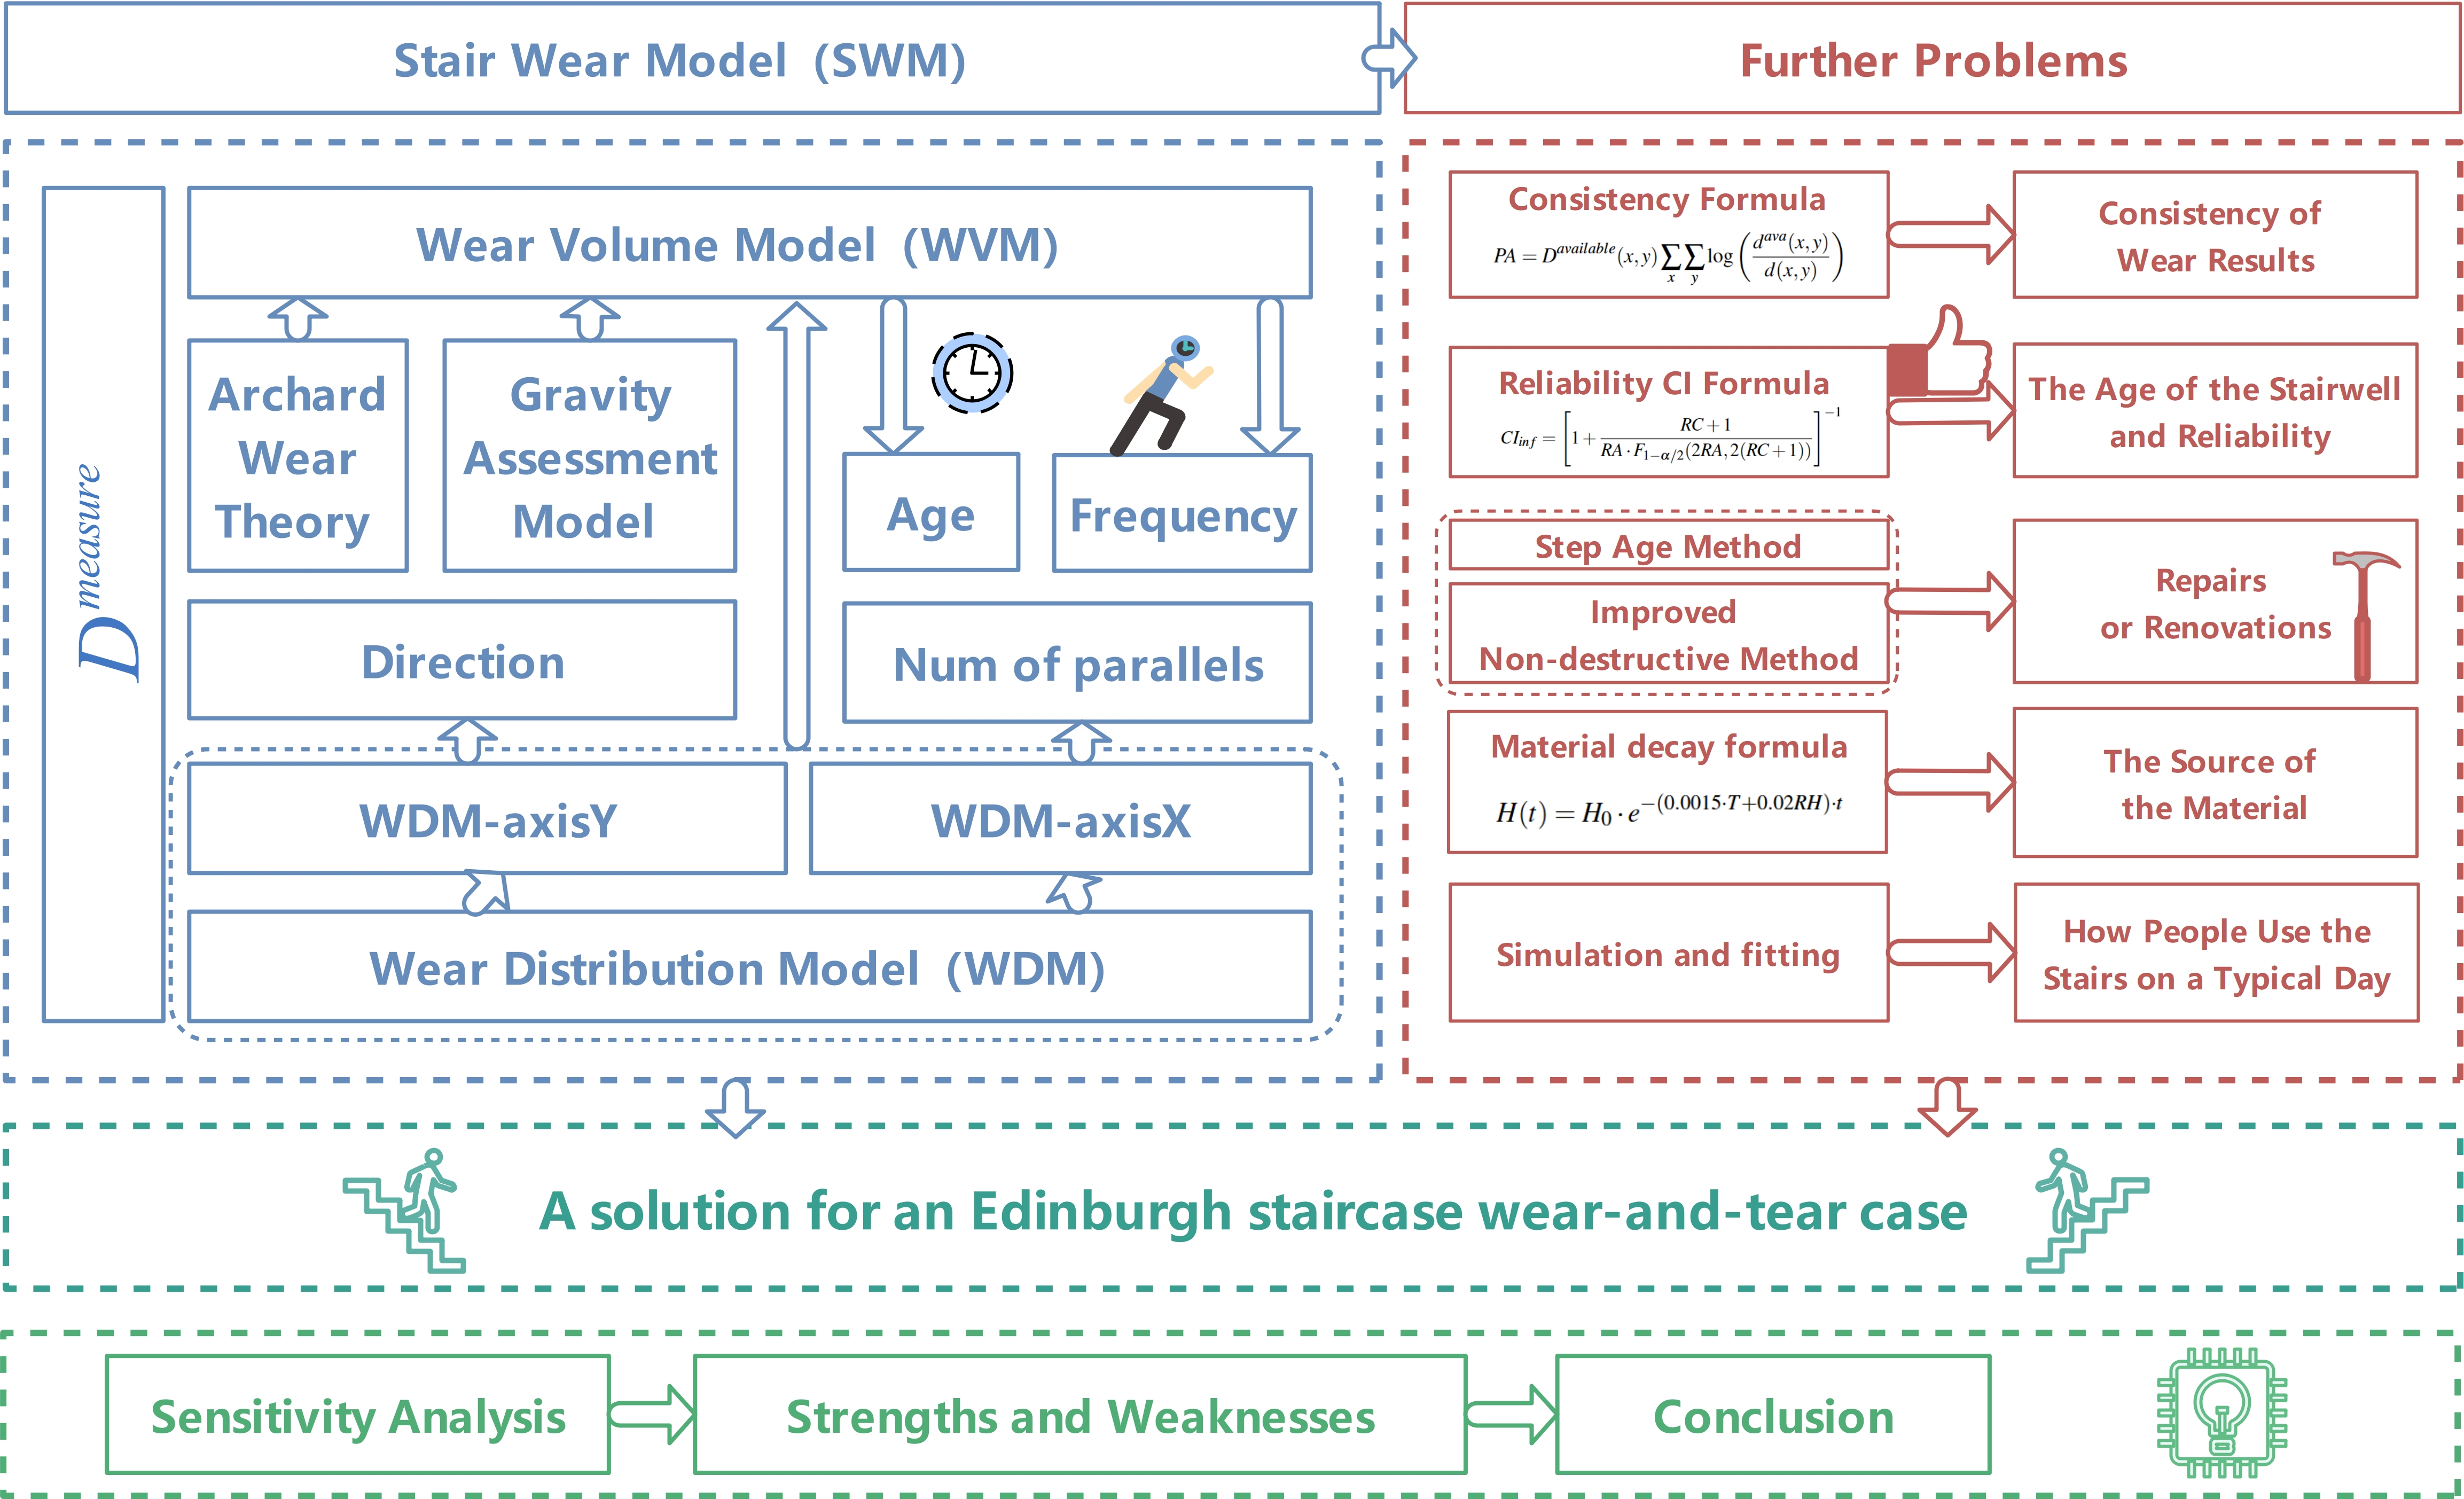
\includegraphics[width=1\linewidth]{美赛Latex模板/flowchat(Ourwork).jpg}
	\caption{The flowchart of our work}
	\label{ourwork_flowchart}
\end{figure}

% Chapter2 : 模型假设
\section{Assumptions and Notations}
%\vspace{-1.5em}
\subsection{Assumptions}
%\vspace{-1.0em}
To simplify the problem and make it convenient for us to simulate real-life conditions,we make the following basic assumptions, each of which is properly justified.
\begin{itemize}
	\setlength{\parsep}{0ex} %段落间距
	\setlength{\topsep}{2ex} %列表到上下文的垂直距离
	\setlength{\itemsep}{1ex} %条目间距
	\item \textbf{Assumption 1:}All people walk on the stairs with single-step strategy. the same set of steps in the same time subject to the same step.\\
    \textbf{Justification:} Single-step(SS) and double-step(DS) are two stepping strategies people prefer when walking on stairway steps\cite{1}. We choose the former strategy to ensure that all steps in a group are trampled equally.
    \vspace{1em}
    \item \textbf{Assumption 2:}
    Natural wear and other forms of erosion affect all surfaces of the same set of steps equally.
    \\
    \textbf{Justification:}
    The same set of steps is typically exposed to identical environmental conditions and is often constructed from the same materials. Since environmental factors are spatially uniform, it can be assumed that they exert the same effects on all surfaces of the steps.
    \vspace{1em}

    \item \textbf{Assumption 3:}
    Maintenance and renovation methods involve either completely replacing the stairs with another material or filling them with the same material to restore their original shape.
    \\
    \textbf{Justification:}
    These stairs primarily bear the wear load from people climbing upwards. It is essential to ensure that the repaired stairs possess sufficient wear resistance and load-bearing capacity to meet usage requirements. Therefore, replacing the entire material or meticulously filling with the same material ensures the structural integrity and durability of the stairs post-maintenance.
    \vspace{1em}

    \item \textbf{Assumption 4:}
    The force exerted by the shoe surface and the stair surface when climbing is uniformly directed downward.
    \\
    \textbf{Justification:}
    The shoe surface and the stair surface can be approximated as rigid bodies. In real environments, there are certainly frictional forces (for anti-slip or propulsion) and instantaneous mechanical changes caused by foot movements. However, for simplified analysis focusing solely on the overall load-bearing and wear amounts, smaller horizontal component forces or uneven distributions can be temporarily neglected. This results in an idealized "uniform vertical pressure model."

\end{itemize}

% Chapter3 : 符号说明
\vspace{-1.0em}
\subsection{Notations}
\begin{table}[H]
\vspace{-2.0em}
	\centering
        \caption{Notations Table}
        \renewcommand{\arraystretch}{1.5}
        \setlength{\tabcolsep}{16pt}
	\begin{tabular}{cc}
		\hline
		\hline
		\multicolumn{1}{c}{\textbf{Notations}} & \textbf{Definition}\\ \hline
        $d(x,y)$                       & The wear depth of the grid (x, y) on the step\\
        $D^{measure}$         & Wear measurement(x,y)
matrix\\
		$T$                      & The construction duration of the stair
\\
		$N_d$                      & Usage frequency of the step\\
		$G$                       & The average gravitational force experienced by walking people\\
        $k_m$                       & The amount of wear caused by unit force on the stone step\\
        $D(x,y)$                       & The foot traffic rate contributing to wear at point (x, y) on the stone step\\
        $k_m$                       & The wear coefficient of the material\\
        $d$                       & The sliding distance of contact on the tread surface of the step\\
        $H_0$                       & The initial material hardness\\
        $D_X$                       & The marginal function of $D(x,y)$ alone the $x$\\
        $D_Y$                       & The marginal function of $D(x,y)$ alone the $y$\\
        $RS(d_1, d_2)$                       & The correlation between two stone steps $d_1,d_2$\\
        $PA$                    &  The correlation between the two matrices\\
        $CI$                    &  The reliability of the age of the step\\
        
    \hline
		\hline
	\end{tabular}
\end{table}

\newpage
\section{Stair Wear Model}
Besides the wear information we are focusing on, for a step, the angle and the area of the steps are easy to get. The smaller the angle, the gentler the steps, making walking less strenuous. If the terrain in this area is relatively high, it might indicate that people have difficulty moving around. 

According to assumptions 1 and 2, people all use the single-step strategy (SS) to walk on the stairs. The rest of the factors have the same effect on the given set of steps. Therefore, in the absence of repairs, the condition of a single stone step gives a good picture of the age of a given set of steps, the traffic patterns of the people, and the daily patterns of life.  To acquire this interest information to archaeologists, we model the  Wear Volume Model and the Wear Distribution Model. Besides, we present the data that need to be measured. Finally, a set of ancient sandstone steps in Edinburgh is used as an example for solving the problems.
\subsection{Wear Volume Model}
\subsubsection{Rasterize The Surface of The Step}
In order to represent the actual physical steps by using a mathematical model for easy computer processing, we rasterize the steps. As shown in \autoref{Rasterization}, we take the top view of a step to obtain a rectangle with length $X$ m and width $Y$ m, which is discretized and divided into $m\times{n}$ rasters.

%\begin{figure}[H]
%	\centering
%	\includegraphics[width=0.9\linewidth]{美赛Latex模板/img/Rasterization.png}
%	\caption{Rasterized diagram of the stair surface}
%	\label{Rasterization}
%    \vspace{-2em} % 用来调间距
%\end{figure}

\begin{figure}[H]
	\centering
	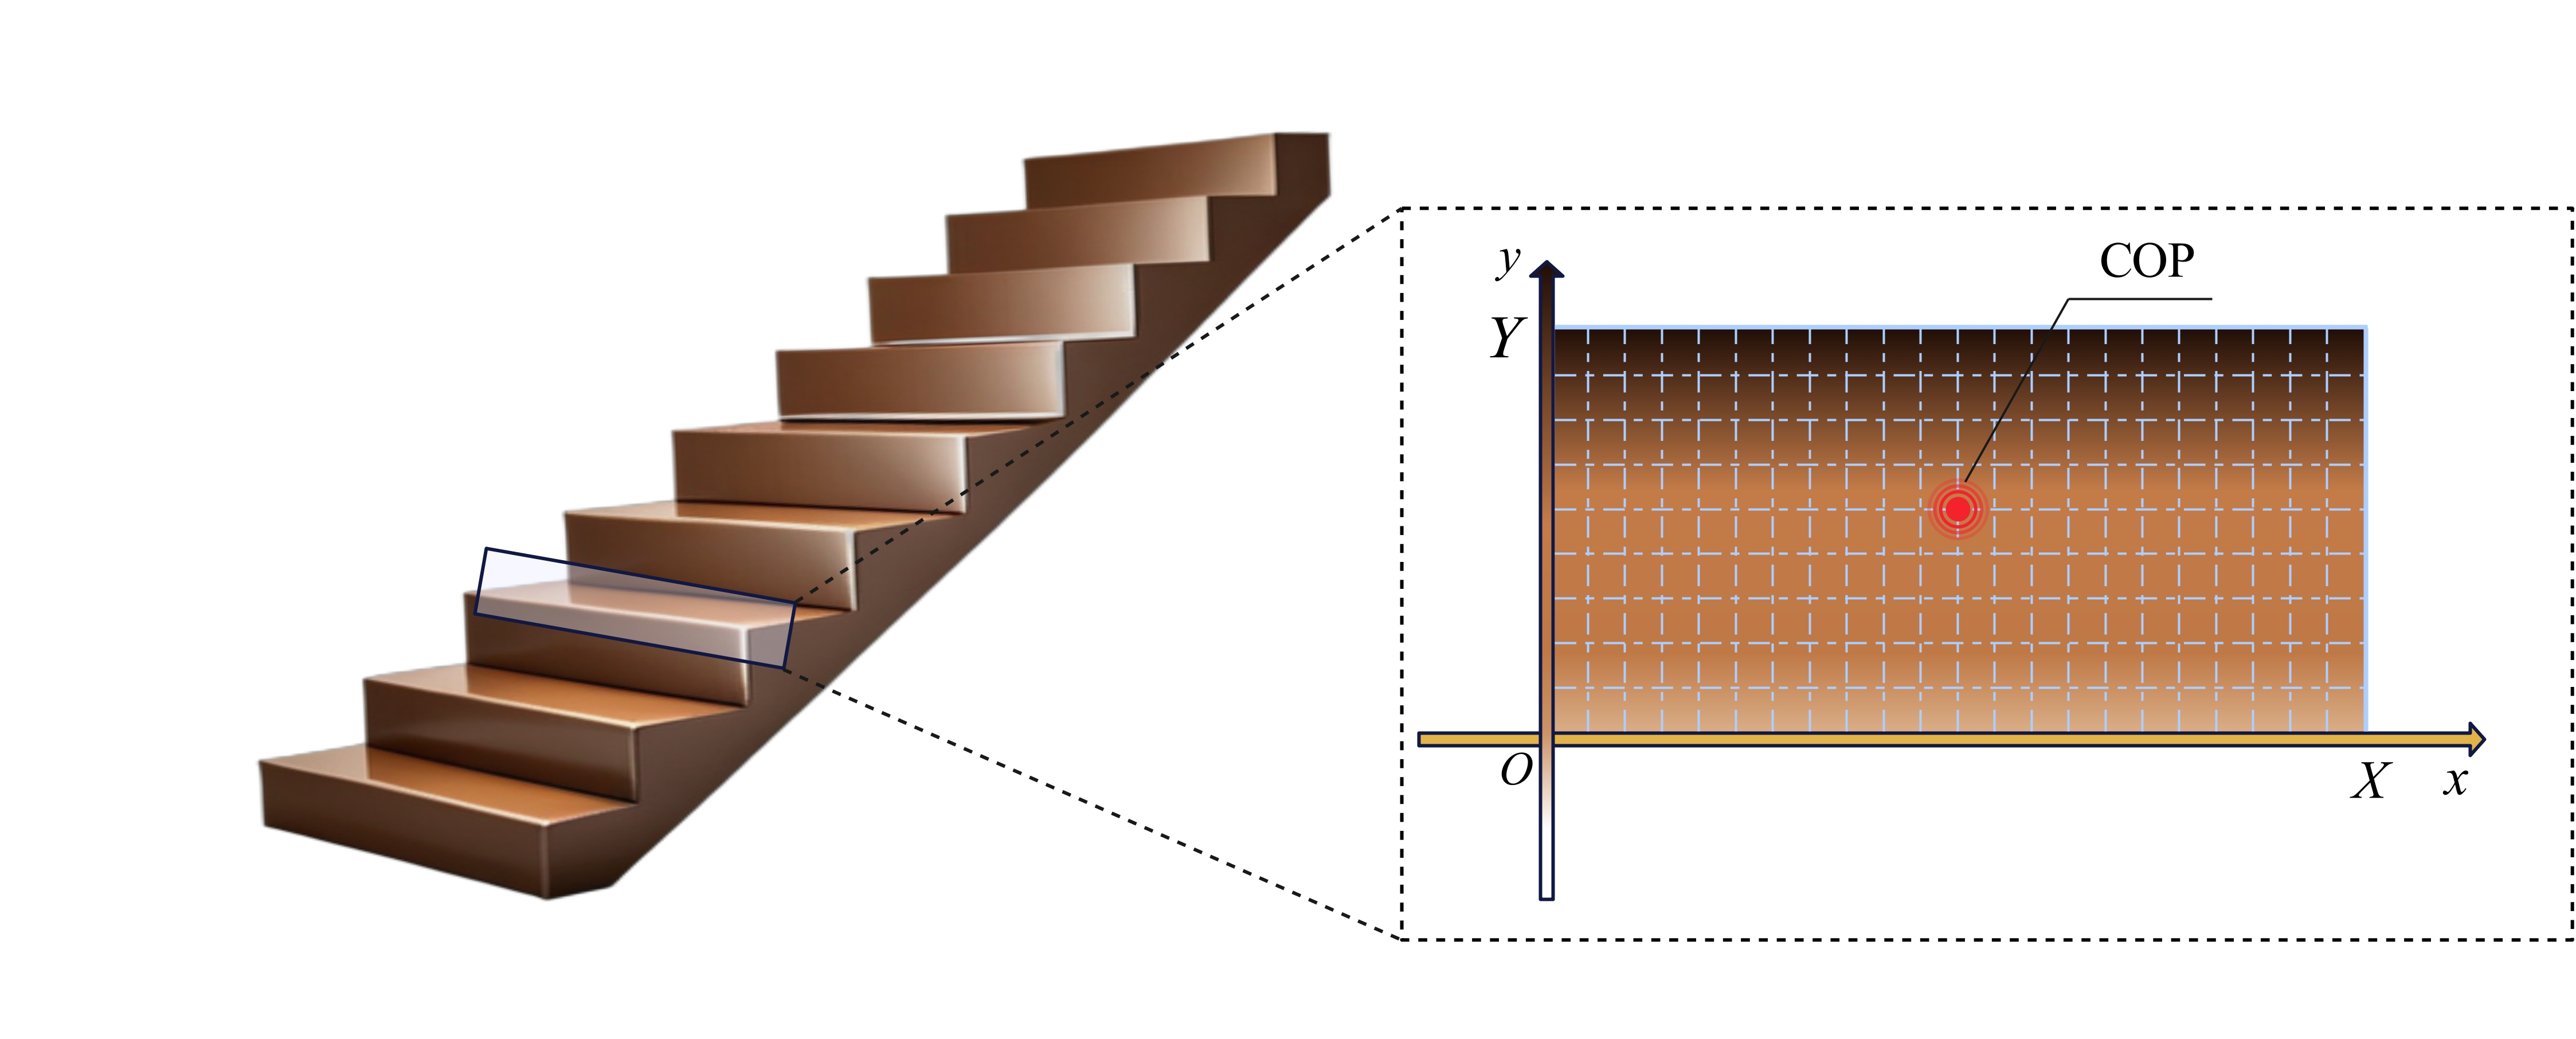
\includegraphics[width=0.9\linewidth]{美赛Latex模板/楼梯坐标1.jpg}
	\caption{Rasterized diagram of the stair surface}
	\label{Rasterization}
     \vspace{-2em} % 用来调间距
\end{figure}

The COP\cite{2} is defined as the center of each grid.
\begin{equation}
     x = \left\lfloor \frac{p}{G_s} \right\rfloor \quad,\quad y = \left\lfloor \frac{q}{G_s} \right\rfloor
\end{equation}
$p$ denotes the distance from this COP to the leftmost side of the step, $q$ denotes the distance from this COR to the bottom edge of the step, and $G_s$ is the size of the grid. $d(x,y)$ is defined as the amount of wear at grid COP(x,y). The archaeologist measures the wear volume of the stone steps and then constructs the measure wear matrix $D^{measure}(x,y)$.
\subsubsection{Wear Volumn Model}
Wear results from behavior over time for a material as hard as stone. The total number of steps taken on the same spot determines the amount of wear on that spot. The length of time determines the time scale of cumulative wear. The hardness and abrasion resistance of the material directly affects the wear rate. In addition, different distributions of steps and applied gravity in different areas can lead to uneven wear. In order to accurately obtain information about the steps, we introduced a comprehensive Wear Volume Model, combining the wear distribution model with the introduction of time, material, and number of footsteps:
\begin{equation}
    d(x,y) = T\cdot{N_d}\cdot{D(x,y)}\cdot{G}\cdot{k_m}
    \label{equation3.2}
\end{equation}

$d(x,y)$ represents the wear measured by the archaeologist, $T$ denotes the age of the stair, $N_d$ indicates the average number of people who walked the stairs each day, which is also known as usage frequency. $D(x,y)$ is the wear distribution function, we discuss it in Section 3.2. $G$ is the average gravitational force  experienced by walking people, and $k_m$ is defined as the wear volume coefficient (the amount of wear and tear per unit of $N$ on the stone steps). Further, we analyze the parameters $k_m$ and $G$.
\begin{itemize}
	\setlength{\parsep}{0ex} %段落间距
	\setlength{\topsep}{2ex} %列表到上下文的垂直距离
	\setlength{\itemsep}{1ex} %条目间距
	\item \textbf{Archard wear theory ($k_m$)} \\
\quad Archard wear theory is one of the classical wear models, proposed by J.F. Archard. The theory is used to describe the wear behavior of solid surfaces. Each step exerts a certain positive pressure on the step in the process, which can be directly applied to analyze the wear suffered by the step surface. At the same time, although the relative motion distance between the person and the step during walking is limited, the slight sliding of each step will cause localized wear on the step surface. Therefore, Archard's wear theory is applicable to analyze the wear of steps caused by people walking. The theory establishes the fundamental formula for the unit wear coefficient of a solid $k_m$, which is defined as:
\begin{equation}
    k_m = K\cdot{\frac{d}{H}}
\end{equation}
where $K$ denotes the stone wear coefficient, $d$ represents the relative sliding distance of the tread surface, and $H$ indicates the material hardness of the stone. 

\quad Material hardness $H$ is not static but varies with time, resulting from physical factors (such as temperature changes and wind erosion) and chemical weathering (such as hydrolysis and oxidation). Hence, we use an \textbf{exponential decay model }to simulate the loss of hardness caused by weathering of rocks:
\begin{equation}
    H(t)=H_0⋅e^{{-}{pt}}
\end{equation}
$H_0$ denotes the initial material hardness while $p$ denotes the weathering rate constant. Moreover, another form of relationship between hardness and age can be provided:
\begin{equation}
    {H}{T}=\int_{t}H(t)
    \label{eq:HT} 
\end{equation}

Based on the site survey, an information review is needed to obtain $K$, $H_0$ and $p$.

   \item \textbf{Gravity Assessment Model ($G$)}\\
   \quad The same step may be used by people of different ages and genders with different weight characteristics. We categorize the population into six groups: male minors (mm), female minors (fm), adult males (am), adult females (af), older men (om), older women (ow). To make the results more precise, we use their weight expectation as $W$ in the model, which is calculated as follows:
    \begin{equation}
        W=\sum_{i}u_i\cdot{q_i}
    \end{equation}
    \end{itemize}
    \quad where $u_i$ describes the average weight of each population, $q_i$ indicates the proportion of each population to the total population. 
    
    \quad If they do not have this information, based on the global weight data provided by the World Health Organization (WHO)\cite{6}\cite{7}, we provide the reference data as shown in \autoref{weight_data}.

    \begin{table}[H]
    \centering
    \caption{Global Average Weight and Population Proportion by Age and Gender Group}
    \renewcommand{\arraystretch}{1.5}
    \setlength{\tabcolsep}{12pt}
    \begin{tabular}{ccc}
        \hline
        \hline
        \textbf{Population Group} & \textbf{Average Weight ($kg$)} & \textbf{Proportion ($\%$)} \\
        \hline
        Male Minors (mm) & 40 & 10 \\
        Female Minors (fm) & 38 & 10 \\
        Adult Males (am) & 75 & 30 \\
        Adult Females (af) & 65 & 30 \\
        Older Men (om) & 70 & 10 \\
        Older Women (ow) & 60 & 10 \\
        \hline
        \hline
    \end{tabular}
    \label{weight_data}
\end{table}


\quad The overall average weight of the population is $W = 62.8\,\mathrm{kg}$. This average is typically calculated as a weighted sum of the proportions $q_i$ and the average weights $u_i$ of each subgroup. To obtain a more precise estimate, archaeologists or researchers can adjust the subgroup proportions $q_i$ or their average weights $u_i$ to better reflect more localized or up-to-date demographic data.This can make the calculation results more accurate and increase the flexibility of the model.

\quad This adjustment allows for a more accurate estimation of the gravitational force $G$. The gravitational force is calculated using the following formula:
\begin{equation}
    G = W \cdot g
\end{equation}
where $g = 9.81\,\mathrm{m/s^2}$ \cite{9}is the acceleration due to gravity.


Integrating \autoref{equation3.2}, we obtain the expression for the average wear $d_{avg}$ as
\begin{equation}
    d_{avg} = \frac{1}{A_{ceff}}\int_{A_{ceff}} T\cdot{N_d}\cdot{D(x,y)}\cdot{G}\cdot{k_m}dxdy
\end{equation}
in this equation, $A_{ceff}$ denotes the area of the steps overlook.

\subsubsection{Calculation of Age and Frequency of Stone Steps}
According to the analysis above, When $D$,$G$, and $k_m$ are determined,  the age of stone step $T$ and frequency of use $N_d$ can be solved for each other. The specific formulas are shown below:
\begin{equation}
    T = \frac{A_{ceff}\cdot{d_{avg}}}{N_d\cdot{G}\cdot{k_m}}
\end{equation}
\begin{equation}
    N_d = \frac{A_{ceff}\cdot{d_{avg}}}{T\cdot{G}\cdot{k_m}}
\end{equation}
At this point, the age of the stone step $T$ and frequency of use $N_d$ can be sought.

\subsection{Wear Distribution Model}
Each step on the steps can be regarded as obeying independently and identically distributed. Research shows a linear relationship between the number of steps and the amount of wear, and only when the cumulative number of steps reaches a large size, significant wear on the surface of the step stone can be produced.  According to the \textbf{Central Limit Theorem}, when the number of independent random samples is large enough, even if the original distribution is not normal, the distribution of the sample mean and sum will converge to the normal distribution. Therefore, when the sample size is large, the cumulative distribution of steps tends to be normal, and the cumulative wear will also be normal.

Since there is no significant correlation between the lateral and longitudinal positions of the footsteps on the stone stairs, the cumulative wear of pedestrians at each position in both the x- and y-directions can be described as a superposition of normal or multi-normal distributions when the number of steps is sufficiently high. And the distributions reflect the traffic patterns of people on that set of stairs.
\subsubsection{Wear Distribution in The Y-direction - Judging The Direction}
Studies of the gait cycle show that during stair ascent, the first peak appears in the heel, while during stair descent, the first peak is in the forefoot. This is shown in \autoref{fig:ForceDiagram}. In addition, observing people's daily stair movement behavior, it is found that pedestrians' point of impact is closer to the lower edge of the steps when going up the stairs than when going down the stairs\cite{3}. 
\begin{figure}[H]
\vspace{-1.0em}
	\centering    
	\subfigure[stair ascent]{				% 图片1([]内为子图标题)
		\label{fig:showup}							% 子图1的标签
		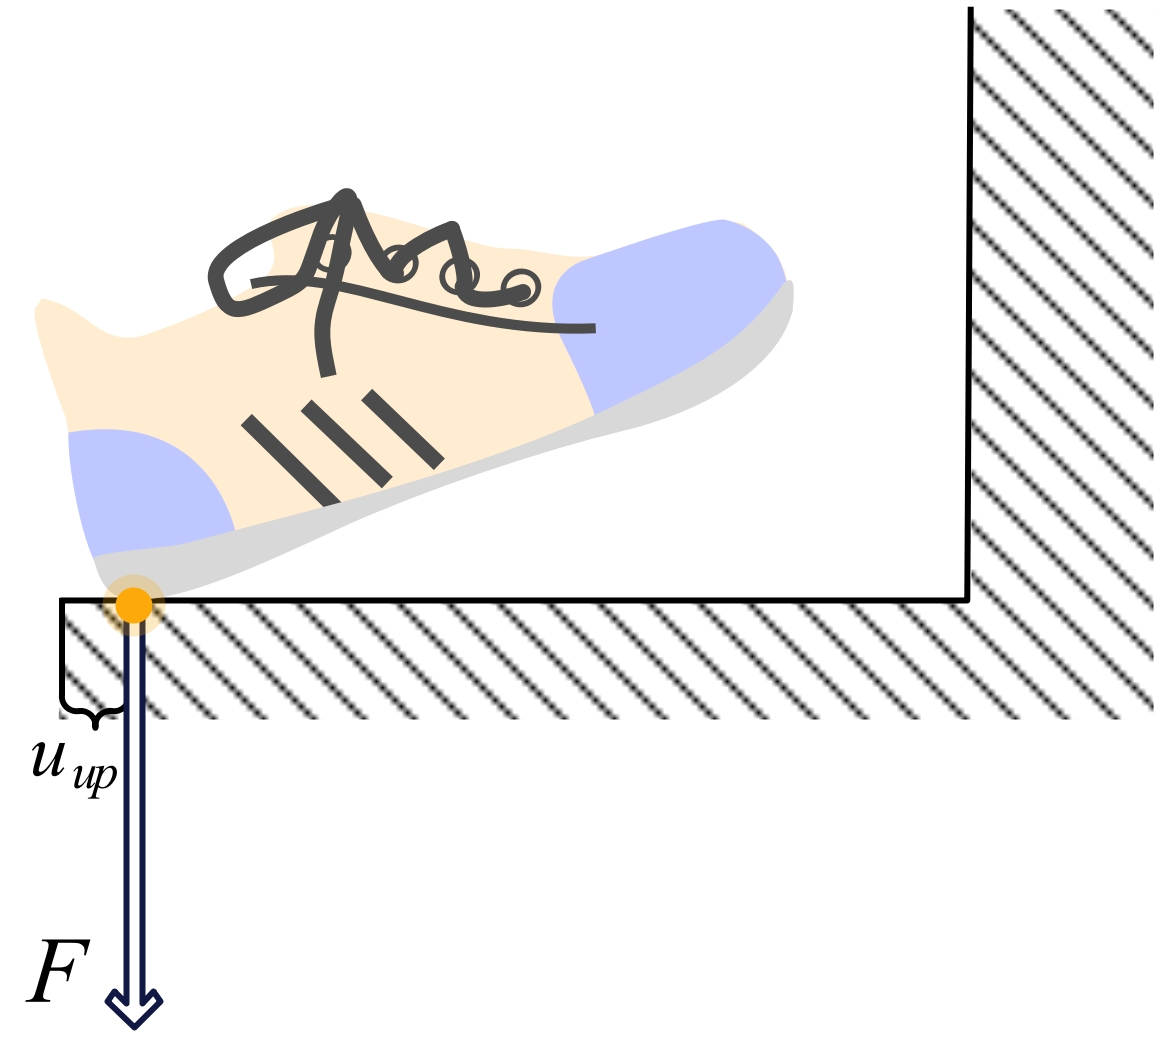
\includegraphics[width=0.4\textwidth]{美赛Latex模板/shoeUp.jpg}}% 子图1的相对位置
	\subfigure[stair descent]{				% 图片2
		\label{fig:showDown}						% 子图2的标签
		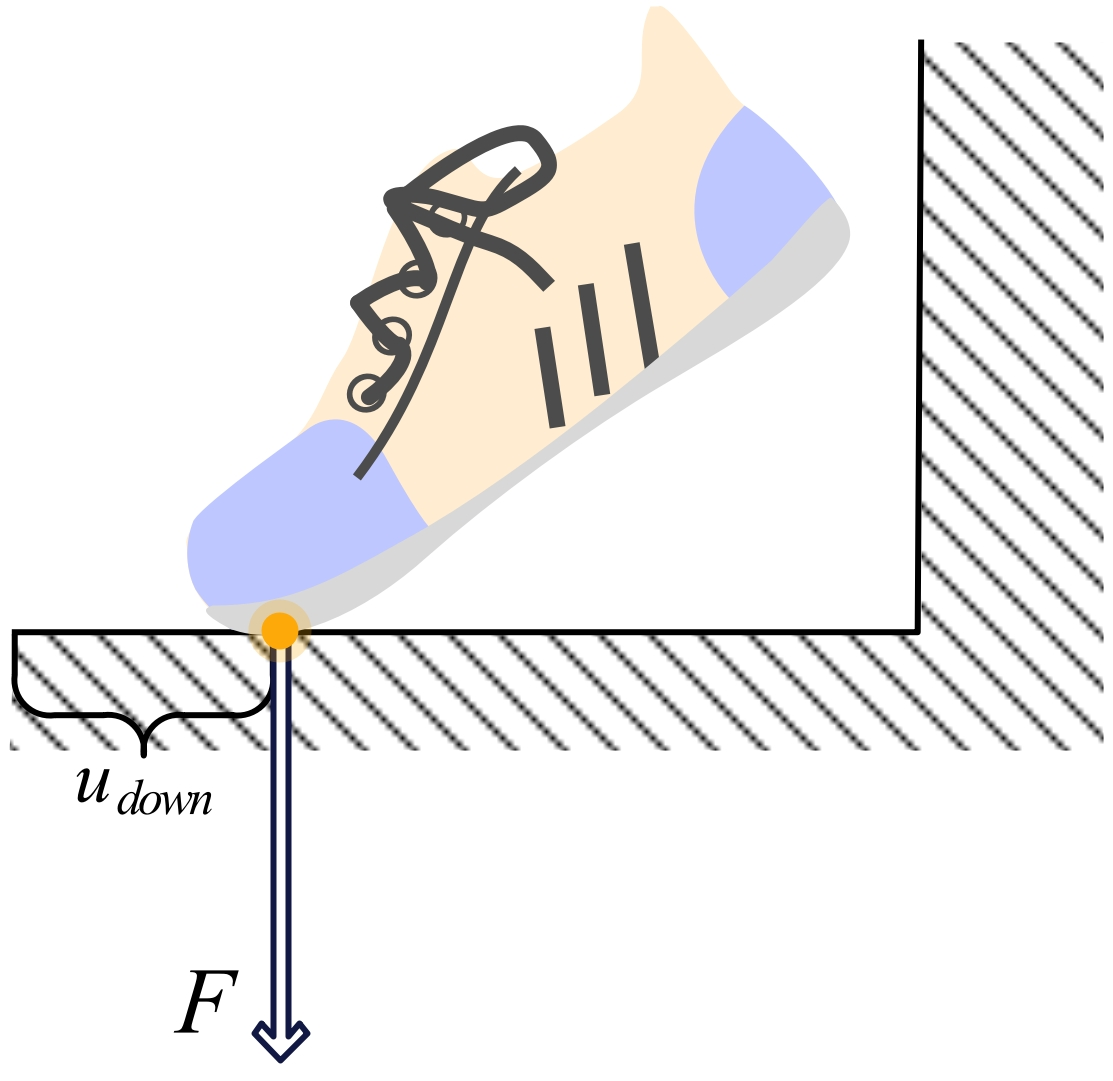
\includegraphics[width=0.4\textwidth]{美赛Latex模板/shoeDown.jpg}}% 子图2的相对位置
	\caption{Force diagram of walking}		% 总图标题
	\label{fig:ForceDiagram}									% 总图标签
    \vspace{-1.0em}
\end{figure}

With the conclusion above, we can judge whether people using the stairs favored a certain direction of travel based on the wear distribution of Y-direction. 

\begin{figure}[H]
\vspace{-1.0em}
	\centering    
	\subfigure[Double direction - Wear Distribution]{				% 图片1([]内为子图标题)
		\label{fig:doua}							% 子图1的标签
		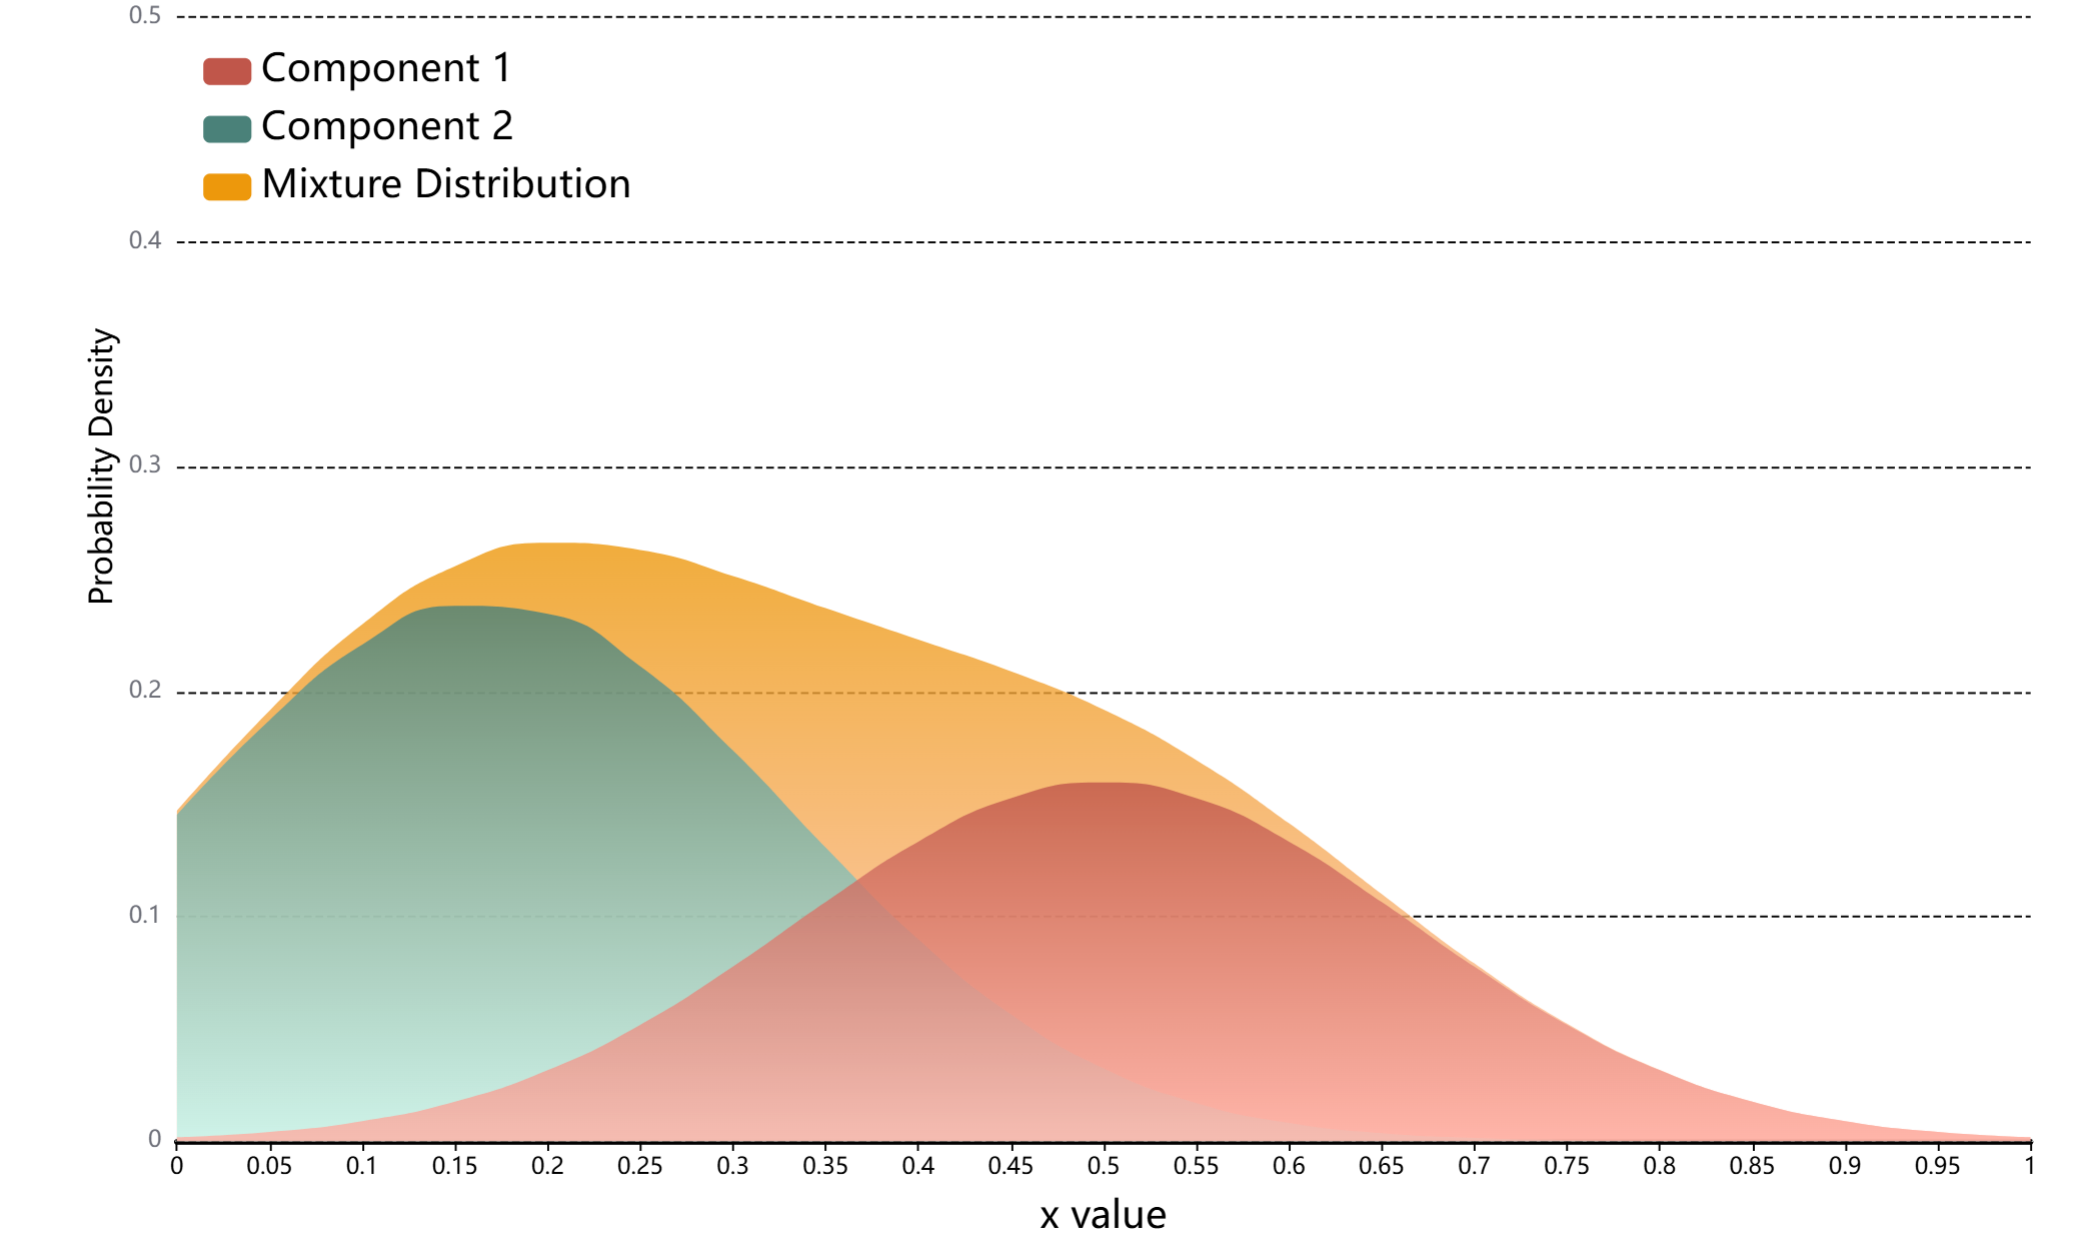
\includegraphics[width=0.45\textwidth]{美赛Latex模板/965377162c7977beb14a645b57f5f304.png}}% 子图1的相对位置
	\subfigure[Double direction]{				% 图片2
		\label{fig:doub}						% 子图2的标签
		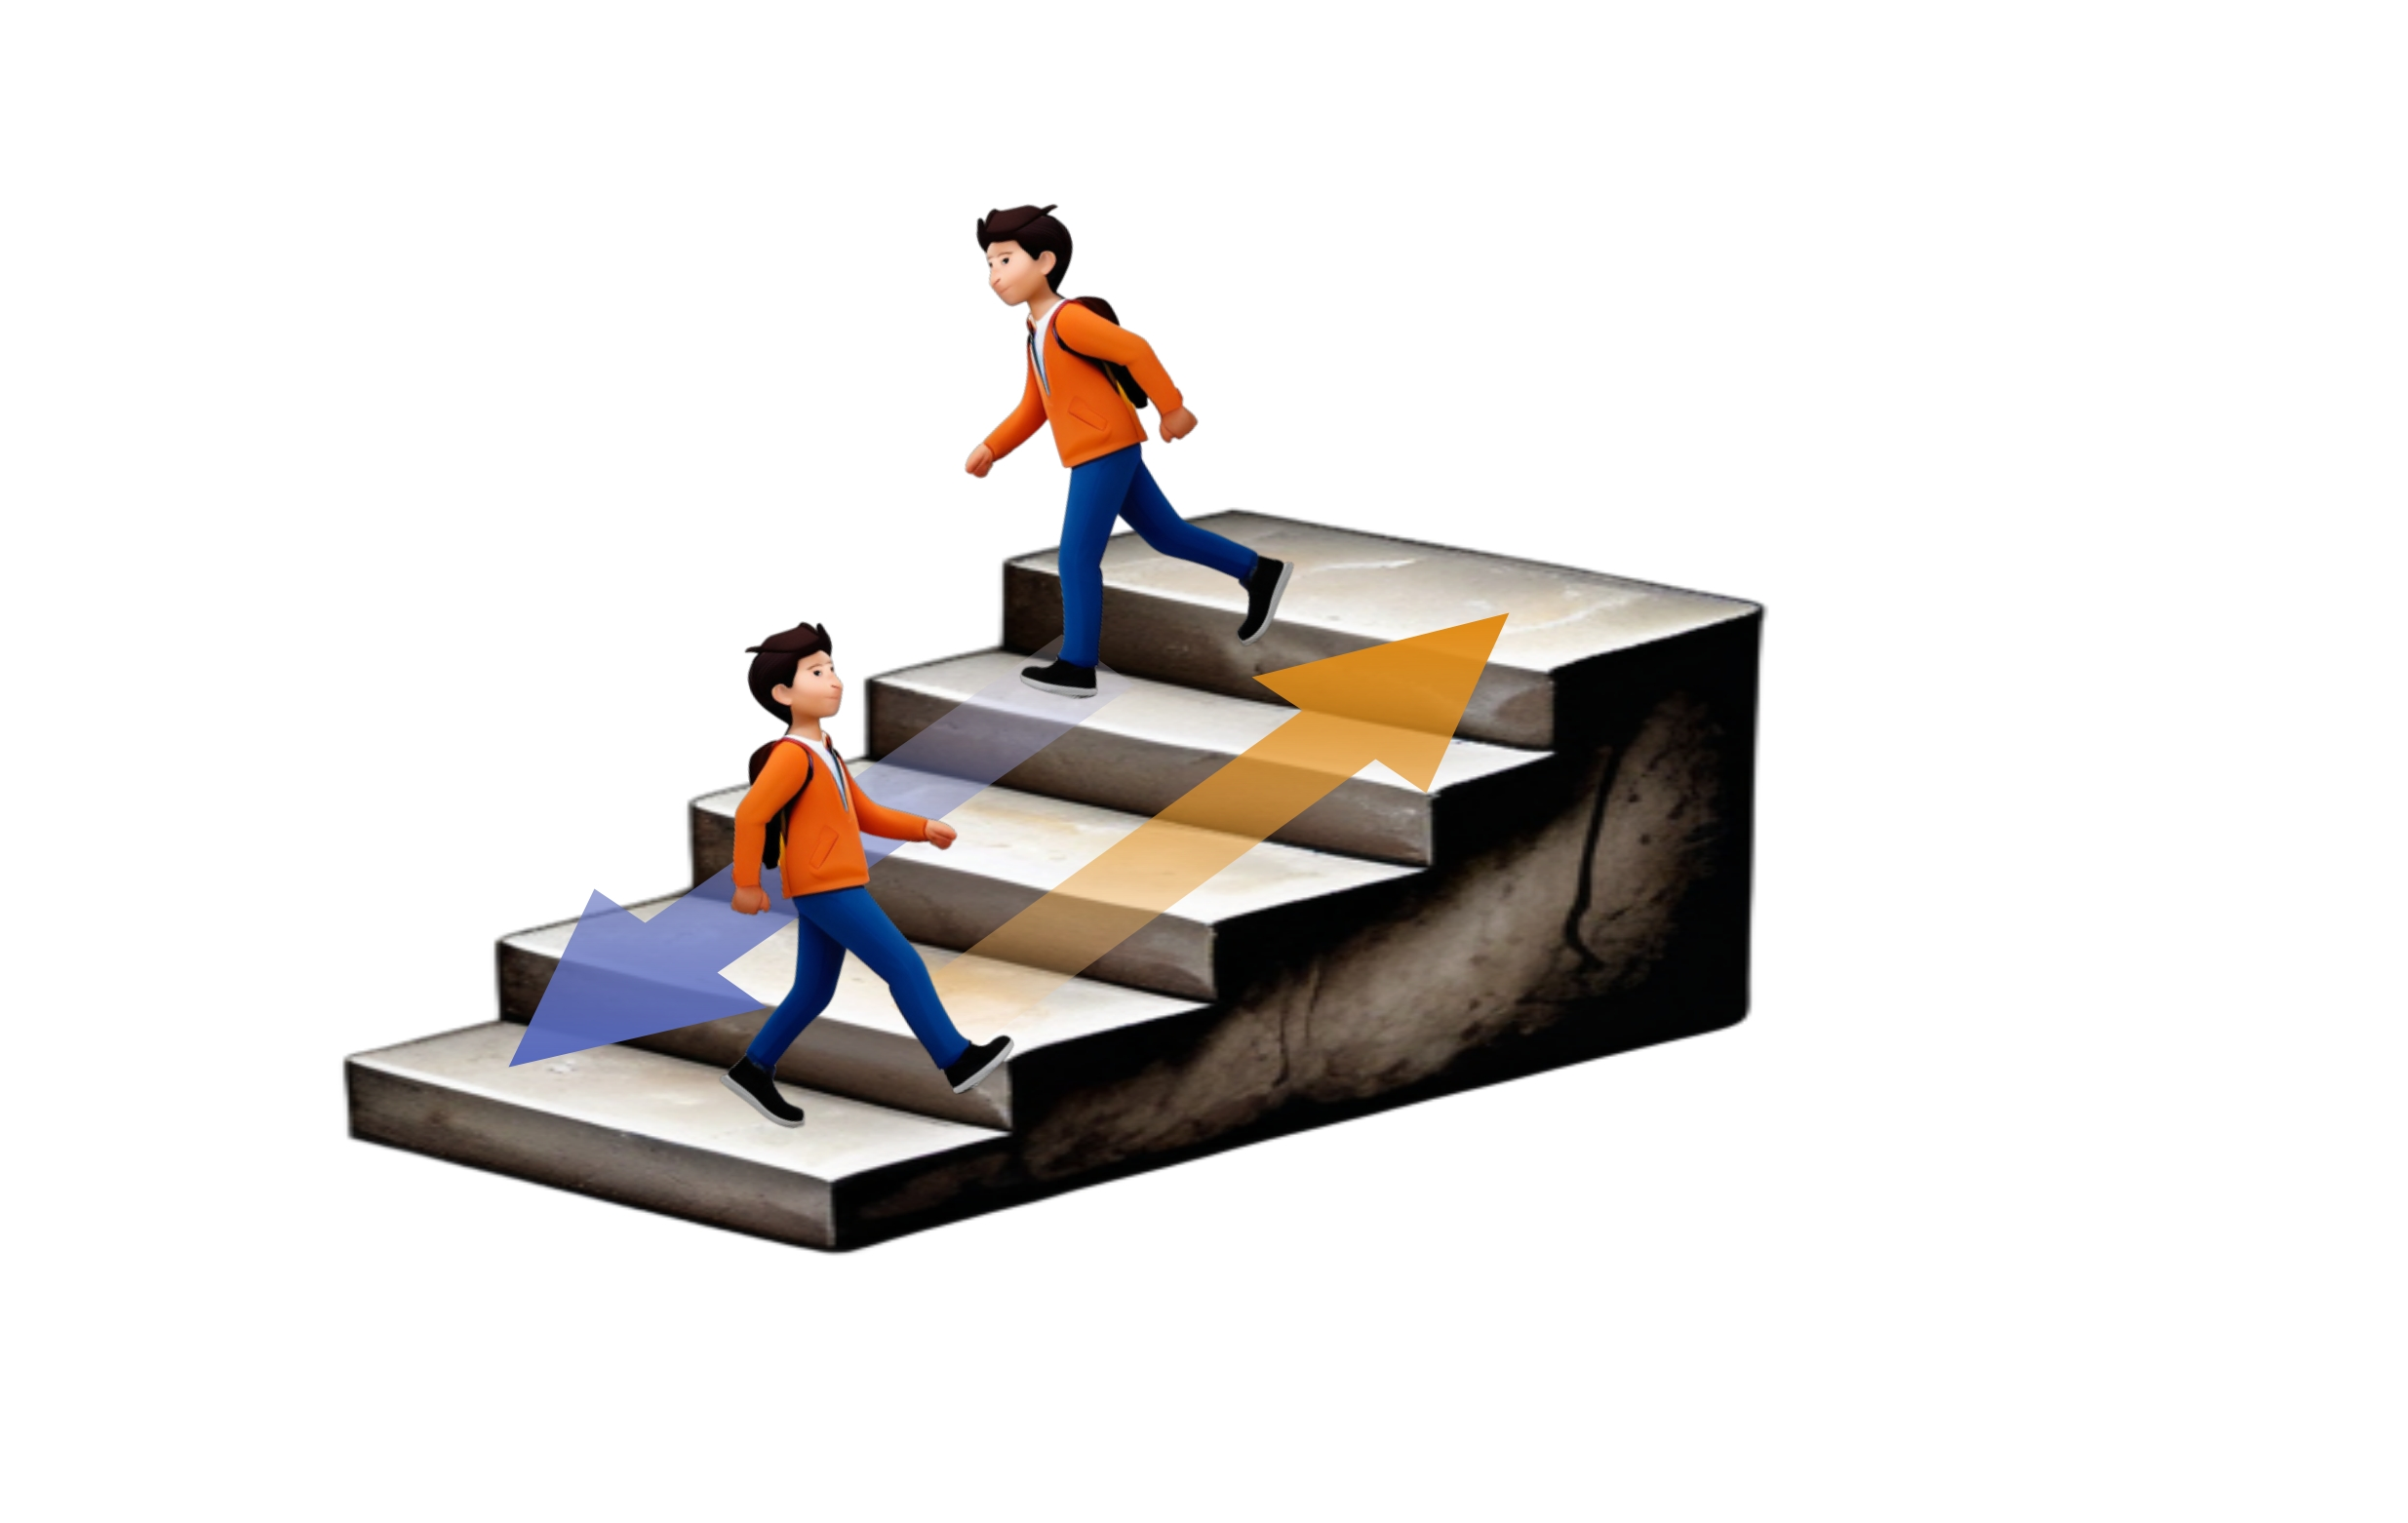
\includegraphics[width=0.45\textwidth]{美赛Latex模板/双向通行.jpg}}% 子图2的相对位置
    \vspace{-1.0em}
    \\
    \subfigure[Upward Direction - Wear Distribution]{				% 图片3([]内为子图标题)
		\label{fig:upa}							% 子图3的标签
		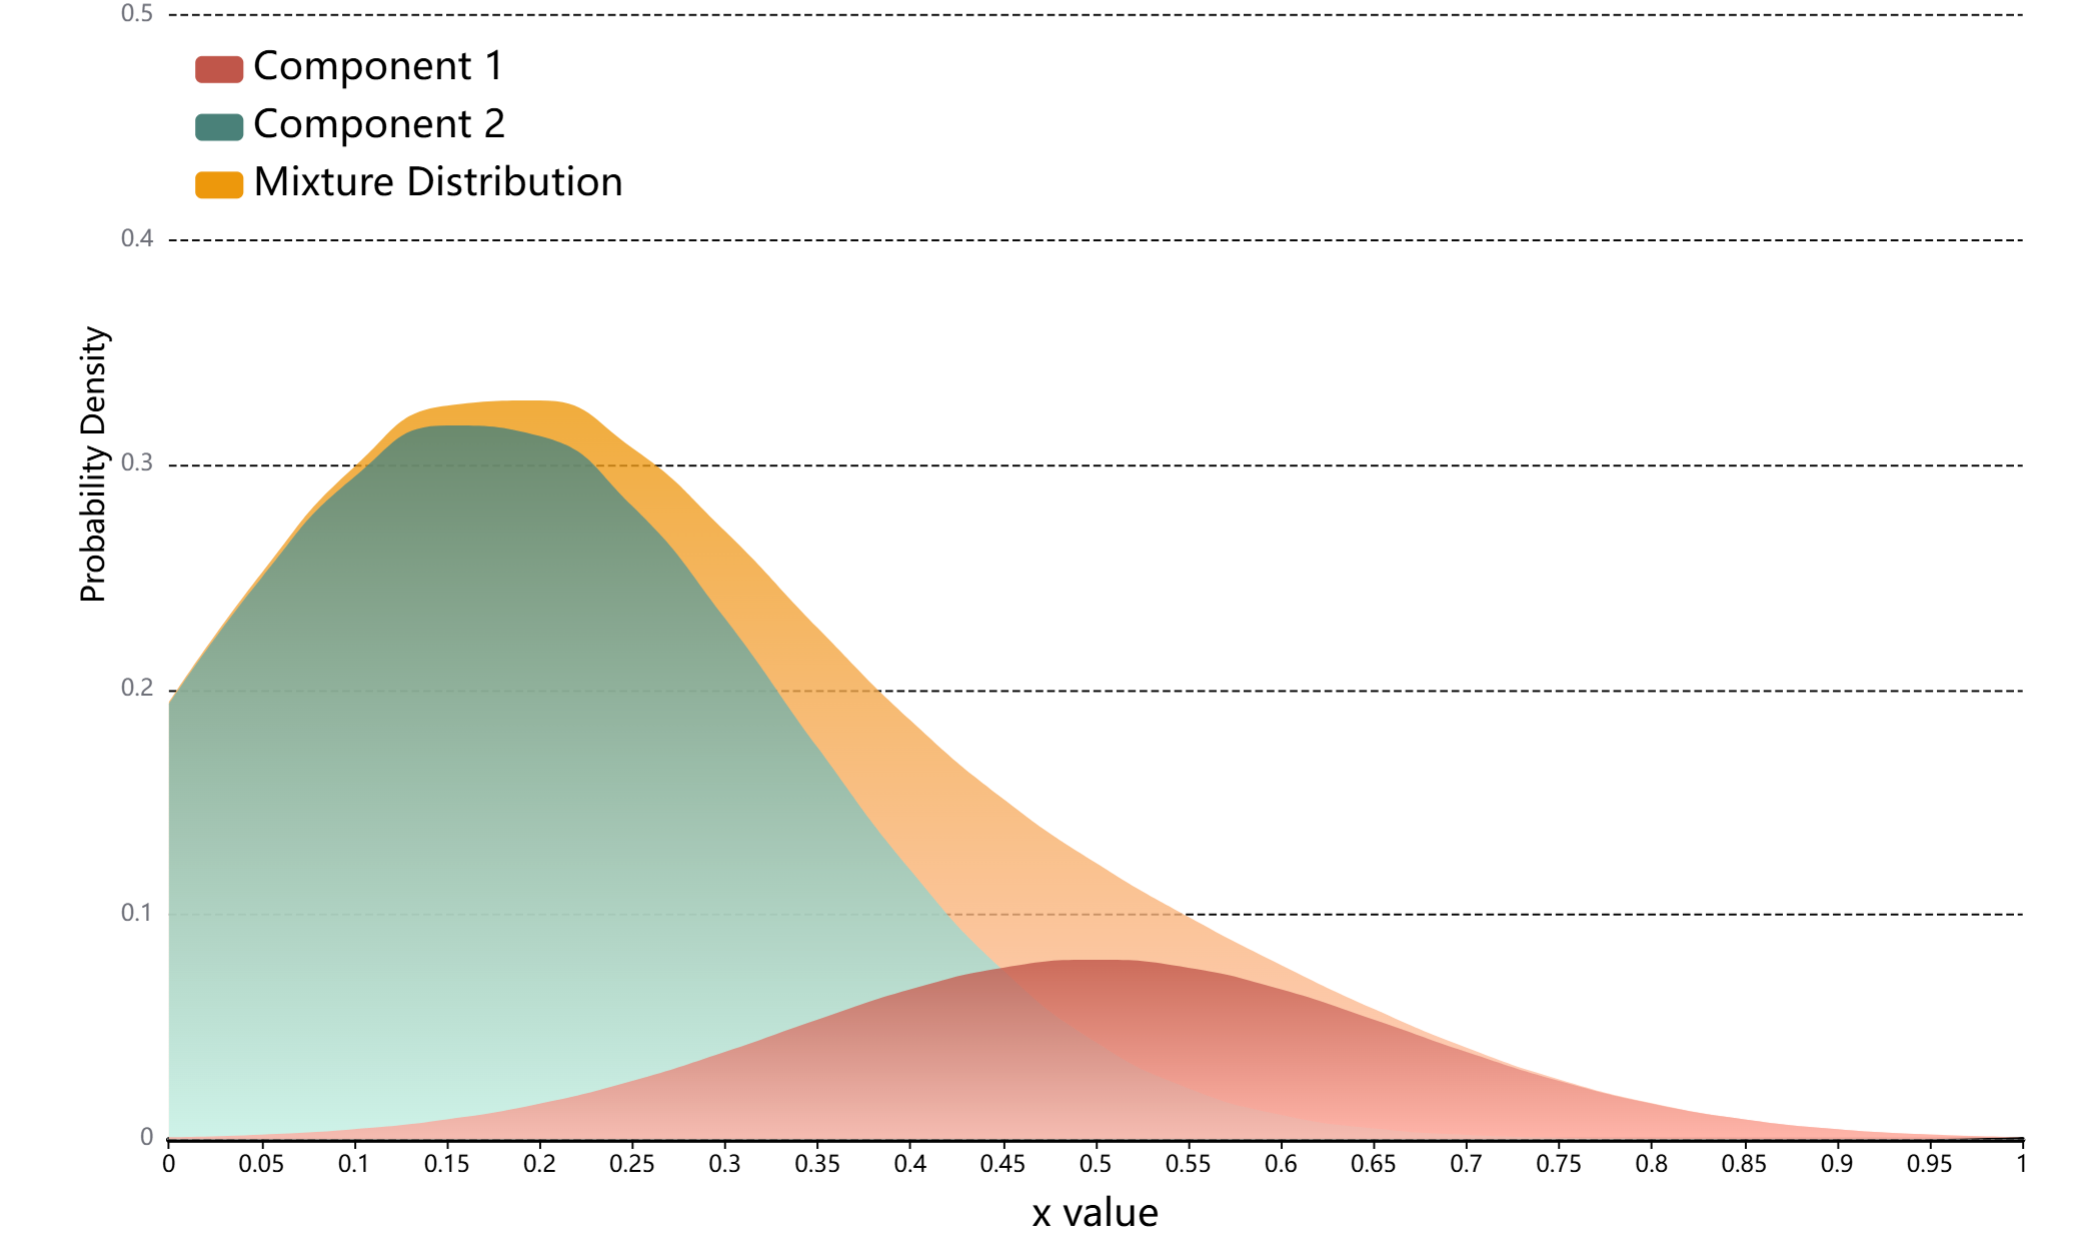
\includegraphics[width=0.45\textwidth]{美赛Latex模板/cd9eecd1e0650a654c291cc6dca93f35.png}}% 子图3的相对位置
	\subfigure[Upward Direction]{				% 图片4
		\label{fig:ipb}						% 子图4的标签
		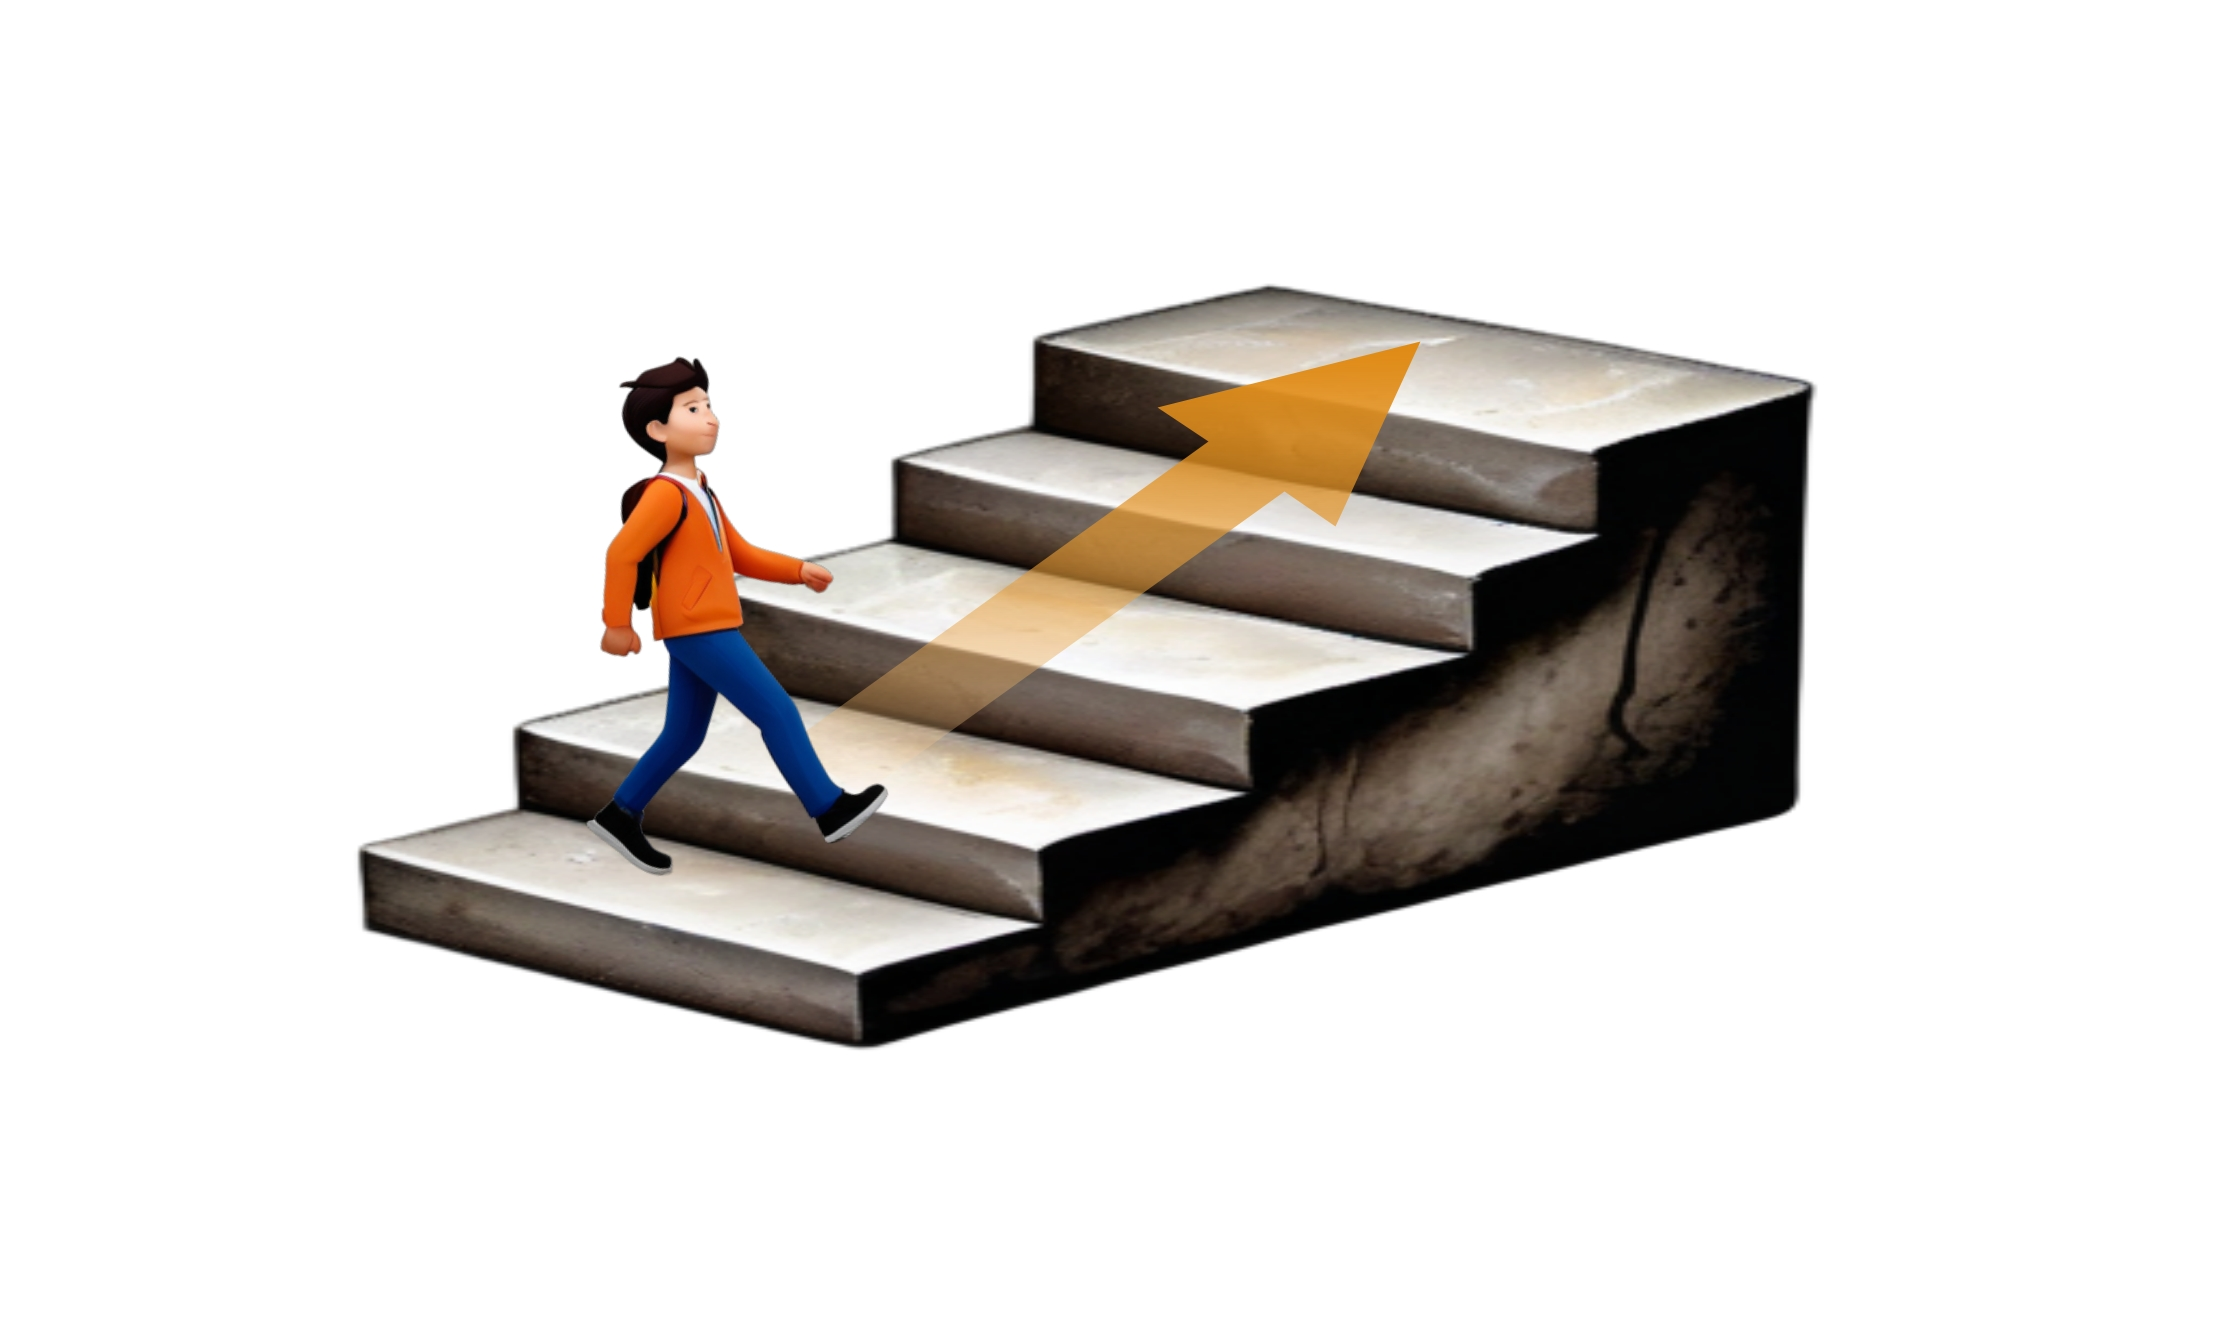
\includegraphics[width=0.45\textwidth]{美赛Latex模板/单行.jpg}}% 子图4的相对位置
	\caption{Distribution of wear in the Y-direction and the corresponding people}		% 总图标题
	\label{fig:Y-two}									% 总图标签
    \vspace{-1.0em}
\end{figure}

As shown in \autoref{fig:Y-two}(a),  there are two peaks, which means that the marginal distribution in the y-direction is a superposition of two normal distributions. This indicates that stairs were usually used in both directions. The number of people traveling up and down the stairs can be compared based on the size of the peaks. Similarly, one peak in \autoref{fig:Y-two}(c) demonstrates that people using the stairs favored a certain direction of travel. If the y-value at the peak is small, people favored upward travel. If it is larger, downward travel was favored.


We further quantify the results so that archaeologists can determine the direction and the proportion of up-and-down people more intuitively. Using knowledge of probability statistics, we construct the distribution of wear in the Y-direction:
\begin{equation}
D_{y}\sim w_{up}\cdot N_i(\mu_{up},\sigma_{up})+w_{down}\cdot N_i(\mu_{down},\sigma_{down})
\end{equation}
$w_{up}$ denotes the ratio of people going up to the total number of people, while $w_{down}$ denotes the ratio of people going down to the total number of people. $\mu_{up}$ is the distance between the center of the stepping surface of the person going up and the outermost part of the stone step, and $\mu_{down}$ is the distance between the center of the stepping surface of the person going down and the outermost part of the stone step. $\sigma_{up}$ describes the degree of longitudinal dispersion of people going upstairs, and $\sigma_{down}$ describes the degree of vertical dispersion downstairs. 
\subsubsection{Wear Distribution in The X-direction - Calculating The Number of Parallels}
When people walk on the stairs in a single-step strategy, the peaks of the normal distribution in the X-direction of the steps describe the main concentration area of pedestrians. And the number of peaks reflects the lateral distribution characteristics of pedestrians on the road. We describe the wear distribution in this direction as:
\begin{equation}
    D_{x}\sim w_i\sum_{i}N_i(\sigma_i,\mu_i)
\end{equation}
$n$ represents the number of parallel lanes on the same step of the stone staircase, $w_i$ is the ratio of the number of people in the lane $i$ to the total number of people,  $\mu_i$ denotes the distance of the center of the lane $i$ from the leftmost end of the stone staircase, and $\sigma_i$ indicates the degree of lateral dispersion of lane $i$.

\begin{figure}[H]
\vspace{-1.0em}
	\centering    
	\subfigure[Travel single - Wear distribution]{				% 图片1([]内为子图标题)
		\label{fig:singlea}							% 子图1的标签
		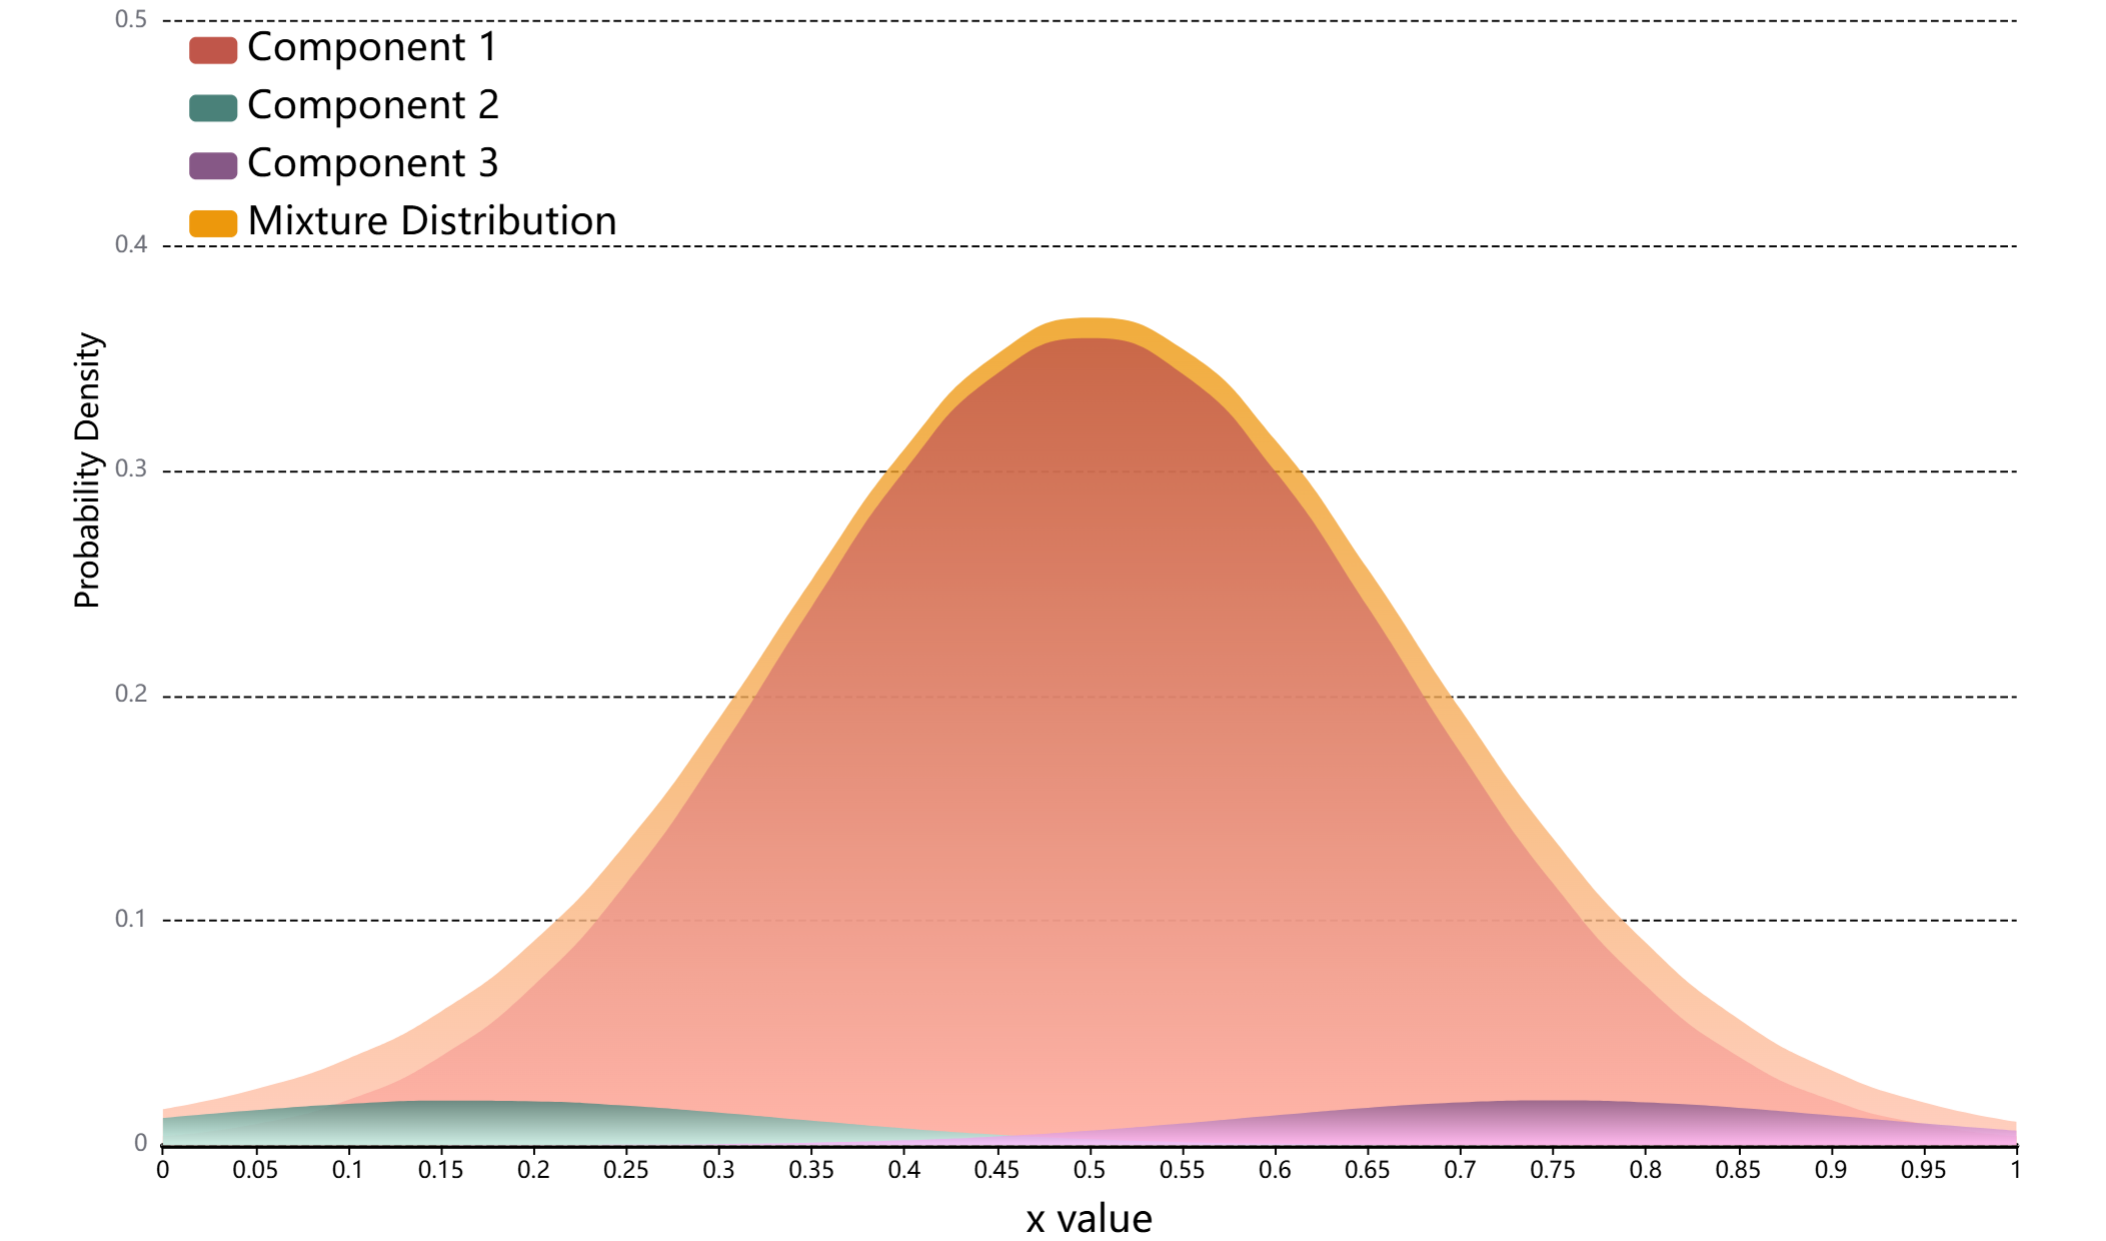
\includegraphics[width=0.4\textwidth]{美赛Latex模板/2cbb0fefdd82765982db1289686f9d28.png}}% 子图1的相对位置
	\subfigure[Travel single]{				% 图片2
		\label{fig:singleb}						% 子图2的标签
		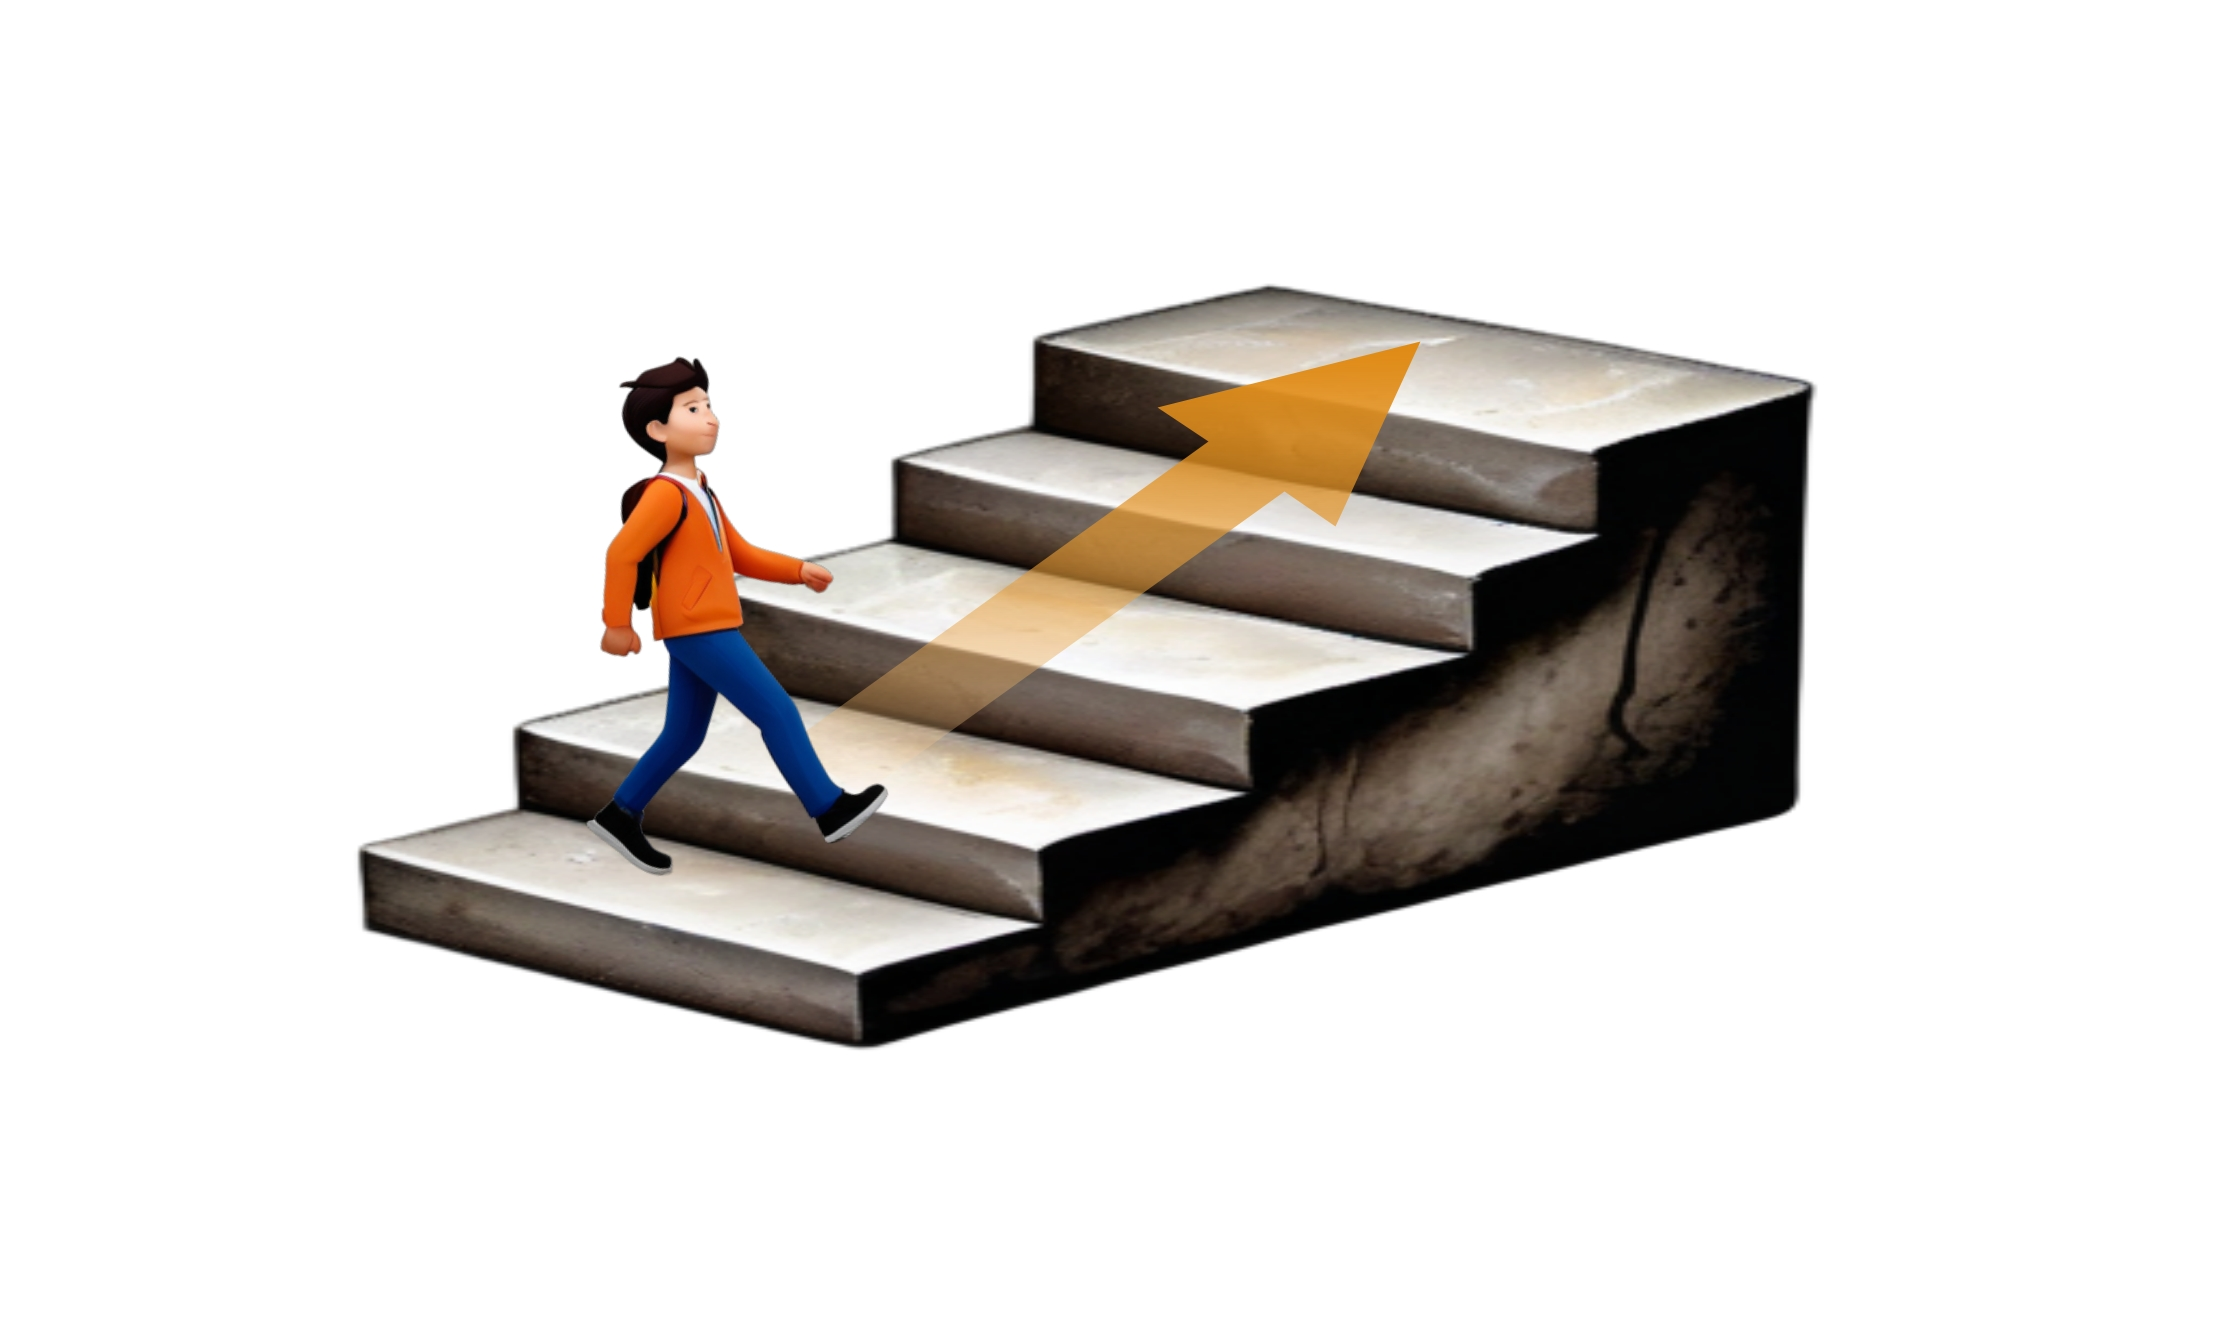
\includegraphics[width=0.4\textwidth]{美赛Latex模板/单行.jpg}}% 子图2的相对位置
    \vspace{-1.0em}
    \\
    \subfigure[Side by side - Wear distribution]{				% 图片3([]内为子图标题)
		\label{fig:twoa}							% 子图3的标签
		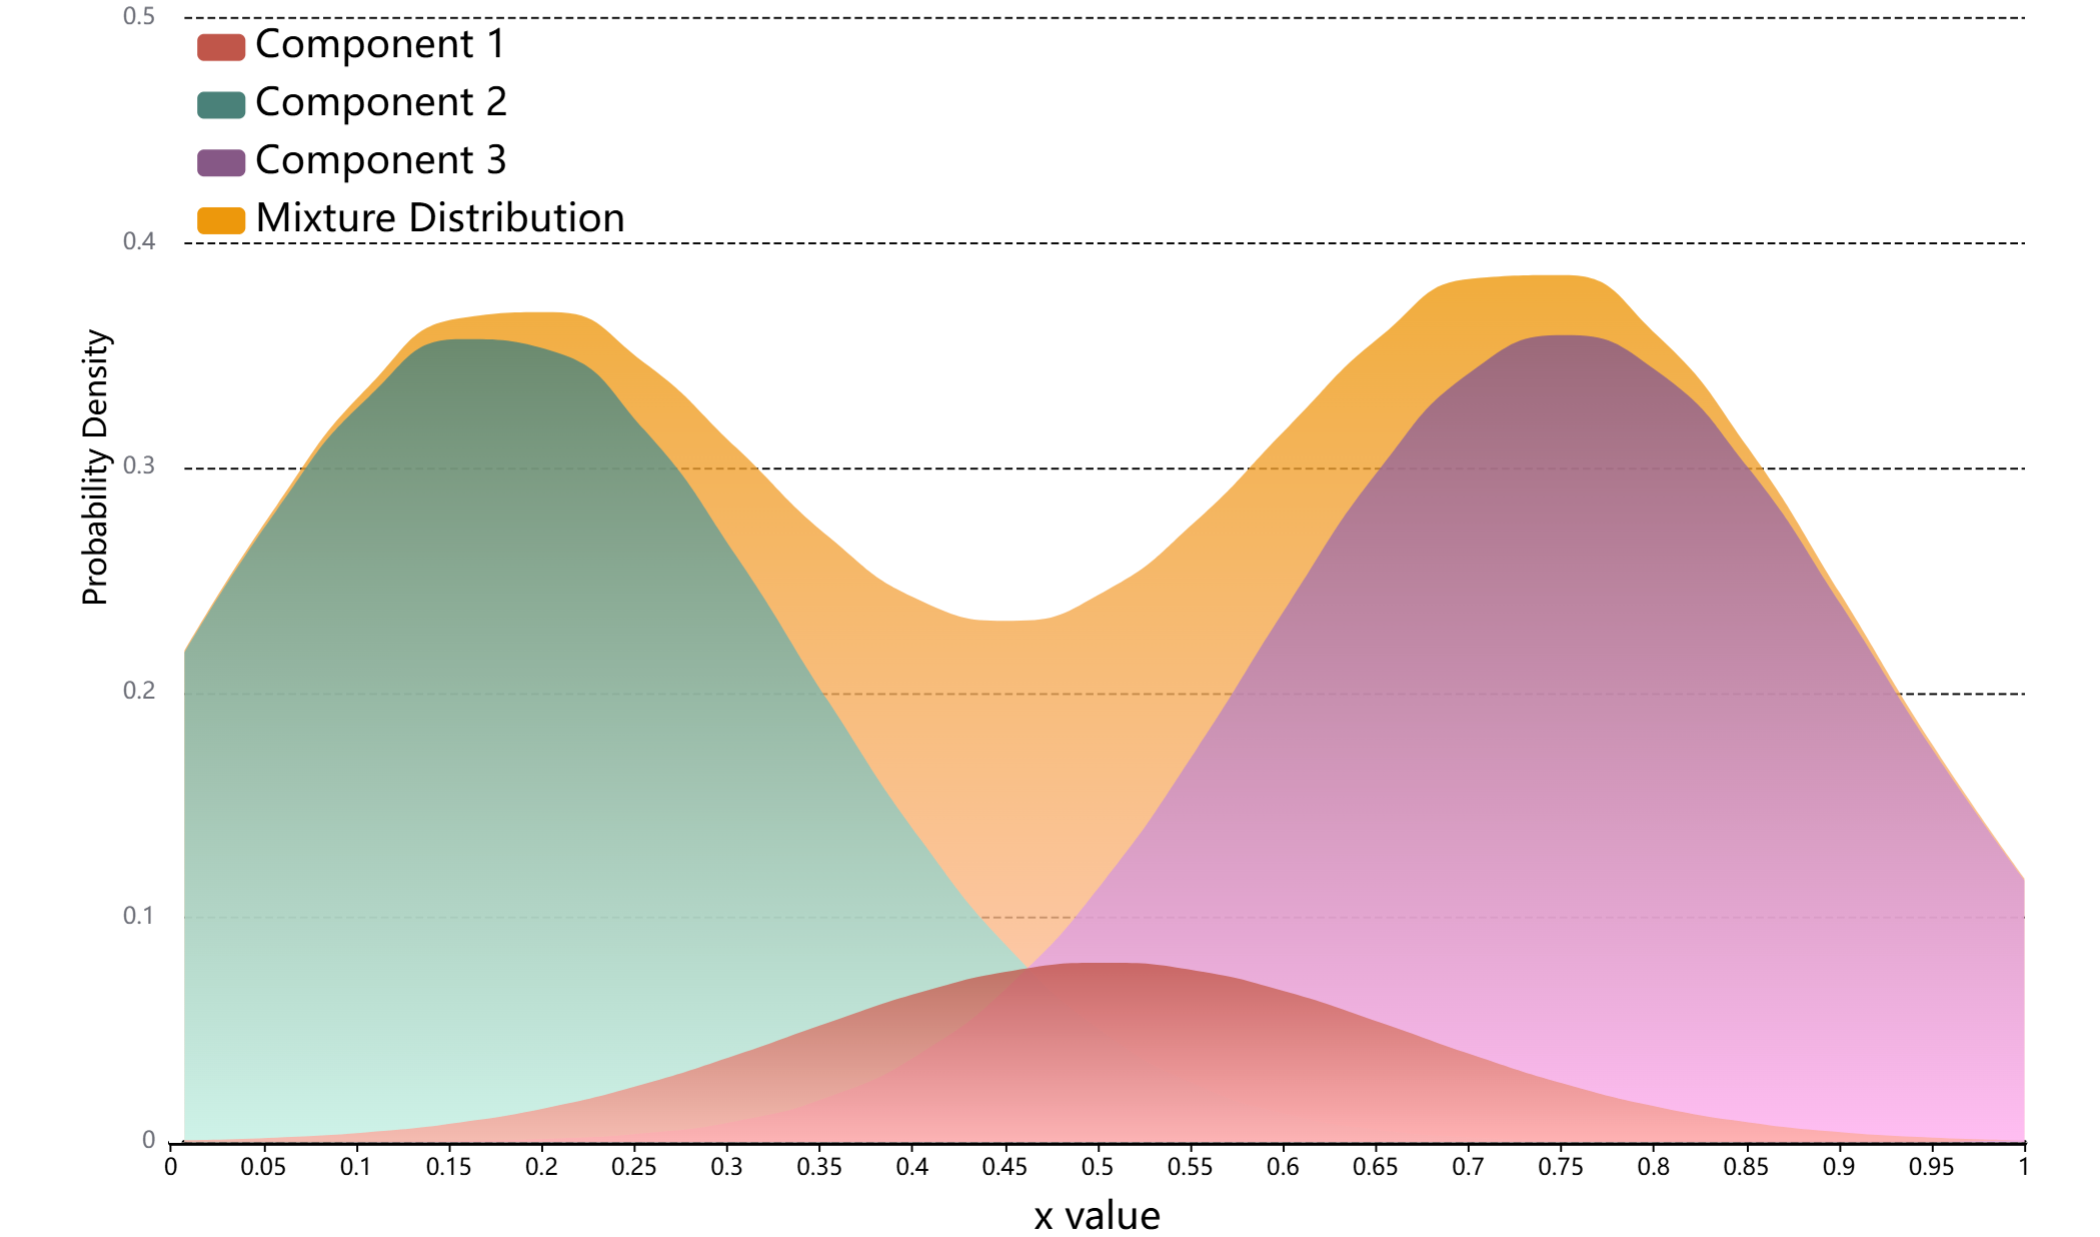
\includegraphics[width=0.4\textwidth]{美赛Latex模板/bb95beeac48592683e1a0f9cdf68773d.png}}% 子图3的相对位置
	\subfigure[Side by side]{				% 图片4
		\label{fig:twob}						% 子图4的标签
		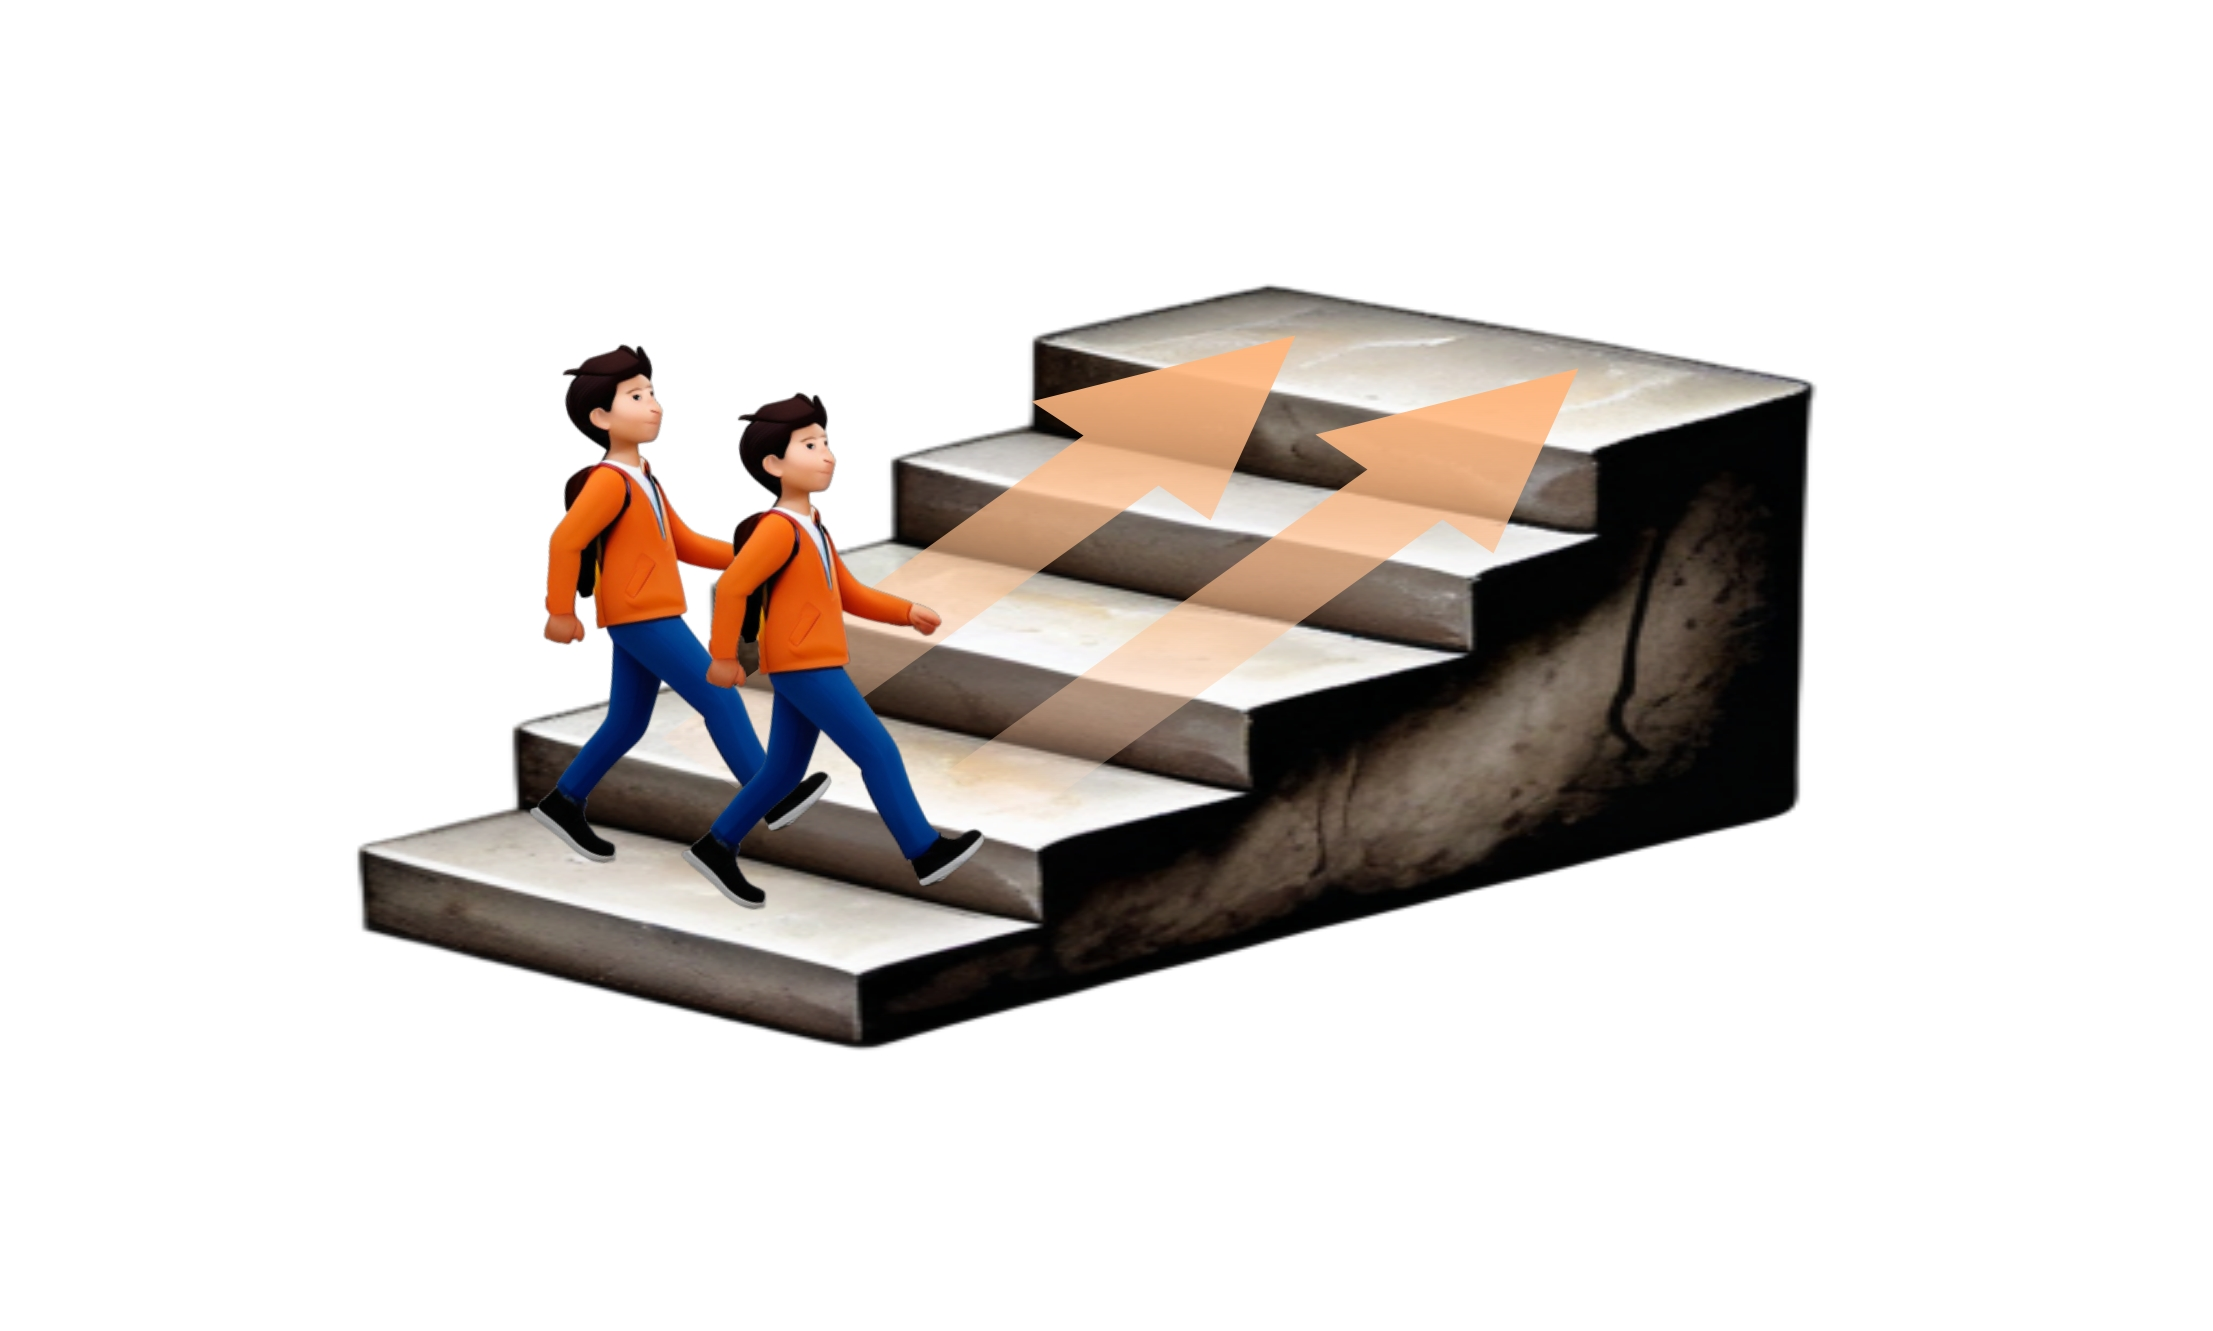
\includegraphics[width=0.4\textwidth]{美赛Latex模板/并行.jpg}}% 子图4的相对位置
	\caption{Distribution of wear in the X-direction and the corresponding number of people}		% 总图标题
	\label{fig:X-two}									% 总图标签
    \vspace{-1.0em}
\end{figure}

The distribution describes how many people used the stairs simultaneously. The number of peaks is the number of people in parallel. In \autoref{fig:X-two}, we give some possible results for archaeologists as a reference: 
\begin{enumerate}[\bfseries 1.]
	\setlength{\parsep}{0ex} %段落间距
	\setlength{\topsep}{-1ex} %列表到上下文的垂直距离
	\setlength{\itemsep}{0ex} %条目间距
	\item When $i=1$, there is only one peak in the x-direction. It can be concluded that people using this stair preferred traveling single files. 
	\item When there are two peaks in the X-direction($i=2$), pairs of people climb the stairs side-by-side.  
	%\item Some small peaks may appear in the results. We consider this to be caused by people walking at different times of the day. It is not considered to be generated in parallel.
\end{enumerate}
\subsubsection{Wear Distribution Model}
Since the lateral position of a footstep on a stone step is not significantly correlated with its longitudinal position, we consider the covariance matrix of the wear distribution to be a diagonal array. For a stone step, we model the wear distribution as follows:
\begin{equation}
    D(x,y)=D_X\cdot{D_Y}
\end{equation}

We compute the actual wear matrix $D^{measure}(x,y)$ obtained from the archaeologist's measurements. Then, we can get its marginal distribution function:
\begin{equation}
    D_X^{measure}(x)=\sum_y{D^{measure}(x,y)}
\end{equation}
\vspace{-1.0em}
\begin{equation}
    D_Y^{measure}(y)=\sum_x{D^{measure}(x,y)}
\end{equation}
With these two edge functions, we can fit $D_x$ and $D_y$, which will help archaeologists obtain relevant information, such as people's traffic patterns.
\vspace{-1.0em}
\subsection{Stair Wear Model}
\subsubsection{Parameters to Be Measured}
 \vspace{-1.0em}
Archaeologists are needed to carry out non-destructive measurements and access information to obtain accurate information and implement the model's solution. We provide the necessary parameters and suggest some measurement methods. It Is shown in Table \ref{parametertable}:

\begin{table}[H]
    \centering
    \vspace{-1.0em}
    \caption{Parameter need to be measured}
    \vspace{-1.0em}
        \begin{figure}[H]
    	\centering
    	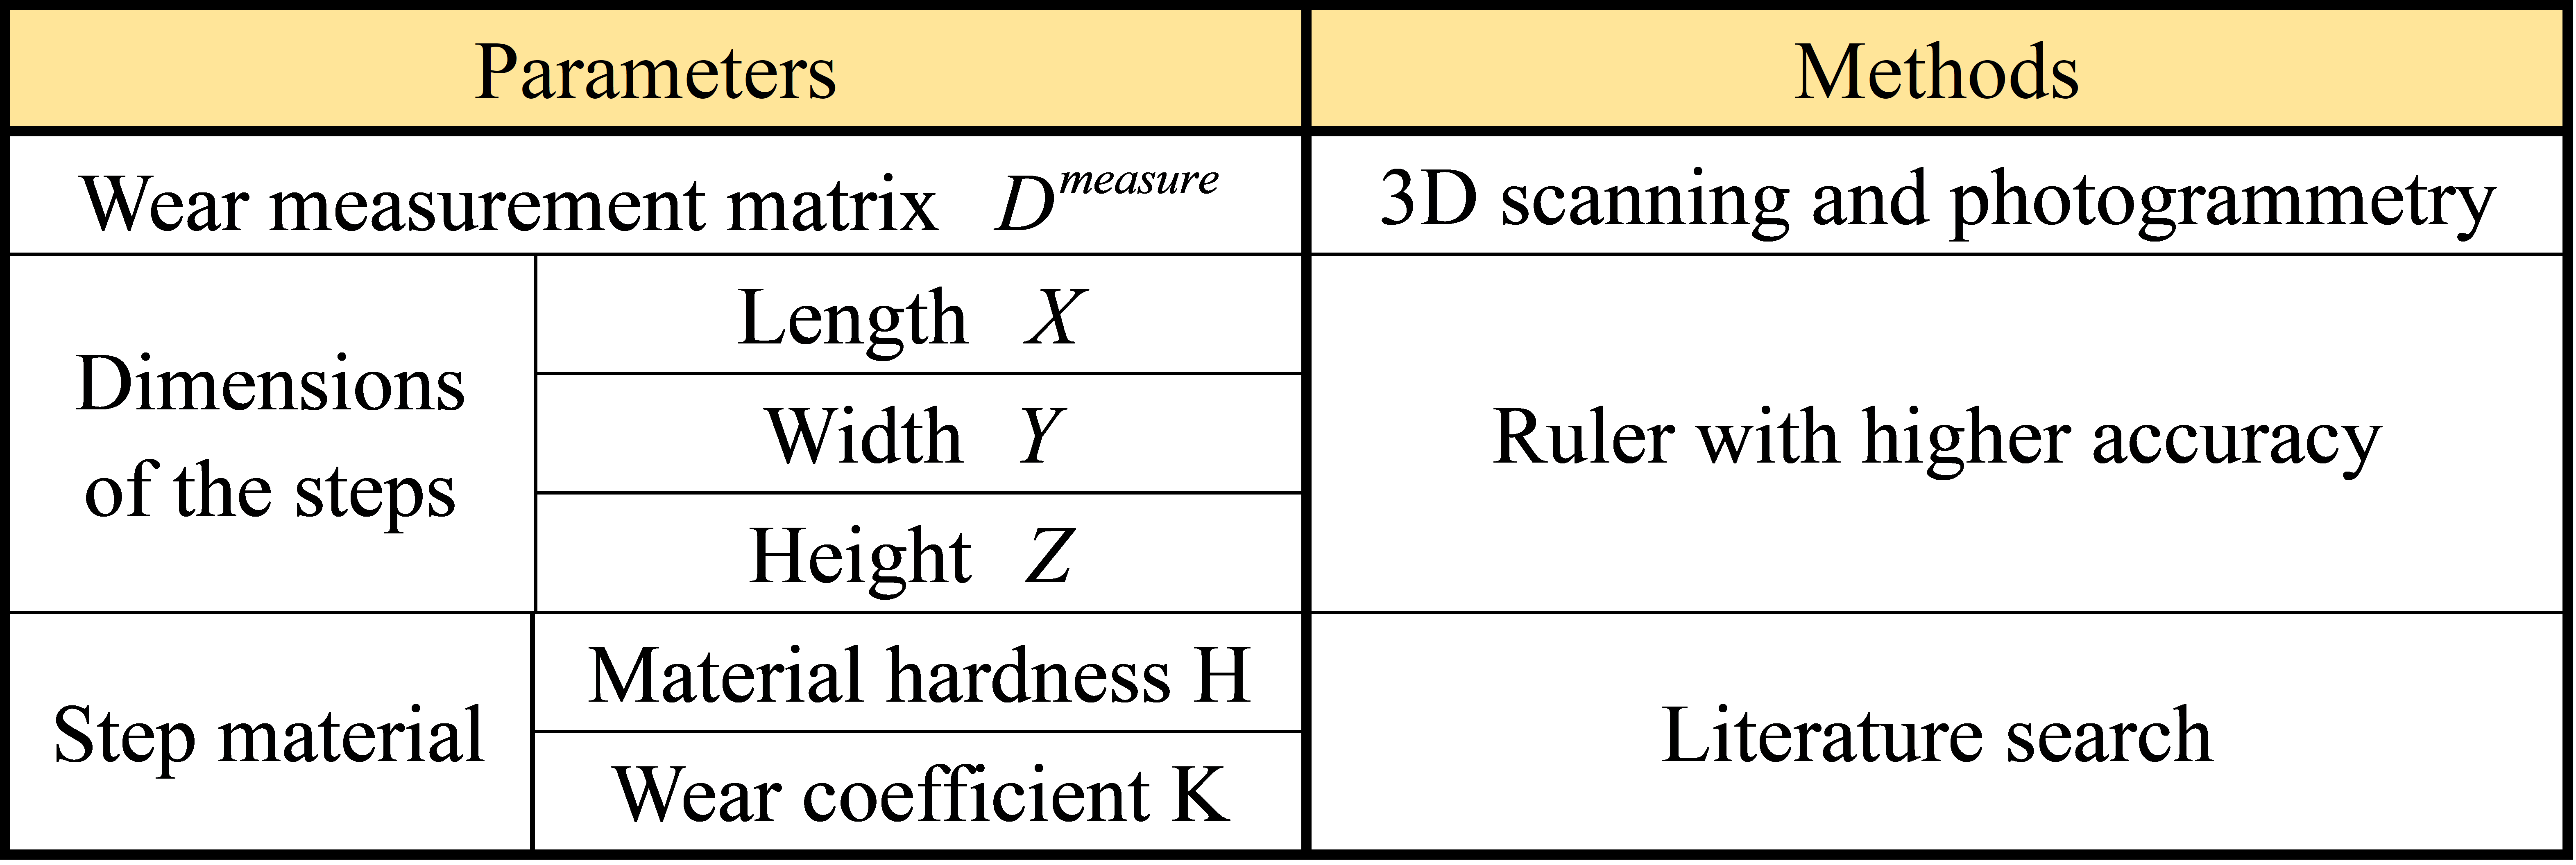
\includegraphics[width=0.8\linewidth]{美赛Latex模板/parametertable.png}
        \end{figure}
    \label{parametertable}
\end{table}

\vspace{-2.0em}

We consider all the methods that require minimum cost, fewer people, and the fewest tools.
\subsubsection{Overview of Stair Wear Model}
Based on the analysis above, the\textbf{ Stair Wear Model }is concluded as below:

\textbf{Wear Volume Model(WVM):}\\
\begin{equation}
\begin{aligned}
    & d_{avg} = \frac{1}{A_{ceff}}\int_{A_{ceff}} T\cdot{N_d}\cdot{D(x,y)}\cdot{G}\cdot{k_m}dxdy\\
    & G=\sum_{i}u_i\cdot{p_i}\\
    & k_m = K\cdot{\frac{d}{H}}\\
    & H(t)=H_0⋅e^{{-}{pt}}\\
    & {H}{T}=\int_{t}H(t)\\
\end{aligned}
\label{MVM}
\end{equation}

\textbf{Wear Distribution Model(WDM):}\\
\begin{equation}
\begin{aligned}
    & D(x,y)=D_X\cdot{D_Y} \\
    & D_{x}\sim w_i\sum_{i}N_i(\sigma_i,\mu_i)\\
    & D_{y}\sim w_{up}\cdot 
      N_i(\mu_{up},\sigma_{up})+w_{down}\cdot N_i(\mu_{down},\sigma_{down})\\
    & D_X^{measure}(x)=\sum_y{D^{measure}(x,y)}\\
    & D_Y^{measure}(y)=\sum_x{D^{measure}(x,y)}
\end{aligned}
\label{WDM}
\end{equation}
All parameters have been explained above.
In order to show our model more clearly and to make it easier for archaeologists to understand it, we give the flow chart for use in \autoref{flowchart_Experts}:
\begin{figure}[H]
	\centering
 	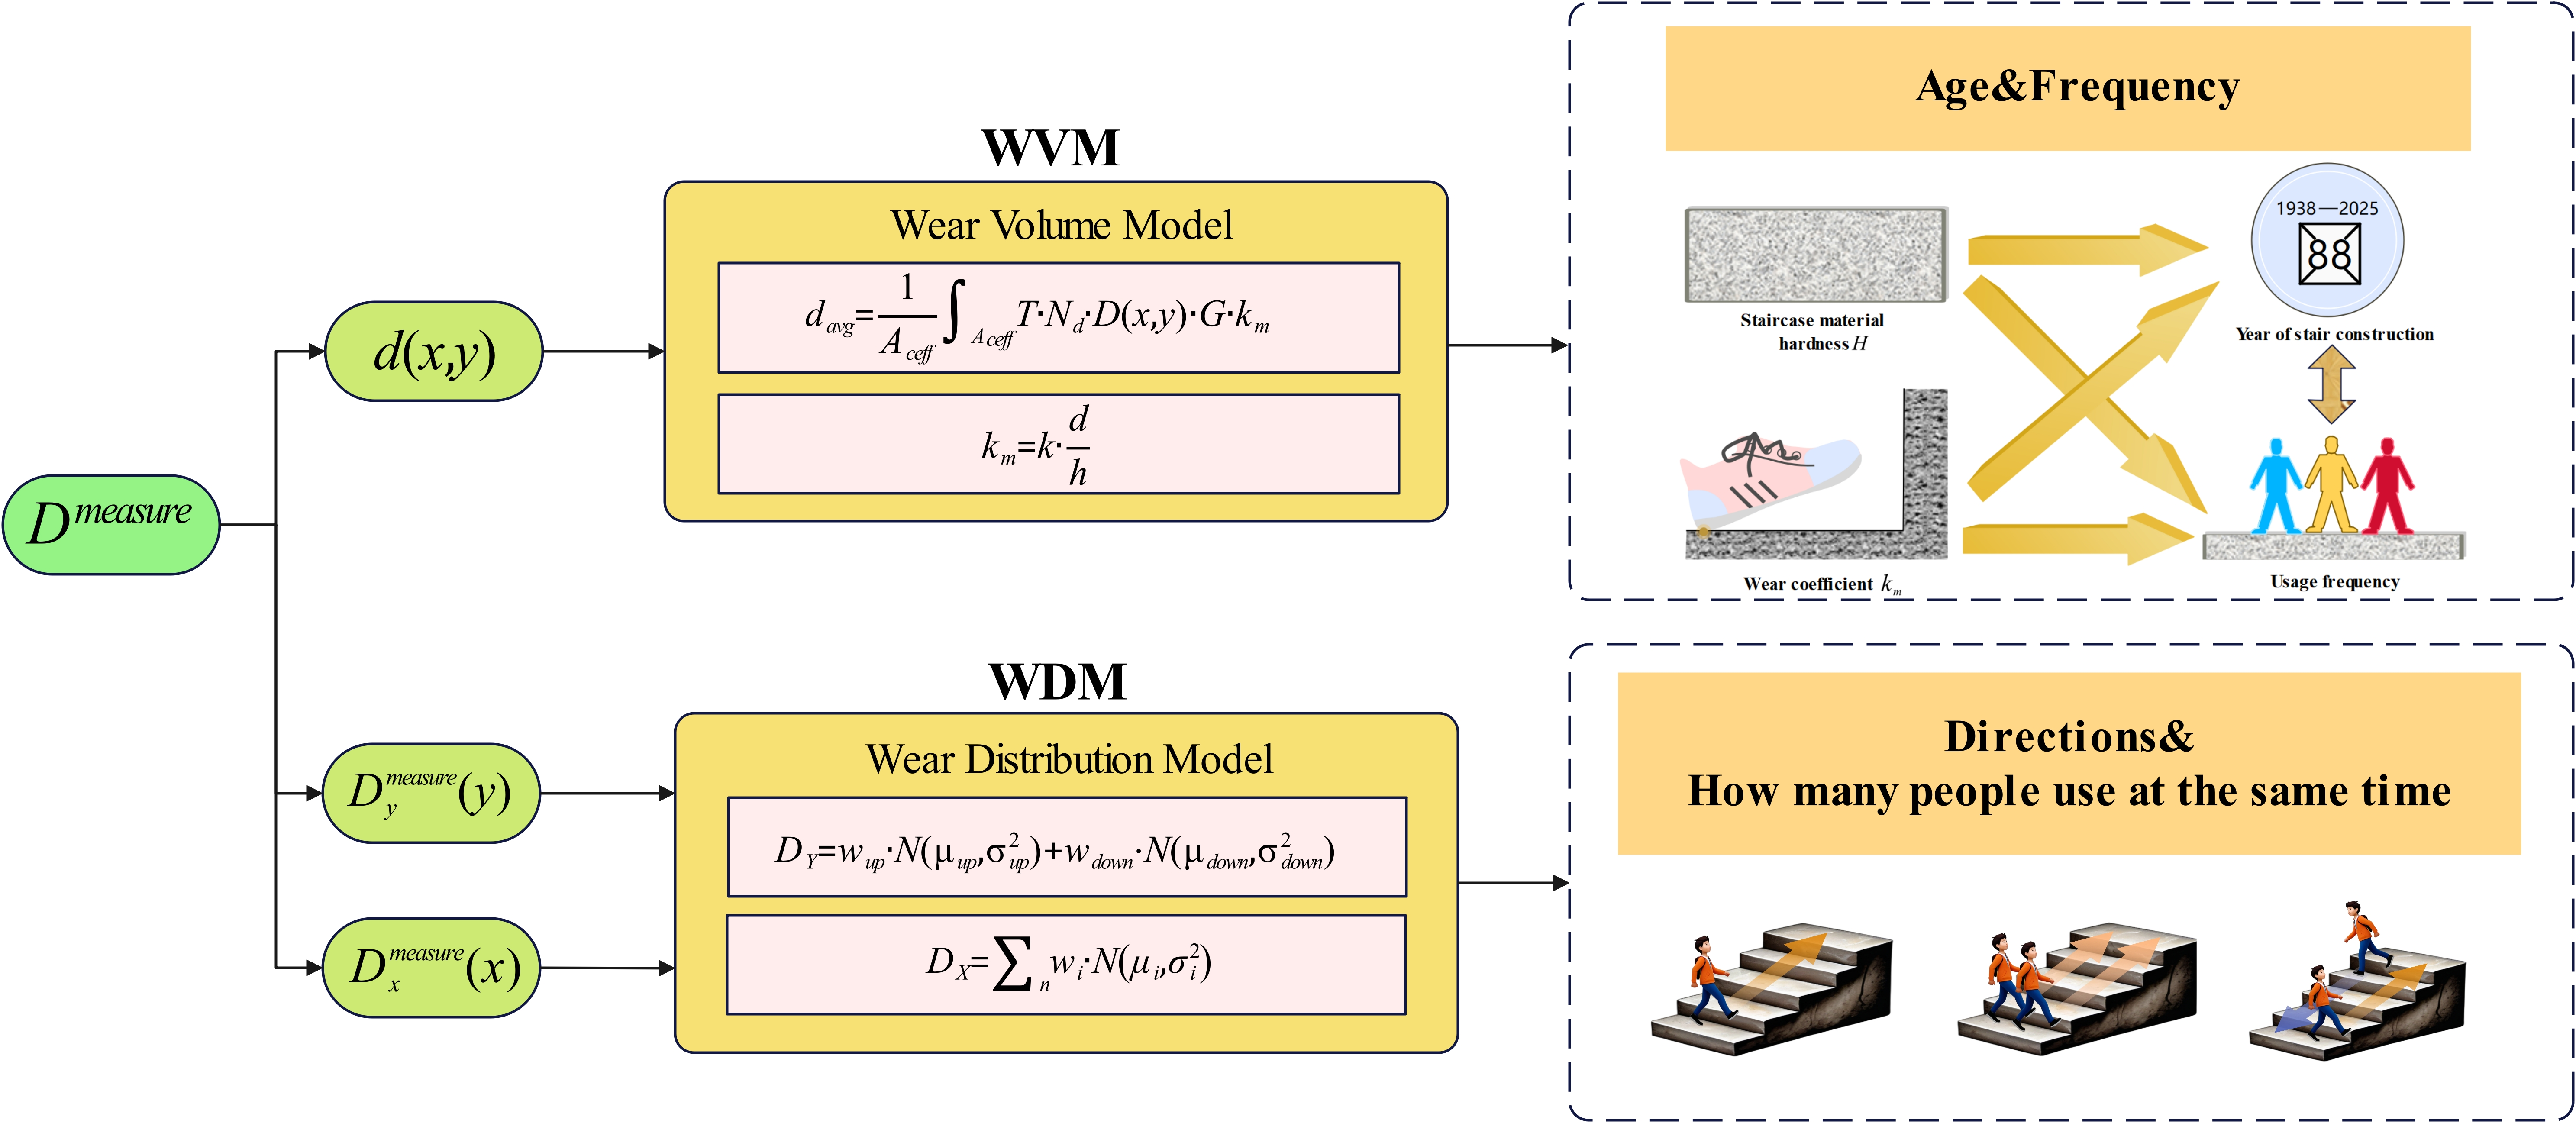
\includegraphics[width=\linewidth]{美赛Latex模板/模型流程图1.jpg}
	\caption{Flowchart for use by archaeological experts}
	\label{flowchart_Experts}
\end{figure}

\subsection{Solution of the Stair Wear Model}
In this section, we selected a set of ancient Edinburgh sandstone steps with a rectangular top-view surface. The rectangle is 2 meters long and 0.4 meter wide. Based on the 3D reconstruction of the image, we obtained the measurement matrix. Moreover, based on the information query, we obtained the rest of the required parameters as follows:
\begin{table}[H]
    \centering
    \caption{Key Parameters}
            \renewcommand{\arraystretch}{1.5}
        \setlength{\tabcolsep}{16pt}
    \label{tab:keyparameters}
    \begin{tabular}{lcc}
        \hline
        \textbf{Parameter} & \textbf{Value} & \textbf{Unit} \\
        \hline
        $G$ & 700 & N \\
        $K$ & $1.8 \times 10^{-7}$ & (dimensionless) \\
        $d$ & 0.8 & mm \\
        $H$ & 95 & N/mm\textsuperscript{2} \\
        \hline
    \end{tabular}
\end{table}

To solve the Wear Distribution Model, we design a Gauss Mixtual Algorithm. It can be used to respectively solve for normally distributed cumulants in the X and Y directions by wear measurement matrix $D^{measure}$. The exact flow of the algorithm is as follows:

\begin{table}[H]
    \centering
    \renewcommand{\arraystretch}{1.5}
    \setlength{\tabcolsep}{16pt}
    \begin{tabular}{>{\raggedright\arraybackslash}p{15cm}} 
        \hline
        \textbf{Gauss Mixtual Algorithm}\\ 
        \hline
        \textbf{Input:}\quad Wear measurement matrix $D^{measure}$\\  %Length $X$, Width $Y$?
        \textbf{Output:}\quad $P(D_X\mid\theta_k^{epoch})$ and $P(D_Y\mid\theta^{epoch})$ \\
        \(k = 0\) , \(\varepsilon = 1e-3\)\\
        while \(loss>\varepsilon\)\\ 
        \qquad for \(t\) in range($epoch$)\\ 
       \qquad\qquad \(\theta^{t+1}=\theta^{t}-
{\partial P(D_X\mid\theta^{t})}/{\partial \theta^t}
\), where $\theta=[ m_i,\mu_i,\sigma_i ]$\\
       \qquad\qquad $P(D_X\mid\theta^{t+1})=\sum_{i=1}^{k}m_i^{t+1}\cdot{N(\mu_i^{t+1},\sigma_i^{t+1})}$\\
      \qquad $loss = \Vert P(D_X\mid\theta_k^{epoch})-D_X \Vert$ \\

\(k = 2\)\\
for \(t\) in range($epoch$)\\ 
       \qquad \(\theta^{t+1}=\theta^{t}-
{\partial P(D_Y\mid\theta^{t})}/{\partial \theta^t}
\)\\
    \qquad $P(D_Y\mid\theta^{t+1})=m_{up}^{t+1}\cdot{N(\mu_up^{t+1},\sigma_up^{t+1})}+m_{down}^{t+1}\cdot{N(\mu_down^{t+1},\sigma_down^{t+1})}$\\
       end\\
        \hline
    \end{tabular}
    \vspace{-0.8em}
\end{table}
Bringing $D^{measure}$ of the  Edinburgh sandstone step into the Gauss Mixtual Algorithm, we obtain the following normal distribution parameters. The parameters for the X and Y directions are placed in Table \ref{X_TABLE} and Table \ref{Y_TABLE} respectively.

\vspace{-3em}
\begin{minipage}[t]{0.5\linewidth}%第一栏尺寸
        \begin{table}[H]
    	    \centering
            \caption{\centering Normal distribution parameters in X direction}
            \vspace{-1em}
            \begin{figure}[H]
        	\centering
        	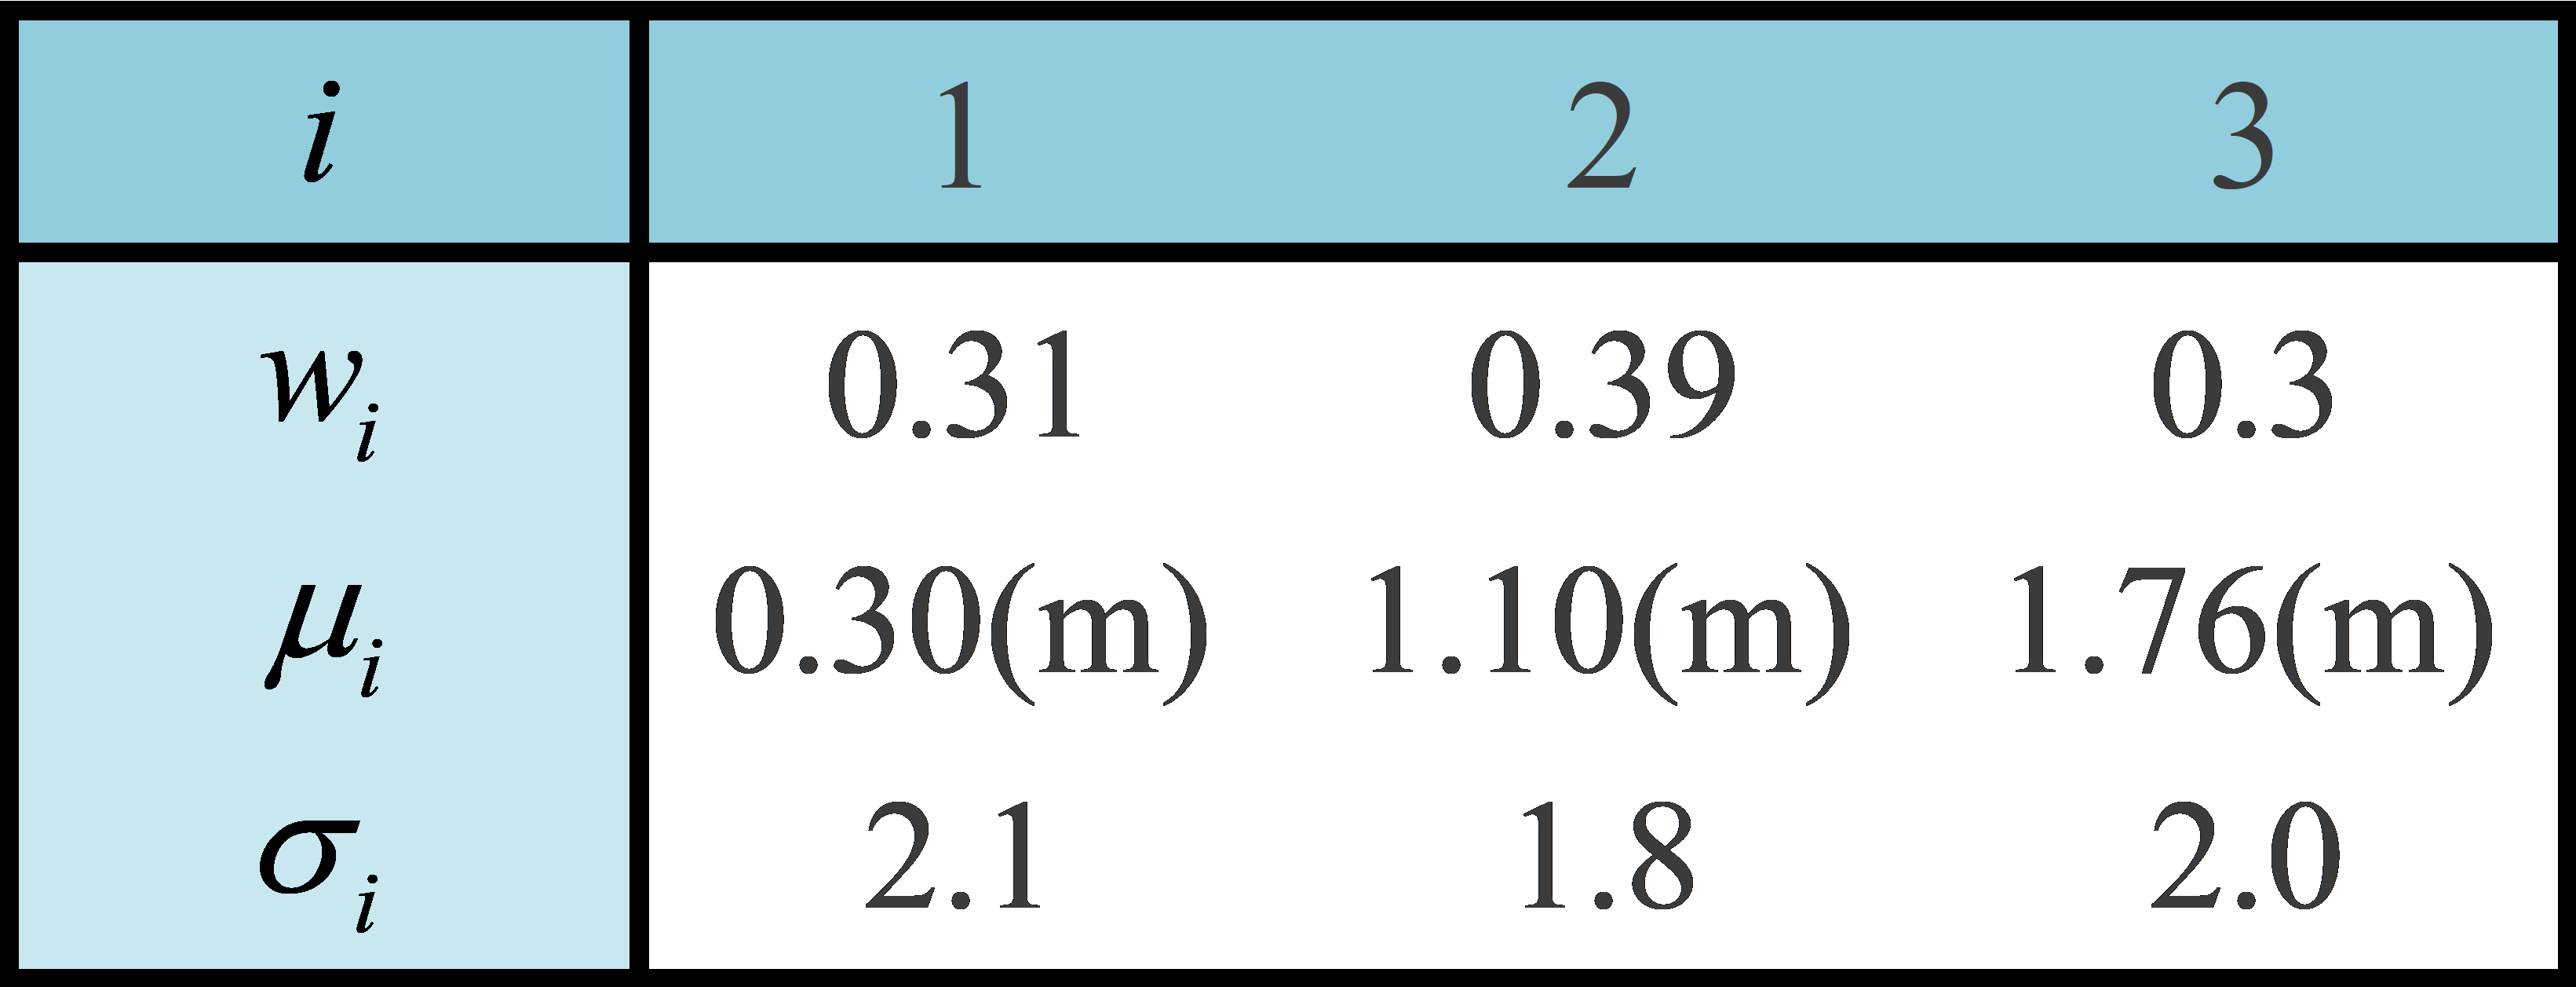
\includegraphics[width=0.8\textwidth]{X_TABLE.png}
        \end{figure}
        \label{X_TABLE}%设置专属标签,方便引用
        \end{table}
    \end{minipage}%第一栏结束
    \begin{minipage}[t]{0.5\linewidth}%第二栏尺寸
        \begin{table}[H]
    	    \centering
            \caption{\centering Normal distribution parameters in Y direction}
            \vspace{-1em}
            \begin{figure}[H]
        	\centering
        	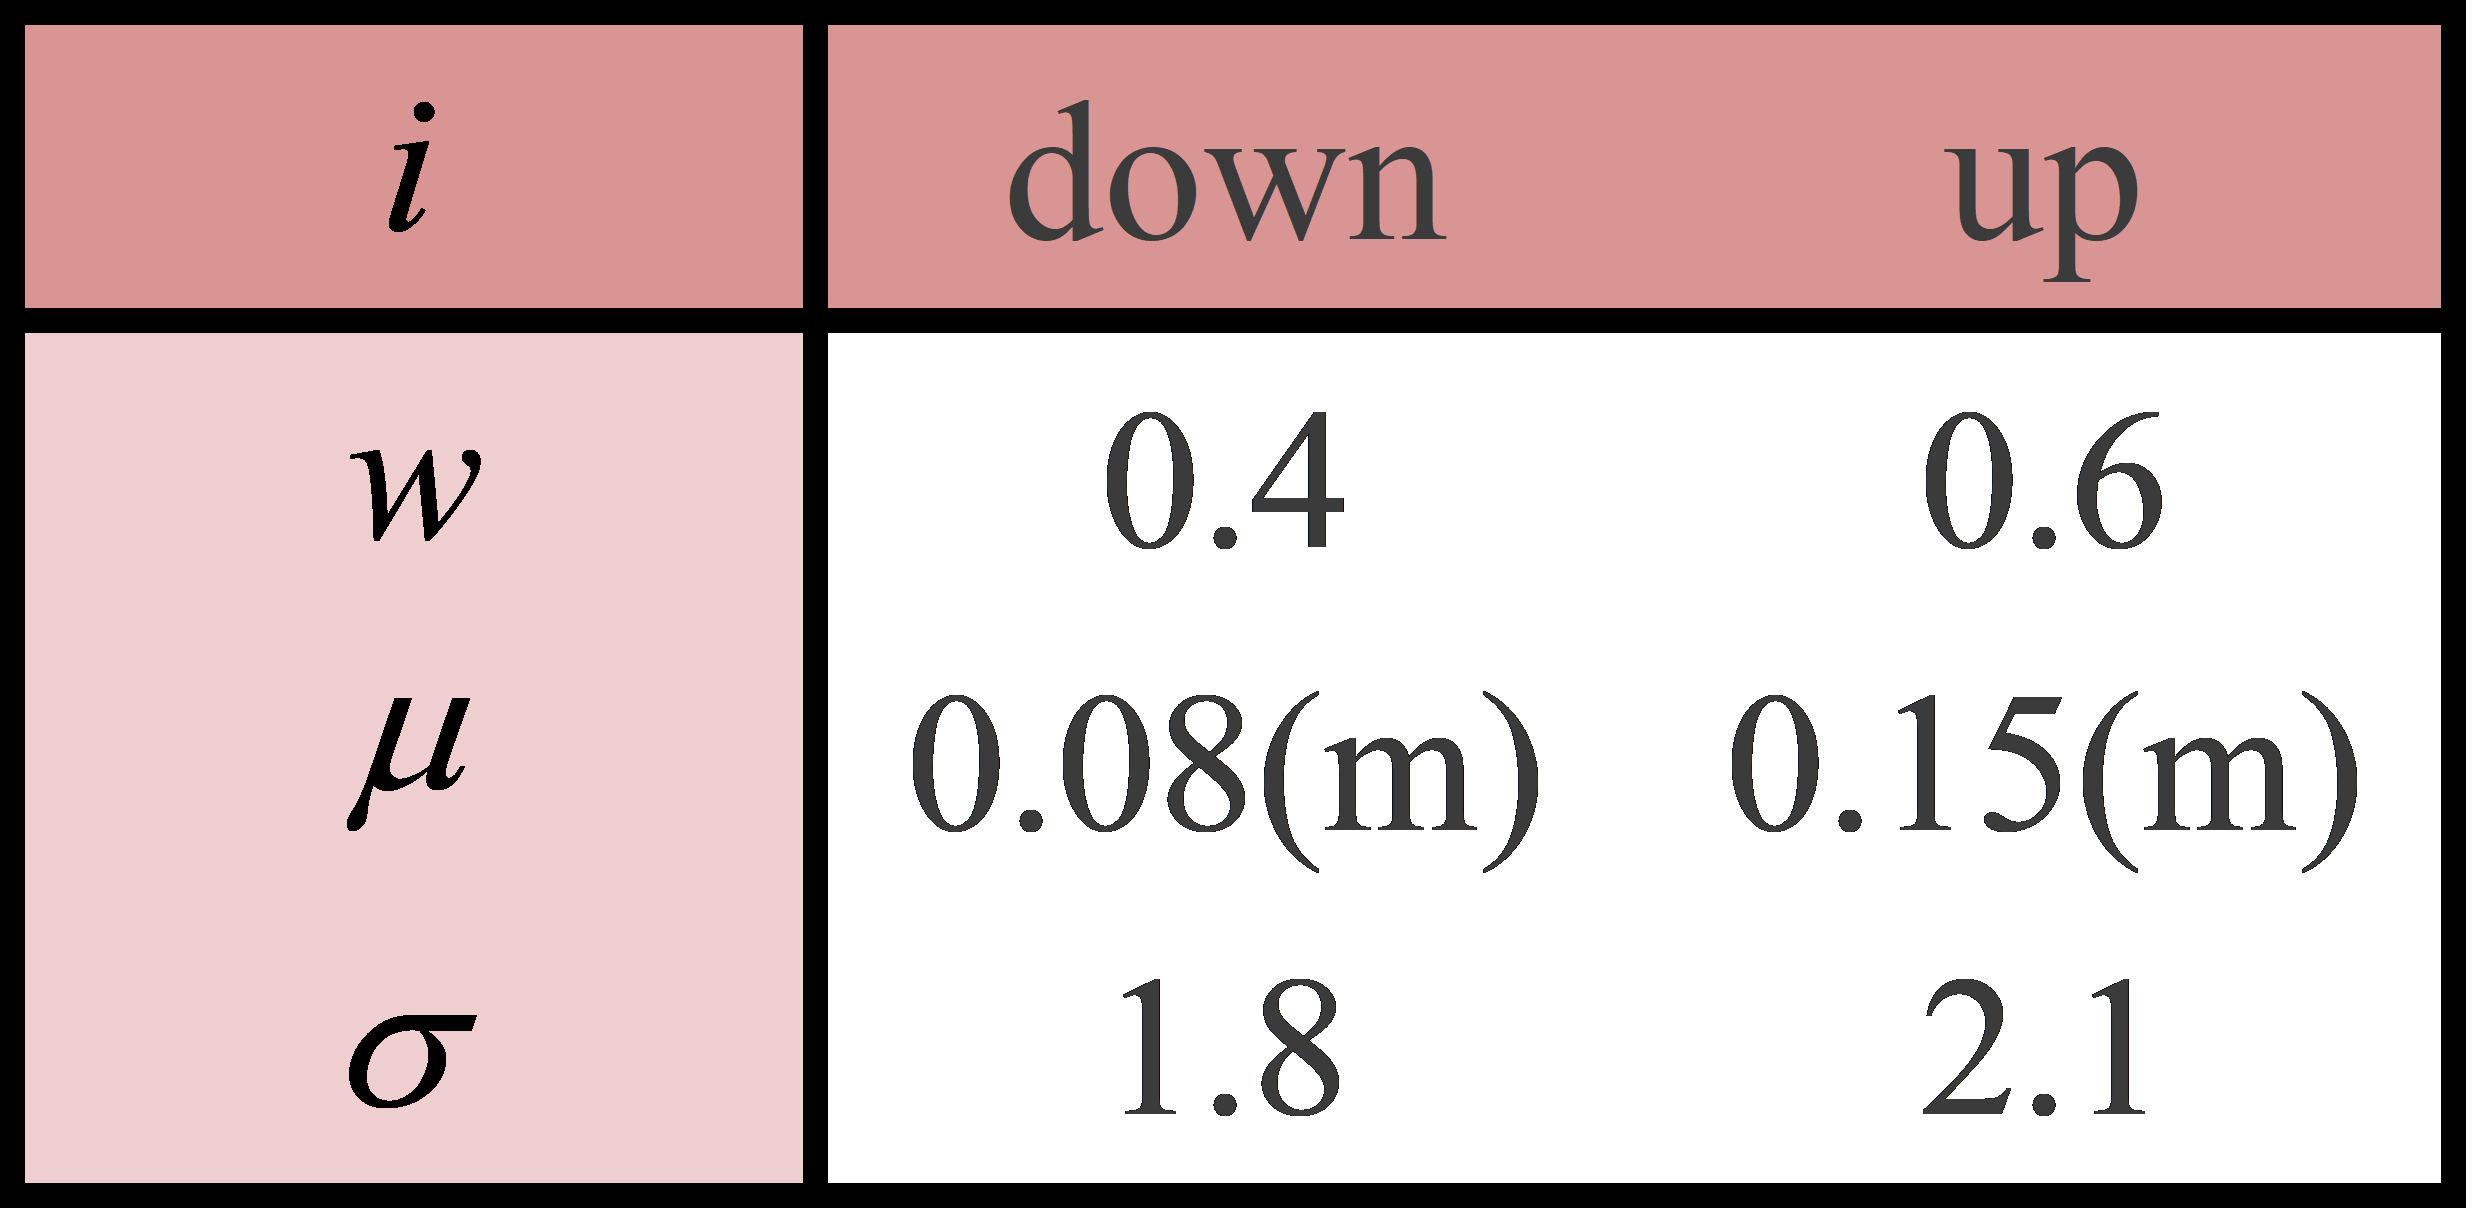
\includegraphics[width=0.6\textwidth]{Y_TABLE.png}
        \end{figure}
        \label{Y_TABLE}%设置专属标签,方便引用
        \end{table}
         \vspace{-2em}
    \end{minipage}\par %第二栏结束

From  Table \ref{X_TABLE} and Table \ref{Y_TABLE}, we can draw the conclusions that
\begin{enumerate}[\bfseries 1.]
	\setlength{\parsep}{0ex} %段落间距
	\setlength{\topsep}{-1ex} %列表到上下文的垂直距离
	\setlength{\itemsep}{0ex} %条目间距
	\item The wear distribution in the X-direction is accumulated from three normal distributions. The mean values of the three normal distributions are 0.30m, 1.10m and 1.76m. They are respectively on the left, centre and right side of the step. This reveals that \textbf{three people usually walked side by side on this step}. This may also show that the stair had a high flow of people.
	\item Of the three normal distributions in the x-direction, the second one has the highest probability and the smallest standard deviation. This indicates that people most often walked down the \textbf{middle} of the stairs. 
	\item Two normal distributions form a wear distribution in the Y-direction. \textbf{The stair was used in two direction}. The probability ratio of the number of people in the upward and downward direction was \textbf{3 : 2}. 
 %The standard deviation of the normal distribution corresponding to the upward direction is larger than that of the downward direction. 
 It means that the number of people in the \textbf{upward} row is \textbf{greater} than the number of people in the \textbf{downward} row.
     \item The mean of upward direction is 0.08m, while that of downward direction is 0.15m. They both close to the edge side of the step. Moreover, the mean of upward direction is closer to the edge of the step than the downward direction. This is consistent with our analysis.
\end{enumerate}
\vspace{-1em}

To describe the results of this set of steps more intuitively, we visualize the wear distribution of the steps and present them in \autoref{stepwear3}.
\begin{figure}[H]
\vspace{-1em}
	\centering
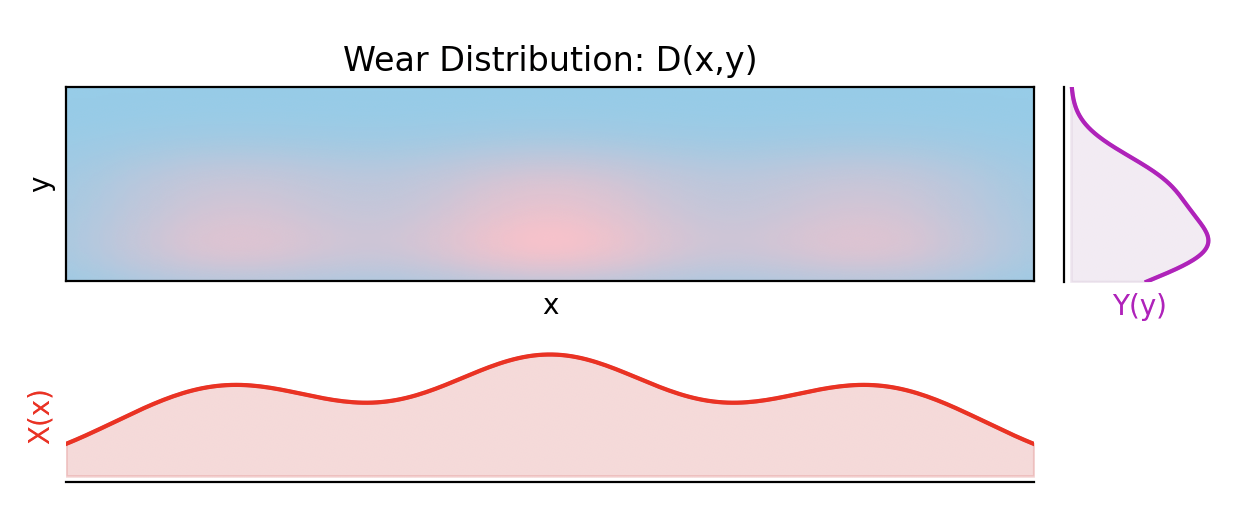
\includegraphics[width=0.8\linewidth]{美赛Latex模板/stepwear3.png}
	\caption{Visualization of step wear distribution}
	\label{stepwear3}
 \vspace{-1em}
\end{figure}
This graph gives the same conclusions. It visually presents three peaks in the X-direction, indicating that people usually walked side-by-side on it. There are two peaks in the Y-direction. The peak corresponding to the downward direction is smaller than that of the upward direction. This suggests that the staircase was used in a double direction.

After obtaining the wear distribution, combined with the parameters in Table \ref{tab:keyparameters}, the gradient age and frequency of use can be solved for each other. For this set of ancient Edinburgh sandstone steps, it is determined that this set of steps was constructed in a century ago. according to \autoref{MVM}, we can have that 
\begin{equation}
     N_d = \frac{A_{ceff}\cdot{d_{avg}}}{T\cdot{G}\cdot{k_m}}=261
\end{equation}
 This means that \textbf{261 people} walked on it every day in the past. On the contrary, when we consider that 260 people walked on it per day, the steps were constructed \textbf{36492} days ago.


\section{Further Problems}
In this section, we propose solutions and computational models for the further problems.
\subsection{Consistency of Wear Results}
According to the available information, we can get a more accurate wear distribution matrix $D^{available}$. To judge whether the wear is consistent with the information available is to judge the consistency of $D^{available}$ and $D^{measure}$. We define the following consistency formula:
\begin{equation}
    PA = D^{available}(x, y) \sum_x \sum_y \log \left( \frac{d^{ava}(x, y)}{d(x, y)} \right)
\end{equation}
$d^{ava}(x,y)$ is the amount wear depth of the stone step on the grid where each COP is located. and $d(x,y)$ is that of the actual measured.  $PA$ is a number greater or less than 0. The greater the absolute value $PA$, the weaker the correlation between the two matrices.
\subsection{The Age of The Stairwell and Reliability}
In Section 3, we give the method of estimating the age of each step. For a given stair, we measure the ages of all steps and find them different. When the difference is slight, it is mainly because the model has errors. However, when the difference is significant, it is due to refurbishment or repairs that cause the individual steps to age differently. In a stairwell, if the age of a step is 5\% less than the age of the largest step $T_{lar}$, it is removed. The average age of the remaining steps as the age of the stairwell $T_{set}$. It can be expressed as
\begin{equation}
   T_{set}= \overline{T_i},\quad\frac{T_i}{T_{lar}}>0.95
\end{equation}
There are $N$ steps in tatal. $T_i$ is the age of step $i$, $i=1,2,\cdots,N$. 

Age reliability is necessary to be assessed. We estimate the ages of $n$ ancient stone stairs in total. If the error between the result and the real age is within 5\%, RA is accepted and included, otherwise RC is included. The age reliability $CI$ is defined as:
%可靠性公式
\begin{equation}
   CI_{inf} = {\left[ 1 + \frac{RC + 1}{RA\cdot F_{1-\alpha/2}(2RA, 2(RC+ 1))} \right]}^{-1}
\end{equation}
\begin{equation}
   CI_{sup} = {\left[ 1 + \frac{RC}{(RA+1)\cdot F_{1-\alpha/2}(2(RA+1), 2(RC))} \right]}^{-1}
\end{equation}
where $\alpha=0.05$. 

We studied 6 Edinburgh sandstone steps living more than one century and calculated that 5 of which have an error within 5\%, which means we can say the age reliability is between 0.359 and 0.996

\subsection{Repairs or Renovations }
Two methods are proposed to find out which steps have been repaired or refurbished.

\textbf{Method 1: Step Age Method}

\textbf{Brief Introduction:} Measure the age of each step by the Stair Wear Model and compare them.

According to Assumption 4, each step is trampled at the same frequency. Therefore, in the absence of repairs or renovations, the age of all the steps should vary slightly. The correlation degree $RSA$ between step $i$ and the whole is defined as:
\begin{equation}
    RSA = \min_{i} \frac{T_i}{T_{set}}
\end{equation}
$T_i$ is the age of step $i$, and $T_{set}$ is the age of the stair. This coefficient is typically a value between 0 and 1, where higher values indicate greater correlation. When $RSA_k$ is smaller than 0.95, it indicates that the $k$th step has been repaired or renovated. The time of repairs or renovations $T_{re}$ can also be determined by
\begin{equation}
    T_{re} = T_{n}-T_k
\end{equation}
$T_n$ is the year in which the archaeologists began their measurements.  Since there may be errors in the calculation of age, we also provide an alternative method.

\textbf{Method 2: Improved Non-destructive Measurement based on Brinell Scale and KL scatter}

\textbf{Brief Introduction:} Combined with the Brinell scale theory and KL scatter, calculate hardness of each step material by using the existing wear matrix. Compare its consistency to determine which step has been repaired and give the time calculation formula.

Brinell scale is a scale that measures the hardness of a material and is one of the properties of the material. Brinell scale measurement is a way of measuring the hardness of materials. A typical test uses a hardened steel ball with a diameter of $D_p$ mm as an indenter. A force of $F$ is applied to the indenter and held for a certain amount of time. Then the diameter of the indentation caused by the indenter on the surface of the material is measured. The hardness $H_B$ is calculated as follows:
\begin{equation}
    H_{B} = 0.102 \cdot \frac{2F}{\pi D_p \left( D_p - \sqrt{D_p^2 - d_p^2} \right)}
\end{equation}
where $d_p$ = diameter of indentation (mm).

Due to the absence of repairs or renovations, people exert the same continuous pressure on each step of a stair over time. We take the average gravity $G$ as $F$, the average wear depth $\overline{d}$ of the step as the indenter diameter $D_p$, and the square root of the area $\sqrt{A_{ceff}}$ of a step as the indentation diameter $d_p$. At this time, the hardness $H_{test}$ is calculated as follows:
\begin{equation}
    H_{test} = 0.102 \cdot \frac{2G}{\pi {\overline{d}} \left( {\overline{d}} - \sqrt{{\overline{d}}^2 - A_{ceff}} \right)}
\end{equation}
When the $H_{test}$ of each step has a large difference, the step with the larger $H_{test}$ has been repaired. We use the variance $\sigma_H$ to discribe the dispersion of $H_{test}$.


 Even if the Brinell scale is similar and  the materials are consistent , it is possible that it has been repaired. Referring to the KL scatter, we propose a definition of the correlation between two stone steps:
 \begin{equation}
     RS(d_1, d_2) = D_1(x, y) \sum_x \sum_y \log \left( \frac{d_1(x, y)}{d_2(x, y)} \right)
 \end{equation}
 $RS(d_1, d_2)$ is the correlation between the worn volumes of the two stone steps, $D_1$ represents the wear distribution of the comparative stone steps, $d_1(x, y)$ denotes the average wear depth of the corresponding raster of the comparative stone steps, and $d_2(x, y)$ denotes that of the compared stone steps. The similarity threshold is set as $\varepsilon=0.05$. When $|RS(d_1, d_2)|>\varepsilon$, it is considered that the comparative stone step has been repaired. 
 
 Combining $H_{test}$ and $RA$, we can determine which repair or renovation occured in this stair. Moreover, the repair time can be determined as:
 \begin{equation}
     T_{\text{repair}}^{d_1} = T^{d_2} \cdot e^{RS(d_1, d_2)}
 \end{equation}
 where $T_{\text{repair}}^{d_1}$ refers is the length of time from when the stair was built to when the step was repaired, and $T^{d_2}$ denotes the time that the stone steps were built.
 
For the Edinburgh sandstone steps we studied, we calculated that
\begin{enumerate}[\bfseries (1)]
\vspace{-0.5em}
	\setlength{\parsep}{0ex} %段落间距
	\setlength{\topsep}{-1ex} %列表到上下文的垂直距离
	\setlength{\itemsep}{0ex} %条目间距
	\item $RSA=0.02<0.05$
	\item All the $H_{text}$ of steps are close to $89.45N/mm^2$ while $\sigma_H=1.8$
	\item $RS=0.03<0.05$
 \vspace{-0.5em}
\end{enumerate}

\textbf{Therefore, this set of steps has not been repaired or renovated.}

 
 
\subsection{The Source of The Material}
As analyzed in Section 4.3, we can determine the type of materials to a certain extent through the Brinell scale. In our model, $H_0$ denotes Brinell scale. Therefore, according to the Wear Volume Model (\ref{MVM}), the average quantity of $H$ over a time scale, $H_t$, can be obtained, which can be expressed as:
\begin{equation}
    H_t = \frac{N_d \cdot G \cdot T \cdot K \cdot d}{d_{\text{avg}} \cdot A_{\text{ceff}}}
    \label{eq:Htest}
\end{equation}
$N_d$ indicates the stair use frequency, $G$ denotes the average gravity, $T$ indicates the stair age, $K$ is the material wear coefficient, $d$ is the average wear distance, $d_{avg}$ is the average measured wear depth, and $A_{ceff}$ is the area of the step.

People have studied numerous kinds of materials deeply. Here we demonstrate sevearl Brinell scale ($H_0$)for four commonly used steps\cite{4}\cite{5}:
\begin{table}[H]
    \centering
    \vspace{-0.5em}
    \caption{Hardness of different materials}
    \vspace{-1.0em}
        \begin{figure}[H]
    	\centering
    	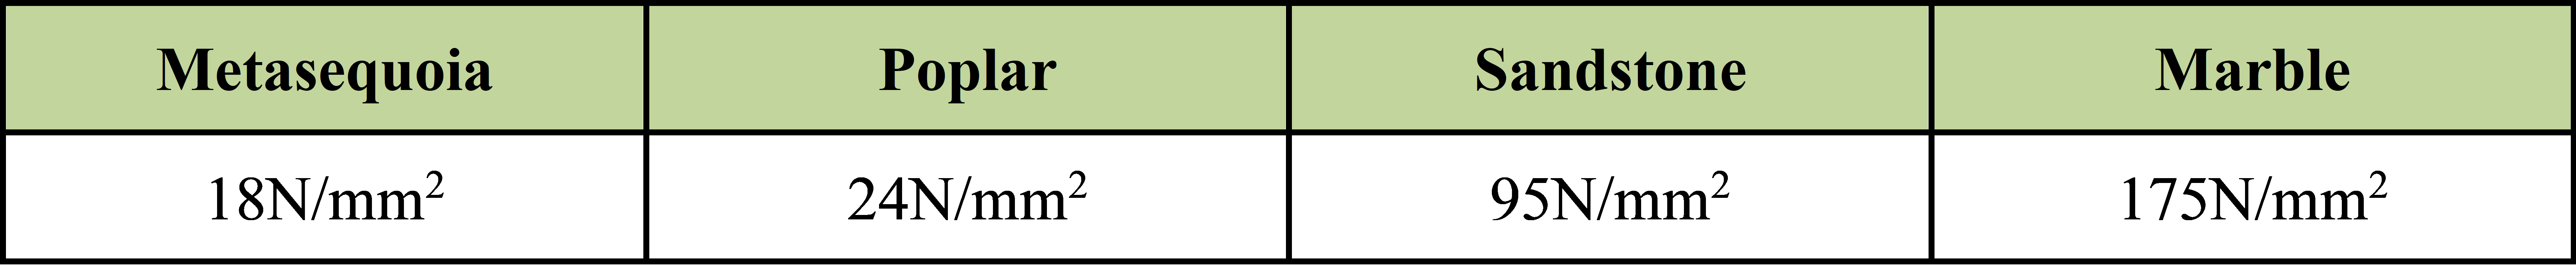
\includegraphics[width=0.8\linewidth]{KindsofH.png}
        \end{figure}
    \label{differentH}
    \vspace{-2em}
\end{table}


We can refer to available data to obtain the Brinell scale $H_{0A}$ of the material we considered to be the origin, calculating its average $H_{0At}$ over time according to \eqref{eq:HT}. Then its agreement with the model theoretical value $H_t$ can be obtained by:
\begin{equation}
    \eta = \frac{\left| H_{t} - H_{0At} \right|}{H_{0At}} \cdot 100\%
\end{equation}
If $\eta<0.05$, we believe that we successfully determine the origin. For instance, considering the Edinburgh steps we studied. It is said to be constructed by sandstones. According to the literature, We know that the Brinell scale $H_0$ of standard sandstone is $95\text{N/mm}^2$. It can be calculated that $H_t =90.44\text{N/mm}^2$. $H_{0At} = 93.18$. Therefore, $\eta = {\left| H_{t} - H_{0At} \right|}/{H_{0At}}=0.030 $. We can confirm its origin.

Refering to the analysis of rock, we give the hardness attenuation formula of wood:
\begin{equation}
    H(t) = H_0 \cdot e^{-(0.0015 \cdot T + 0.02 RH) \cdot t}
\end{equation}

Unlike stone, the hardness of wood is also influenced by its age when used for constructing stairs. Its age can potentially be determined from the growth rings visible on the stairs.



To determine whether the wear is consistent with materials from the quarry the archaeologist believes to be the original source. We need to perform the same simulation on the raw materials based on the available information. For instance, we set the same environment for the steps of these four materials in \autoref{differentH}. People's walking pattern is constructed by the normal distribution parameters in \autoref{X_TABLE} and \autoref{Y_TABLE}. Except $H_0$, other parameters in Table \ref{tab:keyparameters} are introduced. Each stair is stepped 100 million times in 100 years. \autoref{fig:diffh} shows the intuitive wear conditions of different stone and wood for the reference of archaeological experts.


\begin{figure}[H]
\vspace{0em}
	\centering    
	\subfigure[Metasequoia]{			% 图片1([]内为子图标题)
		\label{fig:shuishan}							% 子图1的标签
		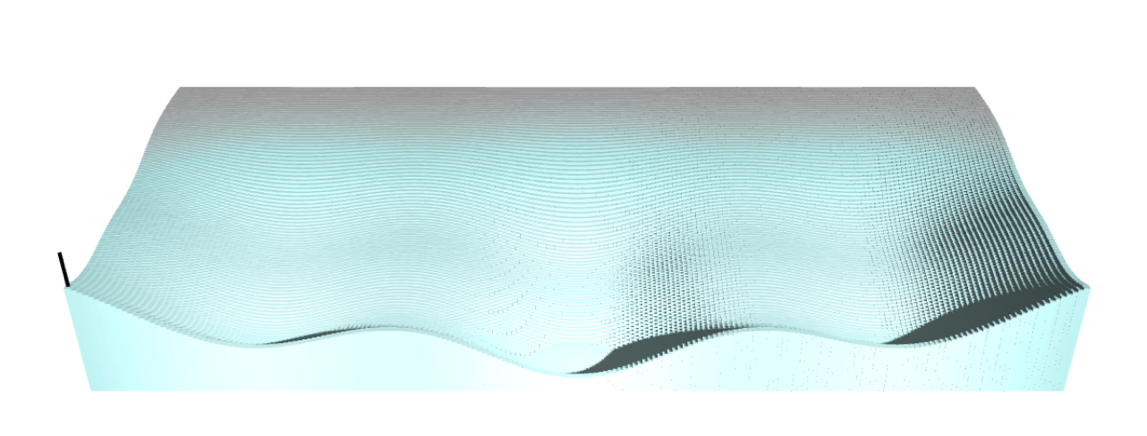
\includegraphics[width=0.4\textwidth]{shuishan.png}}% 子图1的相对位置
	\subfigure[Poplar]{				% 图片2
		\label{fig:yangshu}						% 子图2的标签
		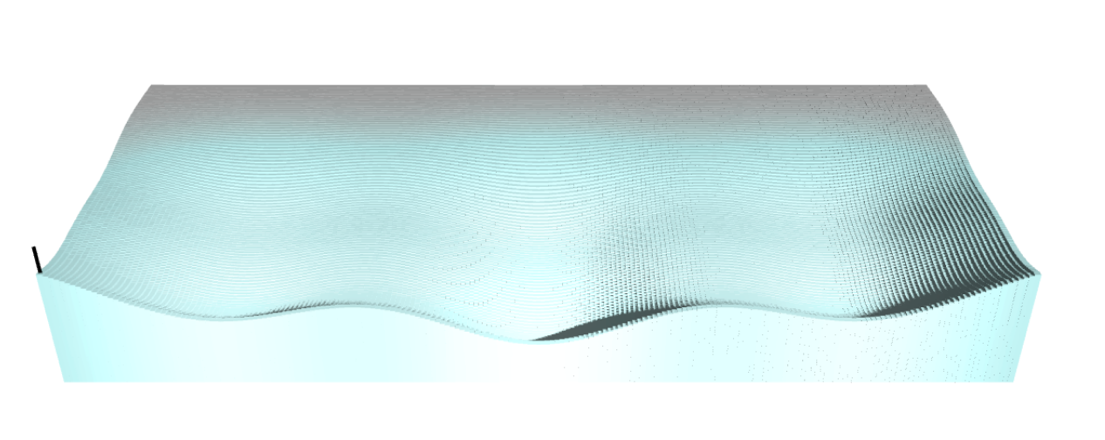
\includegraphics[width=0.4\textwidth]{yangshu.png}}% 子图2的相对位置
    \vspace{-1.0em}
    \\
    \subfigure[Standstone]{				% 图片3([]内为子图标题)
		\label{fig:shayan1}							% 子图3的标签
		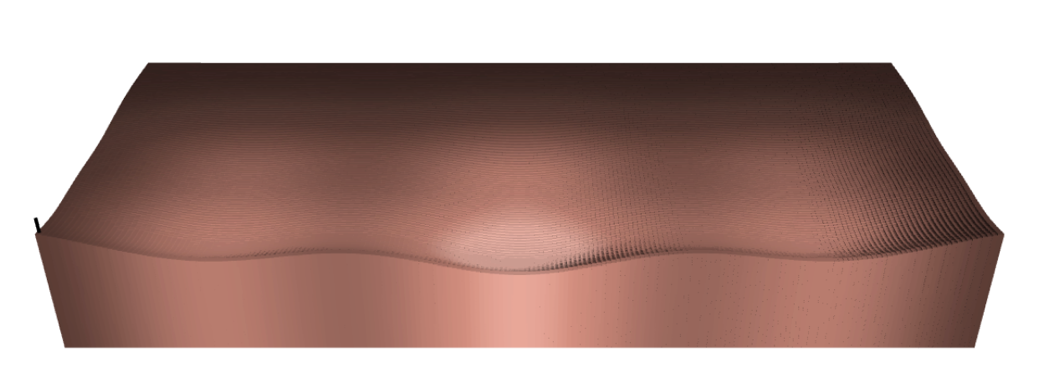
\includegraphics[width=0.4\textwidth]{shayan.png}}% 子图3的相对位置
	\subfigure[Marble]{				% 图片4
		\label{fig:dalishi}						% 子图4的标签
		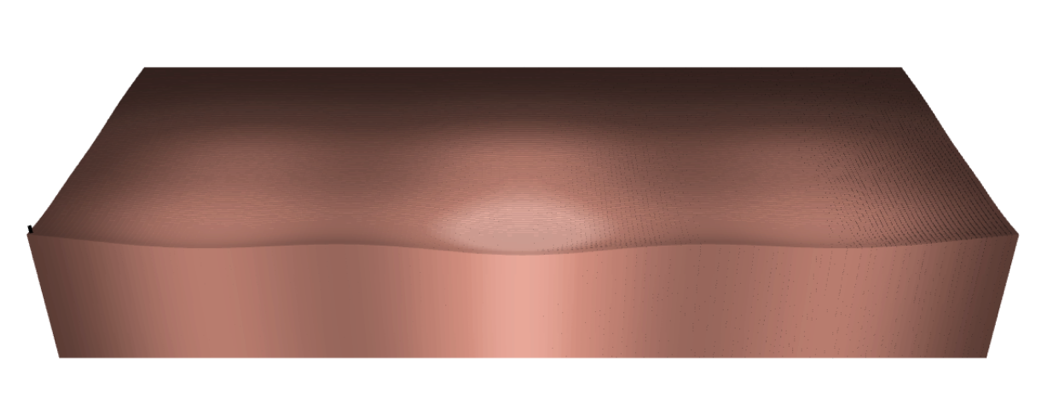
\includegraphics[width=0.4\textwidth]{dalishi.png}}% 子图4的相对位置
	\caption{Simulated wear distribution of wear of different stone and wood}		% 总图标题
	\label{fig:diffh}									% 总图标签
    \vspace{-1.0em}
\end{figure}
As can be seen in \autoref{fig:diffh}, after the same amount of stampede, the incress of $H$ will lead to less wear of the step. Moreover, Figure \autoref{fig:shayan1} exhibits wear patterns similar to those in \autoref{stepwear3}. It provides substantial evidence to support the determination of the source of the step material.





\subsection{People Use The Stair on A Typical Day}
Based on the observation and analysis of human stair usage behavior, we possess some conclusions and gussess. When several individuals use the stairs over an extended period, they tend to walk along the center of the stairs\cite{8}. In such cases, a normal distribution with a small variance is likely to emerge in the X-direction. On the countary, if a large number of individuals use the stairs within a short time, their footsteps become more irregular. It may result in a normal distribution with larger variances or even a multimodal normal distribution. 

To further investigate, we simulated different situations. Divide one day into 1000 time steps For each time step, the probability of one person going upwards is $P_o$  while  the probability of two people going upwards $(1-P_o)$. $P_o$ reflects the number of people walking on the stairs that day. Assume that each of the following points is the main focus of a step. 

We set $P_o$=1,0.8,0.6,0.4,0.2,0 respectively. The visualized simulation results are presented in \autoref{fig:666}, and the corresponding $\sigma$ to  $P_o$ are listed in \autoref{psigma}. 

From the \autoref{fig:666} and Table \ref{psigma}, it can be observed that as $P_o$ increases, $\sigma$ decreases. This indicates that when a few of people use the stairs over a long period, their footsteps are more concentrated in the X direction. Conversely, when lots of people use the stairs in a short time, $\sigma$ increases, and the footsteps are more dispersed. This cooperates well with our expectations.
\begin{figure}[H]
\vspace{-1.0em}
	\centering    
	\subfigure[$P_o$=1]{			% 图片1([]内为子图标题)
		\label{fig:p1}							% 子图1的标签
		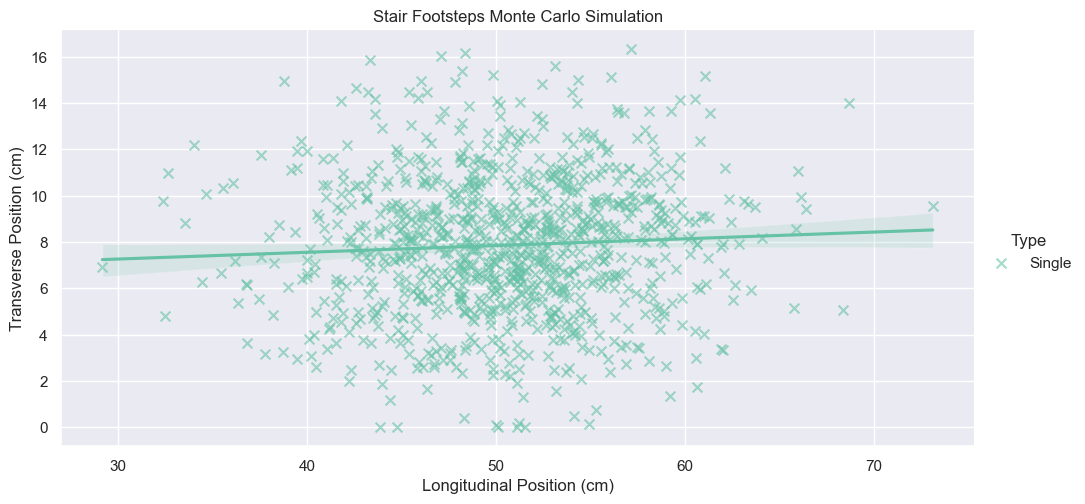
\includegraphics[width=0.5\textwidth]{p1.png}}% 子图1的相对位置
	\subfigure[$P_o$=0.8]{				% 图片2
		\label{fig:p2}						% 子图2的标签
		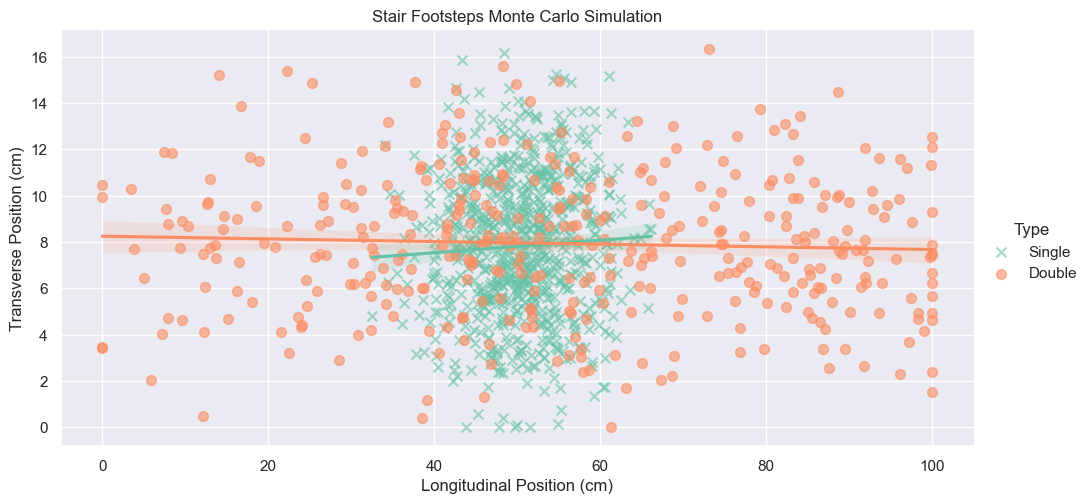
\includegraphics[width=0.5\textwidth]{p08.png}}% 子图2的相对位置
    \vspace{-0.1em}
    \\
    \subfigure[$P_o$=0.6]{				% 图片3([]内为子图标题)
		\label{fig:shayan}							% 子图3的标签
		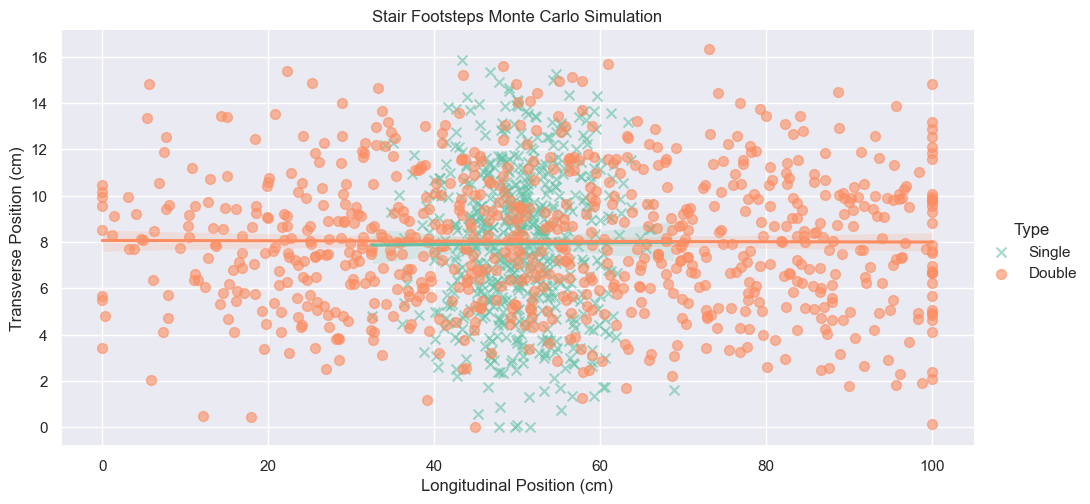
\includegraphics[width=0.5\textwidth]{p06.png}}% 子图3的相对位置
	\subfigure[$P_o$=0.4]{				% 图片4
		\label{fig:dalishi}						% 子图4的标签
		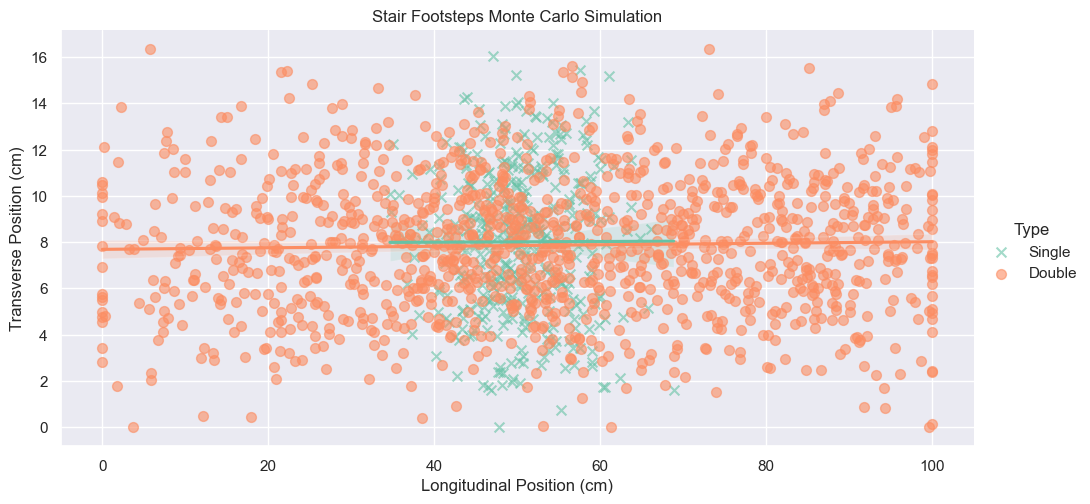
\includegraphics[width=0.5\textwidth]{p04.png}}% 子图4的相对位置
  \vspace{-0.1em}
    \\
    \subfigure[$P_o$=0.2]{				% 图片5([]内为子图标题)
		\label{fig:shayan}							% 子图5的标签
		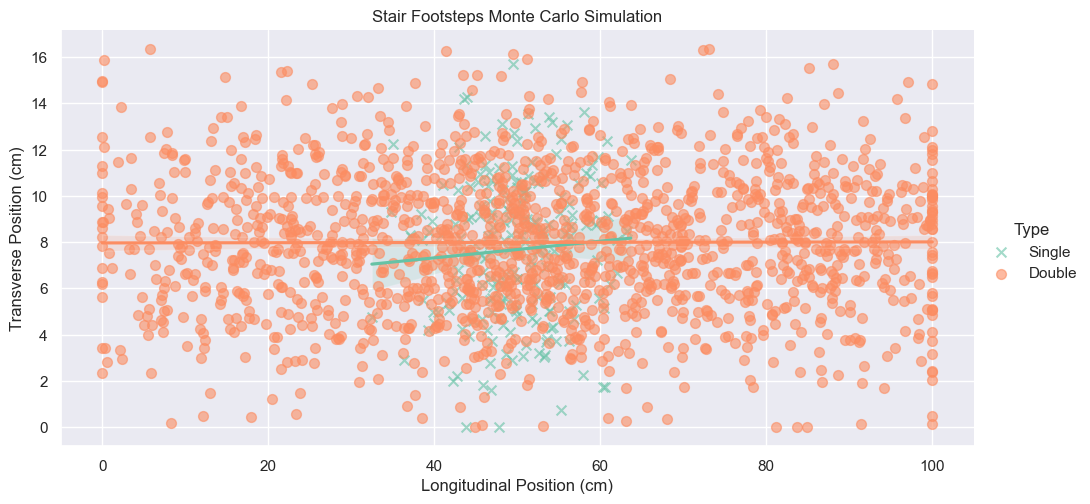
\includegraphics[width=0.5\textwidth]{p02.png}}% 子图5的相对位置
	\subfigure[$P_o$=0]{				% 图片6
		\label{fig:dalishi}						% 子图6的标签
		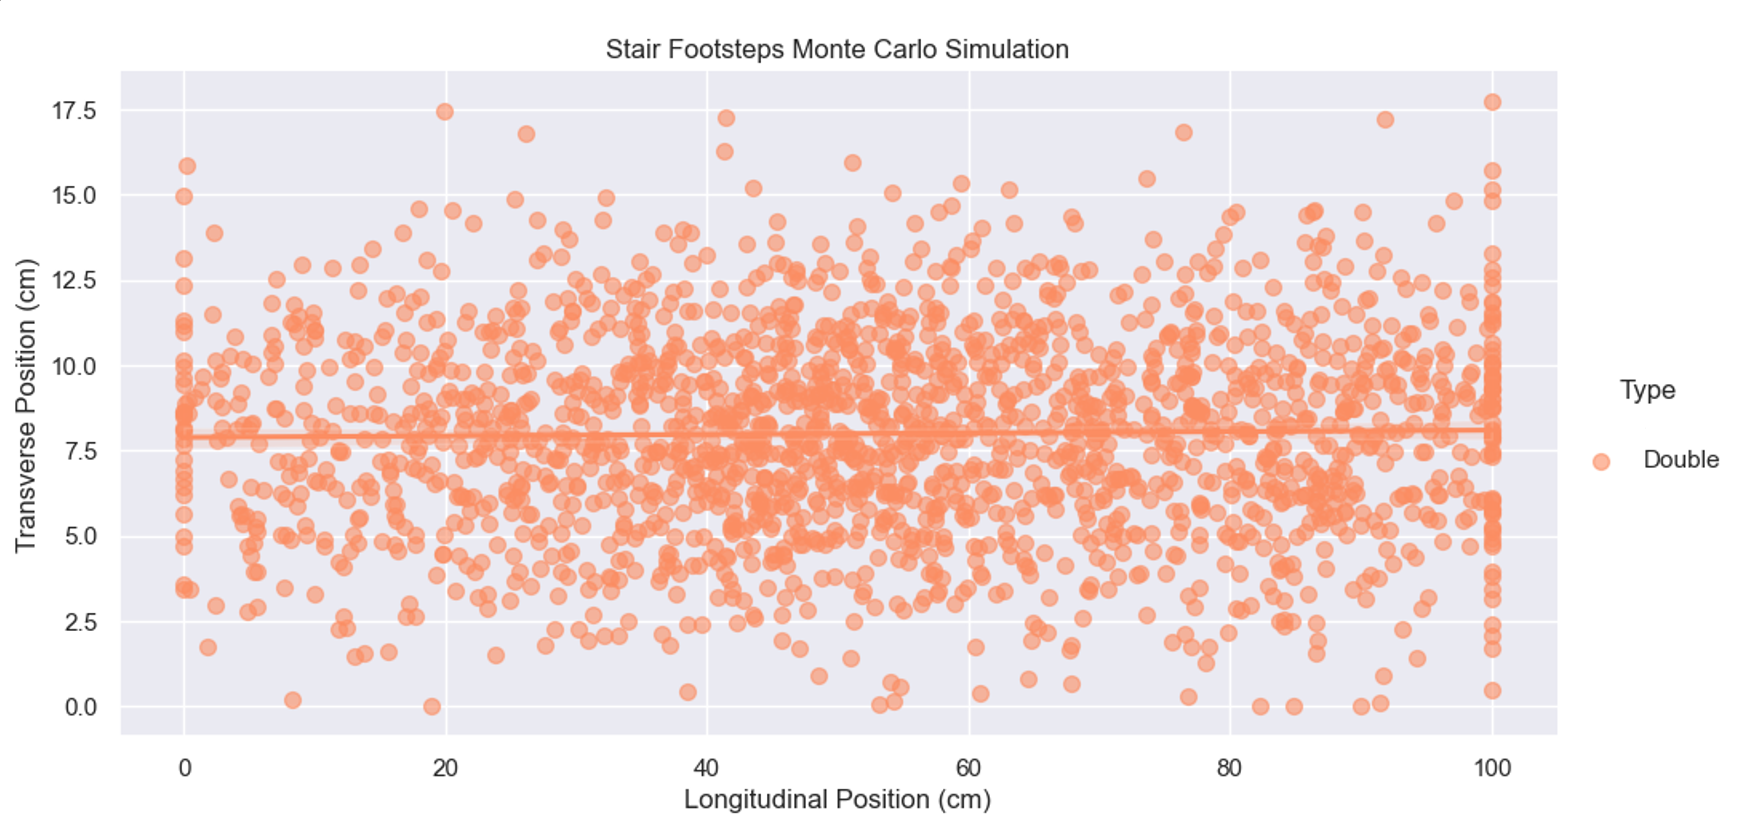
\includegraphics[width=0.5\textwidth]{p00.png}}% 子图6的相对位置
	\caption{Simulated wear conditions of wear of different stone and wood}		% 总图标题
	\label{fig:666}									% 总图标签
    \vspace{-1.0em}
\end{figure}

\begin{table}[H]
    \centering
    \vspace{-0.5em}
    \caption{$\sigma$ for each $p$}
    \vspace{-1.0em}
        \begin{figure}[H]
    	\centering
    	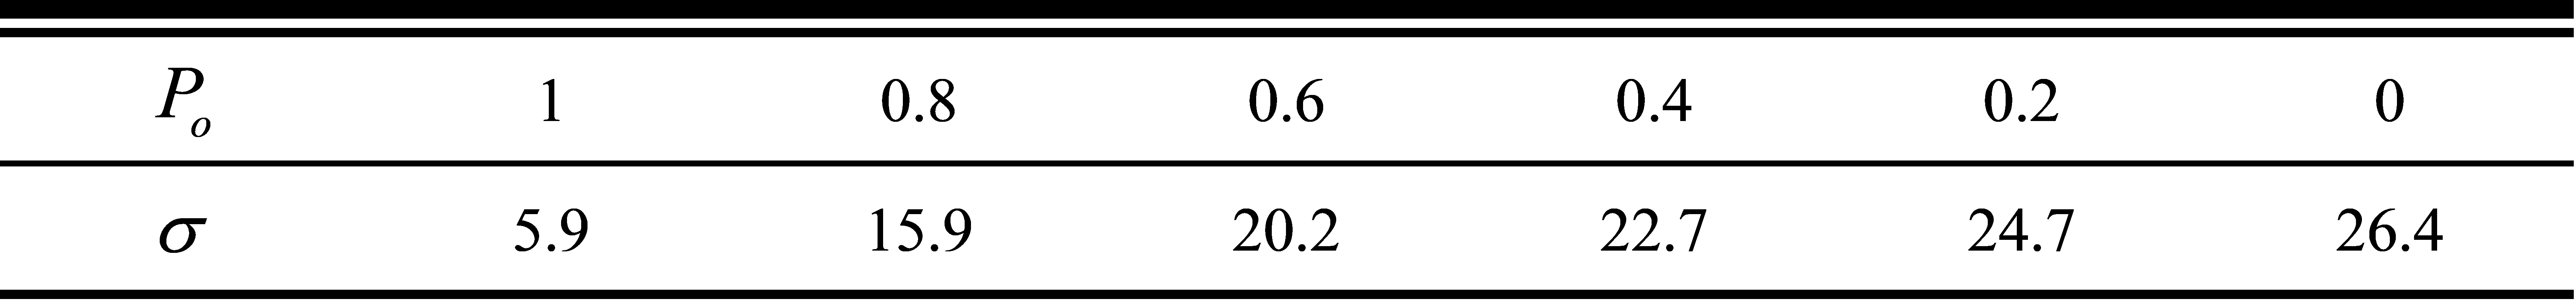
\includegraphics[width=0.8\linewidth]{psigma2.png}
        \end{figure}
    \label{psigma}
    \vspace{-1.5em}
\end{table}
We consider fitting population $Q$ ($Q = (2-P_o)\times 1000$) and the standard deviation $\sigma$. Based on observations, a logarithmic function $y=a\ln{(bx+c)}$ is chosen for least squares fitting. The fitting results are shown in the figure below.

\begin{figure}[H]
\vspace{-1em}
	\centering
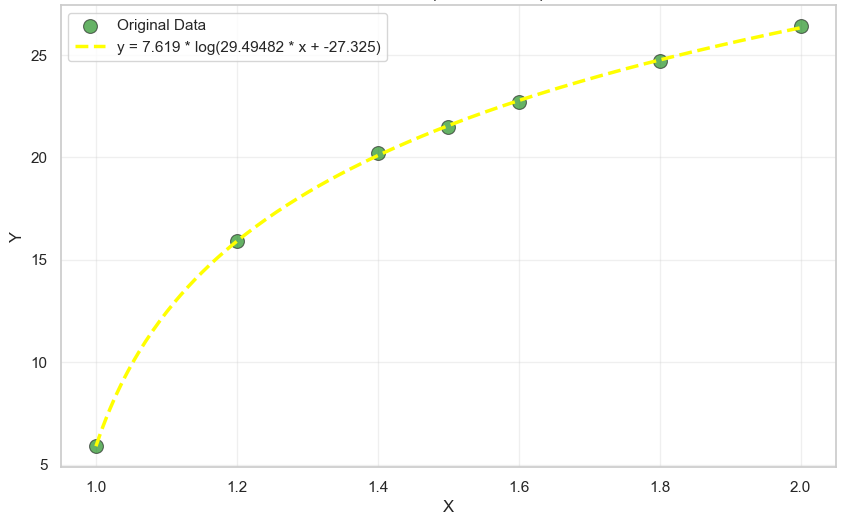
\includegraphics[width=0.5\linewidth]{nihe.png}
	\caption{The fitting curve of $Q$ and $\sigma$}
	\label{nihe}
 \vspace{-1em}
\end{figure}

The coefficient of Determination $R^2$ is 0.9999. From the image and the value of $R^2$, the fit is quite well. Therefore, we obtain the method to estimate the the number of people using stairs frequency of multiple people in a typical day from the edge distribution of the measurement matrix $D_x^{measure}$ . The conclusion can be drawn as:
\begin{equation}
     N_{pass} =0.339e^{0.13125\cdot{\sigma_x}}+0.92338
 \end{equation}
where $\sigma_x$ is the standard deviation in X-direction.

In the measurements of the Edinburgh sandstone steps, the normal variance of the wear depth is 12.1.Therefore, we obtain an average of 1.14 people walking side by side on each step.





\section{Sensitivity and Robustness Analysis}
In our model, we also incorporate parameters closely linked to real-world scenarios. In previous modeling stages, these parameters were determined using data from the ancient stone steps in Edinburgh. However, as scenarios evolve, their value may shift accordingly.
By adjusting these parameters to assess the model’s sensitivity and  robustness, we analyze the results and arrive at the following conclusions.
\subsection{Impact of Material Hardness on Wear Volume}
Under environmental conditions of 30\textcelsius  and 70\% relative humidity ($RH$), the rock wear rate is approximately $p\approx 0.01/$year. The initial hardness $H_0$ values for various materials are as follows: 

Metasequoia: $18 \text{N/mm}^2$, Poplar: $24 \text{N/mm}^2$, Sandstone: $95 \text{N/mm}^2$, Marble: $175 N/mm}^2$\cite{10}.
\begin{figure}[H]

	\centering
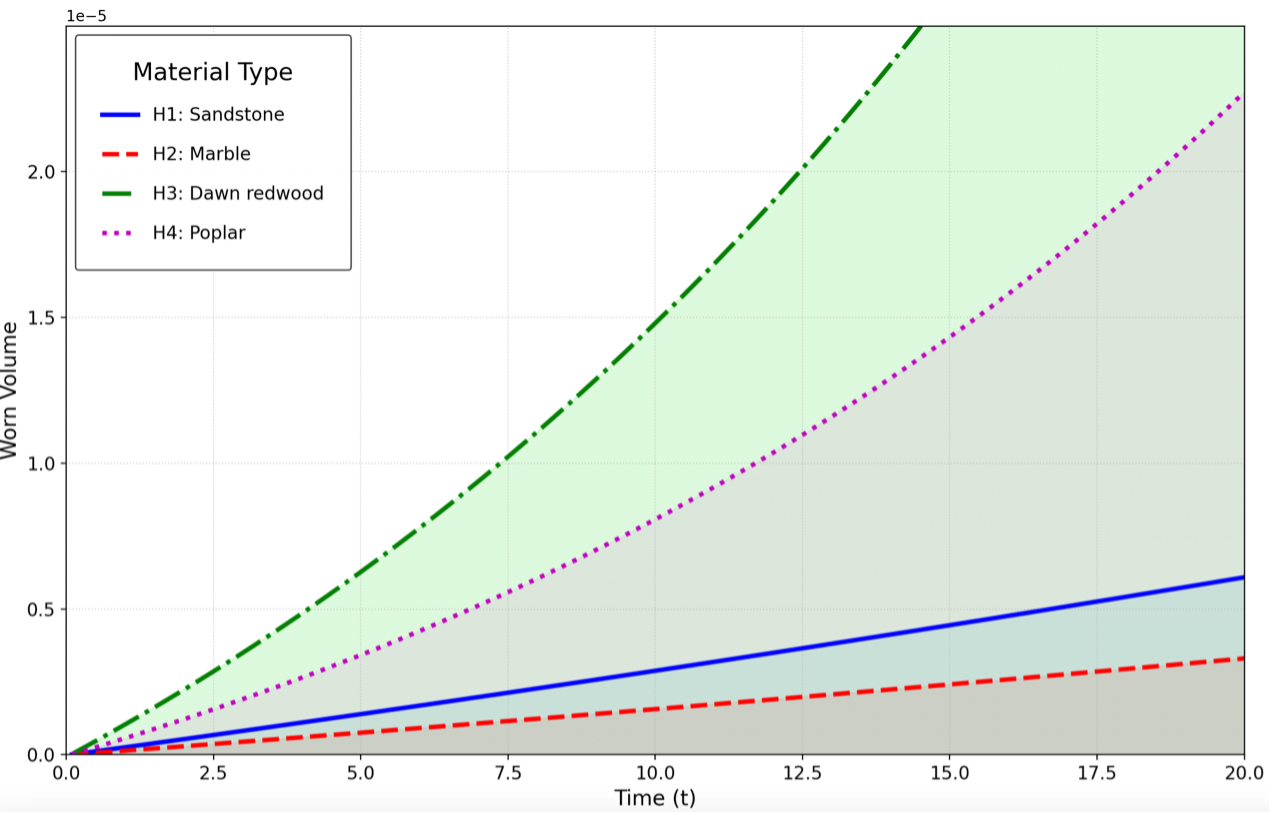
\includegraphics[width=0.5\linewidth]{Hsa.png}
	\caption{Wear accumulation by material hardness $H_0$}
	\label{Hsa}
 \vspace{-1em}
\end{figure}
Based on the analysis results, the initial hardness of wood decreases by 25\%, and after 20 years of wear, it increases by an additional 48.1\%. Meanwhile, the initial hardness of rock decreases by 45.7\%, and after 20 years of wear, it increases by an additional 43.6\%. It can be concluded that our model is sensitive to material hardness. It is feasible to use hardness for relevant calculations.
\subsection{Impact of Weathering Rate Constant on Wear Volume}
Subsequently, we examine how varying the weathering rate constant of rock ($p$) influences the accumulation of wear. Specifically, we set $p$ to 0.0001, 0.0005, 0.0025, and 0.005, then simulate 20 centuries of wear.
\begin{figure}[H]
\vspace{-1em}
	\centering
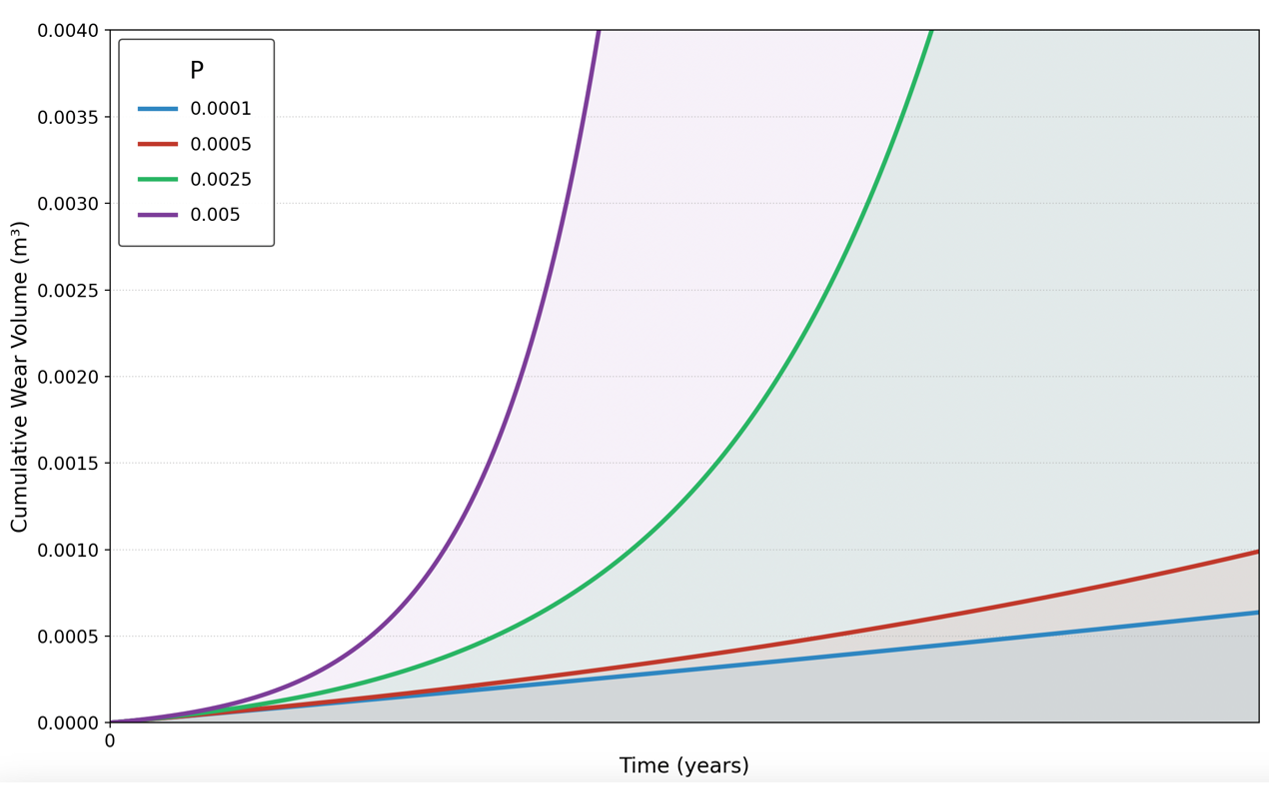
\includegraphics[width=0.5\linewidth]{psa.png}
	\caption{Wear accumulaon by $p$}
	\label{psa}
 \vspace{-1em}
\end{figure}
 When $p$ increases from 0.0025 to 0.005, the time to saturation decreases by 64.2\%.This demonstrates that the wear process is some kind of sensitive to changes in environmental factors or material properties that affect $p$. We can conclude that when the time is relatively short (around 4 centuries), the model is insensitive to $p$. However, when the time is longer, the model becomes highly sensitive to $p$.
\subsection{Impact of Reigon on Wear Volume}
Finally, we test the model's ability to provide more accurate results under varying regional, environmental, and cultural conditions worldwide to test its robustness. We model four countries’ natural and human factors and assume the stone steps are made of granite with an initial hardness $H_0=175\text{N/mm}^2$. 
Using distinct conditions, the model can be tested and refined to account for different climates and usage patterns, thereby enhancing its overall reliability.
\begin{figure}[H]
	\centering
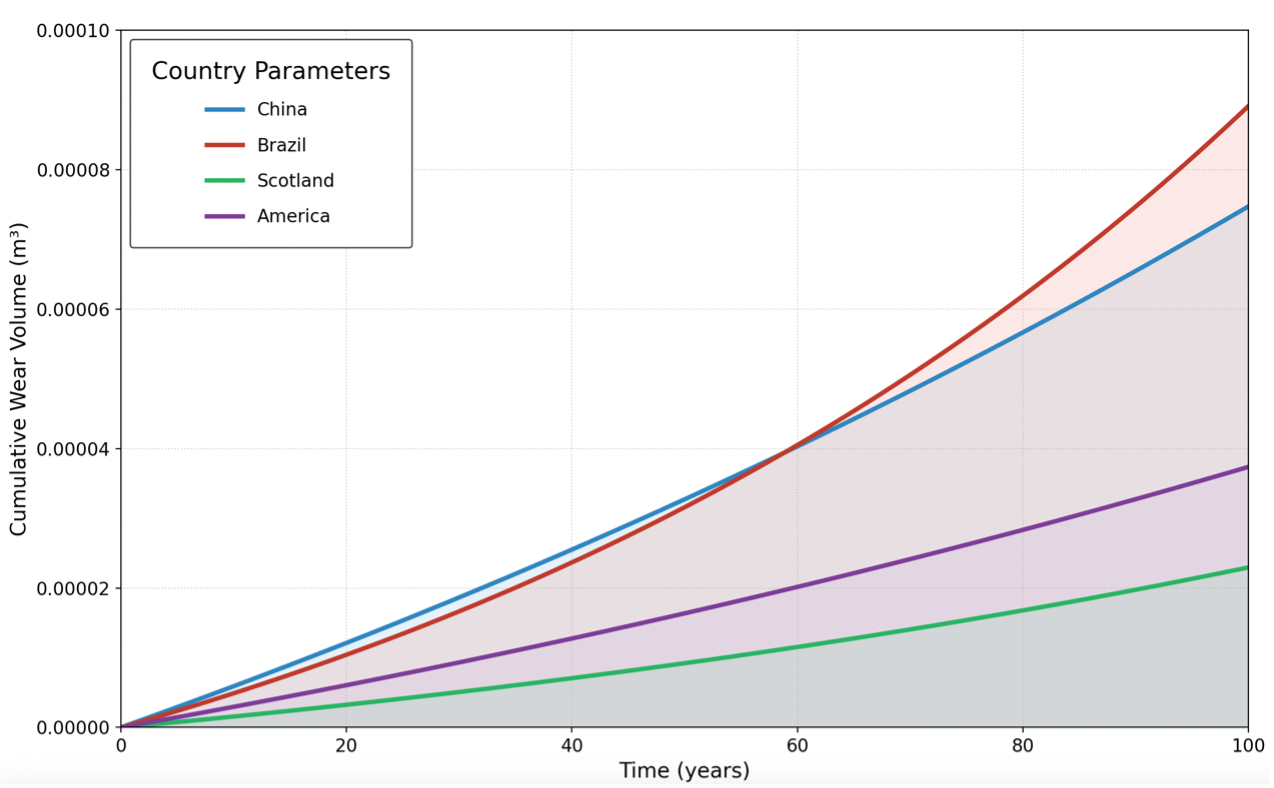
\includegraphics[width=0.5\linewidth]{csa.png}
	\caption{Wear accumulation by country}
	\label{csa}
 \vspace{-1em}
\end{figure}
Over the span of a century, Brazilian stone steps exhibit 0.001\% more wear than Chinese steps, 0.005\% more than American steps, and 0.006\% more than those in Edinburgh.

Because Brazil has high humidity ($RH$ = 80\%), its high corrosion rate ($p$ = 0.012) leads to the fastest wear. Although China and the United States share the same p value, the higher foot traffic in China results in a steeper wear curve. Meanwhile, Scotland’s parameters are moderate, producing an intermediate trend.

However, based on the data, the model demonstrates strong robustness across different regions. Combined with the two previous sensitivity analyses, it can be concluded that our model performs well within a certain timeframe.
\section{Strength and Weakness}
\subsection{Strength}
\begin{enumerate}[\bfseries (1)]
	\setlength{\parsep}{0ex} %段落间距
	\setlength{\topsep}{-1ex} %列表到上下文的垂直距离
	\setlength{\itemsep}{0ex} %条目间距
	\item \textbf{Comprehensive Integration of Factors: }
    The model incorporates mechanical wear, population usage patterns, and material properties, providing a more holistic picture of how wear accumulates.
    \item \textbf{Statistical Treatment of Human Foot Traffic:}
    By using normal (and multi-normal) distributions to capture the variability of footsteps in both the X and Y directions, it reflects realistic pedestrian movement patterns (e.g., single-file vs. parallel use, upward vs. downward traffic).
    \item \textbf{Non-Destructive Measurements:}
    The required data (such as the depth of wear, initial material hardness) can be obtained through non-destructive methods, aligning well with archaeological concerns about preserving heritage.
\end{enumerate}


\subsection{Weakness}
\begin{enumerate}[\bfseries (1)]
	\setlength{\parsep}{0ex} %段落间距
	\setlength{\topsep}{-1ex} %列表到上下文的垂直距离
	\setlength{\itemsep}{0ex} %条目间距
	\item \textbf{Reliance on Simplifying Assumptions:} 
 The model assumes key factors remain fairly consistent over long periods. Real-world usage can fluctuate significantly 
     \item \textbf{Limited Treatment of Environmental Variability:}
     The model uses a single corrosion or wear rate $p$ to represent different humidity or temperature conditions. Realistically, microclimates or seasonal cycles could cause more complex, time-varying wear rates that the model may oversimplify.
\end{enumerate}
\section{Conclusion}
To provide additional assistance to archaeologists, we establisht he Stair Wear Model. This model starts with the wear measure matrix of the research steps and establishes the Wear Volume Model (WVM) and the Wear Distribution Model (WDM). The WVM focuses on the wear volume of the steps and identifies the relationships between the factors causing the wear. The WDM, on the other hand, focuses on the wear distribution, studying how people used these steps in the past. To gather more information and evaluate our model, we identifie consistency and reliability indicators related to wear distribution and age. We also propose some methods to determine the source of the stone step material and  to assess whether repairs had been conducted. Simulations are frequently used in this process. The wear on the steps is inevitable, serving as traces left by people of the past. In the future, we aim to minimize the impact of environmental factors on our stone analysis by introducing more detailed environmental variables. We hope that our model can assist archaeologists in obtaining the information they seek.

\begin{thebibliography}{99}
	\bibitem{1} Li J, Zheng X. Experimental investigation of the stepping dynamics of upstairs walking under time pressure[J]. Physica A: Statistical Mechanics and its Applications, 2023, 622: 128829.
	\bibitem{2} Clark G. Learning Predictive Models for Assisted Human Biomechanics[D]. Arizona State University, 2023.
	\bibitem{3} Cho Y J, Kyung M G, Lee D Y, et al. The difference of in-shoe plantar pressure between level walking and stair walking in healthy males[J]. Gait & Posture, 2022, 97: S93-S94.
	\bibitem{4} Pelit H, Yorulmaz R. Influence of Densification on Mechanical Properties of Thermally Pretreated Spruce and Poplar Wood[J]. BioResources, 2019, 14(4).
	\bibitem{5}Boutrid A, Bensehamdi S, Chaib R. Investigation into Brinell hardness test applied to rocks[J]. World Journal of Engineering, 2013, 10(4): 367-380.
    \bibitem{6}
    World Health Organization (WHO). \textit{Obesity and overweight}. 1 March 2024. [Online]. Available: \url{https://www.who.int/news-room/fact-sheets/detail/obesity-and-overweight}.
	\bibitem{7}Fuhua, W. \textit{Global First Survey Data Results of Obesity Across All Age Groups Released!} \textit{The Lancet}. 2017 Oct 10. [Online]. Available:\url{https://m.medsci.cn/article/show_article.do?id=d98b1161961c}.
     \bibitem{8}Semwal, V.B., Gaud, N., Lalwani, P. et al. Pattern identification of different human joints for different human walking styles using inertial measurement unit (IMU) sensor. Artif Intell Rev 55, 1149–1169 (2022). 
     
    \bibitem{9}Peters, A., Chung, K.  Chu, S. Measurement of gravitational acceleration by dropping atoms. Nature 400, 849–852 (1999). 
    \bibitem{10}\url{https://en.wikipedia.org/wiki/Hardness}
\end{thebibliography}

\end{document}  % 结束$